%==============================================================================
% tento soubor pouzijte jako zaklad
% this file should be used as a base for the thesis
% Autoři / Authors: 2008 Michal Bidlo, 2019 Jaroslav Dytrych
% Kontakt pro dotazy a připomínky: sablona@fit.vutbr.cz
% Contact for questions and comments: sablona@fit.vutbr.cz
%==============================================================================
% kodovani: UTF-8 (zmena prikazem iconv, recode nebo cstocs)
% encoding: UTF-8 (you can change it by command iconv, recode or cstocs)
%------------------------------------------------------------------------------
% zpracování / processing: make, make pdf, make clean
%==============================================================================
% Soubory, které je nutné upravit nebo smazat: / Files which have to be edited or deleted:
%   projekt-20-literatura-bibliography.bib - literatura / bibliography
%   projekt-01-kapitoly-chapters.tex - obsah práce / the thesis content
%   projekt-01-kapitoly-chapters-en.tex - obsah práce v angličtině / the thesis content in English
%   projekt-30-prilohy-appendices.tex - přílohy / appendices
%   projekt-30-prilohy-appendices-en.tex - přílohy v angličtině / appendices in English
%==============================================================================
%\documentclass[]{fitthesis} % bez zadání - pro začátek práce, aby nebyl problém s překladem
%\documentclass[english]{fitthesis} % without assignment - for the work start to avoid compilation problem
\documentclass[zadani]{fitthesis} % odevzdani do wisu a/nebo tisk s barevnými odkazy - odkazy jsou barevné
%\documentclass[english,zadani]{fitthesis} % for submission to the IS FIT and/or print with color links - links are color
%\documentclass[zadani,print]{fitthesis} % pro černobílý tisk - odkazy jsou černé
%\documentclass[english,zadani,print]{fitthesis} % for the black and white print - links are black
%\documentclass[zadani,cprint]{fitthesis} % pro barevný tisk - odkazy jsou černé, znak VUT barevný
%\documentclass[english,zadani,cprint]{fitthesis} % for the print - links are black, logo is color
% * Je-li práce psaná v anglickém jazyce, je zapotřebí u třídy použít 
%   parametr english následovně:
%   If thesis is written in English, it is necessary to use 
%   parameter english as follows:
%      \documentclass[english]{fitthesis}
% * Je-li práce psaná ve slovenském jazyce, je zapotřebí u třídy použít 
%   parametr slovak následovně:
%   If the work is written in the Slovak language, it is necessary 
%   to use parameter slovak as follows:
%      \documentclass[slovak]{fitthesis}
% * Je-li práce psaná v anglickém jazyce se slovenským abstraktem apod., 
%   je zapotřebí u třídy použít parametry english a enslovak následovně:
%   If the work is written in English with the Slovak abstract, etc., 
%   it is necessary to use parameters english and enslovak as follows:
%      \documentclass[english,enslovak]{fitthesis}

% Základní balíčky jsou dole v souboru šablony fitthesis.cls
% Basic packages are at the bottom of template file fitthesis.cls
% zde můžeme vložit vlastní balíčky / you can place own packages here

% Kompilace po částech (rychlejší, ale v náhledu nemusí být vše aktuální)
% Compilation piecewise (faster, but not all parts in preview will be up-to-date)
% \usepackage{subfiles}

% Nastavení cesty k obrázkům
% Setting of a path to the pictures
%\graphicspath{{obrazky-figures/}{./obrazky-figures/}}
%\graphicspath{{obrazky-figures/}{../obrazky-figures/}}

%---rm---------------
\renewcommand{\rmdefault}{lmr}%zavede Latin Modern Roman jako rm / set Latin Modern Roman as rm
%---sf---------------
\renewcommand{\sfdefault}{qhv}%zavede TeX Gyre Heros jako sf
%---tt------------
\renewcommand{\ttdefault}{lmtt}% zavede Latin Modern tt jako tt

% vypne funkci šablony, která automaticky nahrazuje uvozovky,
% aby nebyly prováděny nevhodné náhrady v popisech API apod.
% disables function of the template which replaces quotation marks
% to avoid unnecessary replacements in the API descriptions etc.
\csdoublequotesoff



\usepackage{url}
\usepackage{algorithm}
\usepackage{algpseudocode}

\floatname{algorithm}{Algoritmus}


% =======================================================================
% balíček "hyperref" vytváří klikací odkazy v pdf, pokud tedy použijeme pdflatex
% problém je, že balíček hyperref musí být uveden jako poslední, takže nemůže
% být v šabloně
% "hyperref" package create clickable links in pdf if you are using pdflatex.
% Problem is that this package have to be introduced as the last one so it 
% can not be placed in the template file.
\ifWis
\ifx\pdfoutput\undefined % nejedeme pod pdflatexem / we are not using pdflatex
\else
  \usepackage{color}
  \usepackage[unicode,colorlinks,hyperindex,plainpages=false,pdftex]{hyperref}
  \definecolor{hrcolor-ref}{RGB}{223,52,30}
  \definecolor{hrcolor-cite}{HTML}{2F8F00}
  \definecolor{hrcolor-urls}{HTML}{092EAB}
  \hypersetup{
	linkcolor=hrcolor-ref,
	citecolor=hrcolor-cite,
	filecolor=magenta,
	urlcolor=hrcolor-urls
  }
  \def\pdfBorderAttrs{/Border [0 0 0] }  % bez okrajů kolem odkazů / without margins around links
  \pdfcompresslevel=9
\fi
\else % pro tisk budou odkazy, na které se dá klikat, černé / for the print clickable links will be black
\ifx\pdfoutput\undefined % nejedeme pod pdflatexem / we are not using pdflatex
\else
  \usepackage{color}
  \usepackage[unicode,colorlinks,hyperindex,plainpages=false,pdftex,urlcolor=black,linkcolor=black,citecolor=black]{hyperref}
  \definecolor{links}{rgb}{0,0,0}
  \definecolor{anchors}{rgb}{0,0,0}
  \def\AnchorColor{anchors}
  \def\LinkColor{links}
  \def\pdfBorderAttrs{/Border [0 0 0] } % bez okrajů kolem odkazů / without margins around links
  \pdfcompresslevel=9
\fi
\fi
% Řešení problému, kdy klikací odkazy na obrázky vedou za obrázek
% This solves the problems with links which leads after the picture
\usepackage[all]{hypcap}

% Informace o práci/projektu / Information about the thesis
%---------------------------------------------------------------------------
\projectinfo{
  %Prace / Thesis
  project={DP},            %typ práce BP/SP/DP/DR  / thesis type (SP = term project)
  year={2021},             % rok odevzdání / year of submission
  date=\today,             % datum odevzdání / submission date
  %Nazev prace / thesis title
  title.cs={Simulace skladu a optimalizace rozmístění produktů za účelem zvýšení propustnosti skladu},  % název práce v češtině či slovenštině (dle zadání) / thesis title in czech language (according to assignment)
  title.en={Warehouse Simulation and Product Distribution Optimization for Increased Throughput}, % název práce v angličtině / thesis title in english
  %title.length={14.5cm}, % nastavení délky bloku s titulkem pro úpravu zalomení řádku (lze definovat zde nebo níže) / setting the length of a block with a thesis title for adjusting a line break (can be defined here or below)
  %sectitle.length={14.5cm}, % nastavení délky bloku s druhým titulkem pro úpravu zalomení řádku (lze definovat zde nebo níže) / setting the length of a block with a second thesis title for adjusting a line break (can be defined here or below)
  %Autor / Author
  author.name={Filip},   % jméno autora / author name
  author.surname={Kočica},   % příjmení autora / author surname 
  author.title.p={Bc.}, % titul před jménem (nepovinné) / title before the name (optional)
  %author.title.a={Ph.D.}, % titul za jménem (nepovinné) / title after the name (optional)
  %Ustav / Department
  department={UPGM}, % doplňte příslušnou zkratku dle ústavu na zadání: UPSY/UIFS/UITS/UPGM / fill in appropriate abbreviation of the department according to assignment: UPSY/UIFS/UITS/UPGM
  % Školitel / supervisor
  supervisor.name={Oldřich},   % jméno školitele / supervisor name 
  supervisor.surname={Kodym},   % příjmení školitele / supervisor surname
  supervisor.title.p={Ing.},   %titul před jménem (nepovinné) / title before the name (optional)
  %supervisor.title.a={Ph.D.},    %titul za jménem (nepovinné) / title after the name (optional)
  % Klíčová slova / keywords
  keywords.cs={Sklad, optimalizace, simulace, generátor, objednávka, produkt, pickování, evoluce}, % klíčová slova v českém či slovenském jazyce / keywords in czech or slovak language
  keywords.en={Warehouse, optimization, simulation, generator, order, product, picking, evolution}, % klíčová slova v anglickém jazyce / keywords in english
  %keywords.en={Here, individual keywords separated by commas will be written in English.},
  % Abstrakt / Abstract
  abstract.cs={Tato práce řeší problematiku alokace produktů do lokací ve skladu za pomoci moderních meta-heuristických přístupů v kombinaci s realistickou simulací skladu. Práce poskytuje grafický nástroj umožňující sestavení modelu skladu, generování syntetických zákaznických objednávek, optimalizaci alokace produktů za pomoci kombinace \emph{state of the art} technik, simulátor vytvořeného modelu skladu a nakonec nástroj pro hledání nejkratší cesty objednávky skrze sklad. Práce také uvádí porovnání různých přístupů a experimenty~s~vytvořenými nástroji. Podařilo se optimalizovat propustnost experimentálního skladu na téměř dvojnásobek~--~$\textbf{57\%}$. Přínosem této práce je možnost vytvoření modelu plánovaného či již existujícího skladu a jeho simulace i optimalizace, což může značně zvýšit propustnost skladu a pomoci detekovat a odstranit vytížená místa. To může vést k ušetření zdrojů či pomáhat v plánování. Dále tato práce přináší nový způsob optimalizace skladu a nové optimalizační kritérium.},
  abstract.en={This thesis focuses on the storage location assignment problem using modern meta-heuristic techniques combined with realistic simulation. A graphical tool implemented as part of this work is capable of warehouse model creation, generation of synthetic customer orders, optimization of product allocation using state of the art techniques, extensive warehouse simulation, and a pathfinder capable of finding the shortest path for orders going through the system. The work presents the comparison between different approaches based on many parameters to reach the most efficient allocation of products to warehouse slots. The author conducted tests on an experimental warehouse featuring almost twice the throughput~--~$\textbf{57\%}$. The benefit of this work is a possibility to create model of an already built warehouse and its simulation and optimization, driving impact on the throughput of the warehouse, saving the user's resources, or helping him in planning and bottle-neck identification. Furthermore, this thesis introduces a new approach to warehouse optimization and new optimization criteria.},
  % Prohlášení (u anglicky psané práce anglicky, u slovensky psané práce slovensky) / Declaration (for thesis in english should be in english)
  declaration={Prohlašuji, že jsem tuto diplomovou práci vypracoval samostatně pod vedením pana Ing. Oldřicha Kodyma. Uvedl jsem všechny literární prameny a publikace, ze kterých jsem čerpal.},
  %declaration={I hereby declare that this Bachelor's thesis was prepared as an original work by the author under the supervision of Mr. X
% The supplementary information was provided by Mr. Y
% I have listed all the literary sources, publications and other sources, which were used during the preparation of this thesis.},
  % Poděkování (nepovinné, nejlépe v jazyce práce) / Acknowledgement (optional, ideally in the language of the thesis)
  acknowledgment={Zde bych rád poděkoval svému vedoucímu práce Ing. Oldřichu Kodymovi, konzultantovi Ing. Danielu Chalupovi a Bc. Davidu Vosolovi za cenné rady a podnětné připomínky. Výpočetní zdroje byly poskytnuty projektem \uv{e-Infrastruktura CZ} (e-INFRA LM2018140) v rámci programu \uv{Projects of Large Research, Development and Innovations Infrastructures}.},
  %acknowledgment={Here it is possible to express thanks to the supervisor and to the people which provided professional help
%(external submitter, consultant, etc.).},
  % Rozšířený abstrakt (cca 3 normostrany) - lze definovat zde nebo níže / Extended abstract (approximately 3 standard pages) - can be defined here or below
  %extendedabstract={Do tohoto odstavce bude zapsán rozšířený výtah (abstrakt) práce v českém (slovenském) jazyce.},
  %faculty={FIT}, % FIT/FEKT/FSI/FA/FCH/FP/FAST/FAVU/USI/DEF
  faculty.cs={Fakulta informačních technologií}, % Fakulta v češtině - pro využití této položky výše zvolte fakultu DEF / Faculty in Czech - for use of this entry select DEF above
  faculty.en={Faculty of Information Technology}, % Fakulta v angličtině - pro využití této položky výše zvolte fakultu DEF / Faculty in English - for use of this entry select DEF above
  department.cs={Ústav matematiky}, % Ústav v češtině - pro využití této položky výše zvolte ústav DEF nebo jej zakomentujte / Department in Czech - for use of this entry select DEF above or comment it out
  department.en={Institute of Mathematics} % Ústav v angličtině - pro využití této položky výše zvolte ústav DEF nebo jej zakomentujte / Department in English - for use of this entry select DEF above or comment it out
}

% Rozšířený abstrakt (cca 3 normostrany) - lze definovat zde nebo výše / Extended abstract (approximately 3 standard pages) - can be defined here or above
%\extendedabstract{Do tohoto odstavce bude zapsán výtah (abstrakt) práce v českém (slovenském) jazyce.}

% nastavení délky bloku s titulkem pro úpravu zalomení řádku - lze definovat zde nebo výše / setting the length of a block with a thesis title for adjusting a line break - can be defined here or above
%\titlelength{14.5cm}
% nastavení délky bloku s druhým titulkem pro úpravu zalomení řádku - lze definovat zde nebo výše / setting the length of a block with a second thesis title for adjusting a line break - can be defined here or above
%\sectitlelength{14.5cm}

% řeší první/poslední řádek odstavce na předchozí/následující stránce
% solves first/last row of the paragraph on the previous/next page
\clubpenalty=10000
\widowpenalty=10000

% checklist
\newlist{checklist}{itemize}{1}
\setlist[checklist]{label=$\square$}

\begin{document}
  % Vysazeni titulnich stran / Typesetting of the title pages
  % ----------------------------------------------
  \maketitle
  % Obsah
  % ----------------------------------------------
  \setlength{\parskip}{0pt}

  {\hypersetup{hidelinks}\tableofcontents}
  
  % Seznam obrazku a tabulek (pokud prace obsahuje velke mnozstvi obrazku, tak se to hodi)
  % List of figures and list of tables (if the thesis contains a lot of pictures, it is good)
  \ifczech
    \renewcommand\listfigurename{Seznam obrázků}
  \fi
  \ifslovak
    \renewcommand\listfigurename{Zoznam obrázkov}
  \fi
  % {\hypersetup{hidelinks}\listoffigures}
  
  \ifczech
    \renewcommand\listtablename{Seznam tabulek}
  \fi
  \ifslovak
    \renewcommand\listtablename{Zoznam tabuliek}
  \fi
  % {\hypersetup{hidelinks}\listoftables}

  \ifODSAZ
    \setlength{\parskip}{0.5\bigskipamount}
  \else
    \setlength{\parskip}{0pt}
  \fi

  % vynechani stranky v oboustrannem rezimu
  % Skip the page in the two-sided mode
  \iftwoside
    \cleardoublepage
  \fi

  % Text prace / Thesis text
  % ----------------------------------------------
  \ifenglish
    \input{projekt-01-kapitoly-chapters-en}
  \else
    \chapter{Úvod}
% Motivace
Sklady jsou klíčová část dodavatelského řetězce, kam jsou dočasně uloženy produkty z~výroby, než jsou odeslány k~zákazníkům~v~rámci objednávek. Simulace, automatizace a optimalizace skladů se vzhledem k rostoucím nárokům na jejich výkonnost a propustnost v~posledních letech značně rozšířila. Automatizace a optimalizace skladu, ač velmi nákladný proces, může společnosti přinést nebývalé zvýšení produktivity, bezpečnosti a v neposlední řadě také kvality, respektive menší chybovosti.

% Problém
Sklady se zpravidla optimalizují za účelem rychlejšího odbavování zákaznických objednávek. Každá objednávka sestává z několika položek, kde každá položka jednoznačně identifikuje zakoupený produkt a jeho požadované množství. Objednávky jsou typicky vyřizovány ve formě kartonu, do kterého se vloží zakoupené produkty (popřípadě faktura, atp.) a karton se odešle k zákazníkovi. Vyřizování objednávek v rámci skladu poté sestává z cestování kartonu mezi lokacemi po dopravnících a vybírání požadovaných produktů ze slotů lokací (úložné prostory, kde jsou produkty dočasně uloženy) do kartonů objednávek. Proces sbírání zakoupených produktů do kartonů je obecně označován jako pickování objednávek. Plynulost a efektivita pickování objednávek, které jsou ovlivněny mimo jiné rozložením produktů, mají zásadní vliv na výkonnost skladu jako celku, a proto jsou často považovány za nejslibnější oblast z hlediska optimalizace skladových operací~\cite{optimisationOrderPickingGA}. Tato práce řeší primárně kombinatorický NP-těžký problém, a sice jakým způsobem rozmístit produkty do slotů lokací ve skladu, aby bylo dosaženo co nejvyšší propustnosti. Tato problematika se v literatuře označuje jako SLAP (\emph{storage location assignment problem}).

% Existující práce
Z množství vědeckých příspěvků, které se v posledních letech zabývaly problematikou SLAP lze usuzovat, že je to velmi aktivní a diskutované téma. Z obsahu těchto příspěvků pak lze usuzovat, že toto téma není zdaleka vyřešené, a existuje zde velký potenciál pro možná zlepšení, a to zejména z pohledu zvýšení výkonnosti skladů.

% Způsob řešení
V navrženém řešení uživatel nejprve provede vytvoření modelu skladu v grafickém 2D editoru dle jeho potřeb. Poté si vygeneruje data pomocí \textbf{generátoru objednávek}, který na základě pravděpodobnostních modelů generuje sady zákaznických objednávek pro trénování a testování. Na základě modelu skladu a vygenerovaných objednávek může následně uživatel provést realistickou \textbf{simulaci skladu}, nebo pomocí nástroje \textbf{hledač cest} (dále jako pathfinder) nalézt optimální cestu objednávky skladem pomocí mravenčího algoritmu. Dále je uživatel schopen provést \textbf{optimalizaci rozložení produktů} ve skladu za účelem zvýšení propustnosti skladu pomocí čtyř evolučních algoritmů. Veškeré zmíněné funkcionality reprezentované jednotlivými nástroji jsou jednak použitelné samostatně skrze příkazovou řádku, ale také spojeny do jednoho grafického nástroje, nazvaného \textbf{skladový manažer} (dále jako Warehouse Manager). Hlavním přínosem tedy bude zvýšení propustnosti skladu, a to díky hned několika optimalizačním technikám, které jsou v dokumentu porovnány.

% Zhodnocení (prodání)
Vytvořené řešení je zcela nezávislé na modelu skladu, ten si lze vytvořit zcela libovolně, narozdíl od velké části existujících řešení. Výsledky optimalizace jsou u menších až středních skladů na velmi vysoké úrovni, ačkoli se zvyšující se komplexitou skladu se kvalita optimalizace lehce snižuje. Mimo optimalizaci rozložení produktů ve skladu poskytuje řešení další užitečné funkcionality, jako je například identifikace úzkých míst (tzv. \emph{bottlenecků}) či nalezení nejkratší cesty objednávky skrze sklad.

% Struktura dokumentu
Kapitola \ref{SLAP} se zabývá obecným popisem problematiky alokace produktů do lokací a~souhrnem existujících přístupů. V kapitole \ref{EA} lze nalézt popis evolučních algoritmů a jejich redefinici pro diskrétní prostor. Kapitoly \ref{navrhNastroju} a~\ref{implementaceNastroju} popisují návrh a implementaci pěti nástrojů vytvořených v rámci této práce. Kapitola \ref{vyhodnoceniNastroju} poté shrnuje dosažené výsledky práce.



\chapter{Problematika rozmístění produktů do lokací ve skladu}
\label{SLAP}
Tato kapitola pojednává o problematice rozmístění produktů do lokací, anglicky zvané \emph{Storage Location Assignment Problem}, dále pouze zkratka SLAP. V odborné literatuře se lze však setkat s různými variacemi označeními této problematiky, avšak se stejným významem (např.: \emph{Storage Assignment}, \emph{Product allocation/location}, \emph{Slotting}, a~tak dále). Při studiu této problematiky jsem vycházel~z~\cite{slapSeacomp, optimisationOrderPickingGA, exactTimeSlap, whModelSim, slapReview, slapGaMultiObj, slapPickAndPass}.


%%%%%%%%%%%%%%%%%%%%%%%%%%%%%%%%%%%%%%%%%%%%%%%%%%%%%%%%%%%%%%%%%%%%%%%%%%%%%%%%%%%%%%%%%%%


\section{Motivace pro efektivní optimalizaci skladu} % nebo Motivace pro řešení SLAP
\label{motivace}
Sklady slouží pro dočasné uložení produktů (typicky z produkce), které jsou následně postupně získávány za účelem vyřízení zákaznických objednávek. \uv{Pickování} zákaznických objednávek je proces při kterém jsou takto uložené produkty systematicky hledány a přemisťovány z úložných prostor (přesněji slotů lokací), ve kterých jsou dočasně uloženy, do kartonů, ve kterých jsou následně odeslány k zákazníkům. Zákaznické objednávky typicky sestávají z jednotlivých položek, anglicky zvaných \emph{order line}, vždy představující jeden produkt (v anglické literatuře často označován jako \emph{article}, \emph{product}, \emph{code} či \emph{stock keeping unit}) a jeho požadovanou kvantitu (množství). Způsob organizace produktů a jejich pickování značně ovlivňuje výkonnost celého skladu a tedy ovlivňuje efektivnost celého dodavatelského řetězce. To znamená, že čím rychleji budou produkty napickovány, tím rychleji se zákaznická objednávka vyřídí~\cite{optimisationOrderPickingGA}.

Pickování objednávek je jedna z časově nejnáročnějších operací prováděných ve skladu a~je spojena s $55\%$ celkových nákladů skladu, a proto se tedy dle vědců jeví jako nejvhodnější oblast pro optimalizace skladu~\cite{optimisationOrderPickingGA}.

\addtocounter{footnote}{-1}

\begin{figure}[t]
    \centering
    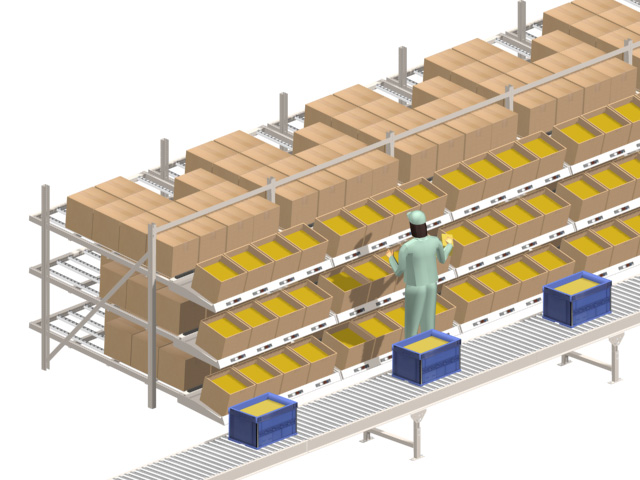
\includegraphics[width=0.8\linewidth]{figures/slap_ea/location_rack.jpg}
    \caption{Příklad pickování objednávek pro vysvětlení terminologie\protect\footnotemark{}. Na obrázku lze vidět lokaci a pickera (pracovník skladu, který vytahuje produkty ze slotů lokace do kartonů objednávek). Způsob fungování je následující: po dopravníku přijede karton, který reprezentuje nějakou objednávku. Uživatel tento karton naskenuje. Systém následně zjistí, které produkty tato objednávka potřebuje, a ukazuje uživateli které produkty (z jakých slotů) má do tohoto kartonu vkládat. Po každém vložení produktu do kartonu uživatel tuto akci potvrdí a pokračuje dalším produktem. Až nasbírá všechny produkty, které jsou na této lokaci potřeba napickovat, systém uživateli řekne, ať karton vloží na dopravník (odkud pokračuje dál), a aby naskenoval další karton, u kterého bude postupovat podobným způsobem.}
    \label{fig:locationRackExplained}
\end{figure}

Proces průmyslové automatizace způsobil požadavky na automatizované skladové systémy v mnoha různých odvětvích. Typické činnosti v takovýchto skladech jsou: příjem zákaznických objednávek a jejich seskupování, třídění a plánování v závislosti na aktuálním množství jednotlivých produktů ve skladu, postupné spouštění objednávek a jejich pickování, až po proces odesílání ze skladu k zákazníkům. Proces pickování objednávek sestává z~několika částí, které značně závisí na typu skladu, jeho komplexitě a v neposlední řadě na použitém informačním systému. Příklad takového pickování společně s popisem terminologie lze vidět na snímku \ref{fig:locationRackExplained}~\cite{whModelSim, optimisationOrderPickingGA}. 

Z pohledu složitosti se SLAP klasifikuje jako NP-těžký problém, a to vzhledem k množství variací způsobených množstvím produktů a úložných prostor. Vzhledem k tomu, mnoho meta-heuristických a heuristických metod bylo použito za účelem řešení této problematiky. Pokud je počet produktů roven počtu úložných prostor, jedná se o problém QAP\footnotemark{}. Pokud počet produktů převyšuje počet úložných prostor, jedná se o problém Knappsack~\cite{slapReview}.

Strategie uložení produktů hraje důležitou roli z pohledu skladových informačních systémů (ang. \emph{warehouse management system}). Tato operace je mnohdy mylně považována za snadnou, ale ve skutečnosti kvůli nejistotě požadavků, variabilitě druhů produktů a potřebě okamžité reakce na změnu na trhu je velmi komplexní a vyžaduje složitá rozhodnutí. Je nutné, aby sklady byly navrženy a řízeny tak, aby byly nákladově efektivní. Náklady na fungování skladu jsou do značné míry určovány již ve fázi návrhu a proto je vhodné před samotnou stavbou skladu věnovat značnou pozornost studiu a analýze budoucího skladu pro dosažení co nejoptimálnějšího skladu pro daný \emph{use-case} (česky případ užití)~\cite{slapSeacomp, slapReview}.

\addtocounter{footnote}{-1}

\footnotetext{Obrázek převzat z \url{http://orderpickingfastfetch.blogspot.com/2013/01/what-is-pick-to-light-pick-to-light-or.html}.}

\stepcounter{footnote}
\footnotetext{QAP -- \emph{Quadratic assignment problem} -- česky problematika kvadratického rozřazení.}

Problematika rozmístění produktů do úložných lokací ve skladu se snaží o nalezení co nejefektivnějšího rozřazení jednotlivých produktů do lokací ve skladu za účelem snížení doby potřebné k vyřízení zákaznických objednávek. To následně velmi ovlivňuje KPI\footnote{KPI -- \emph{Key performance indicators} -- česky výkonnostní klíčové indikátory}~\cite{slapPickAndPass}.

\section{Strategie uložení produktů}
Vzhledem k variabilitě parametrů produktů, které mohou být ve skladu ukládány, existují různé strategie (někdy také zvané jako politiky) uložení produktů do úložných prostor skladu. Při použití skladového informačního systému se tyto možnosti ještě rozšiřují, protože informační systém umožňuje značně větší kontrolu nad celým skladem. Základní strategie pro ukládání produktů jsou následující~\cite{slapSeacomp}\cite{slapPickAndPass}:

\begin{itemize}
    \item \emph{\textbf{Fixed slot}} politika -- Každý slot každé lokace skladu má pevně přiřazený produkt, který obsahuje. Toto nastavení je neměnné. Pro tuto politiku není třeba žádný informační systém a je nejvhodnější z pohledu optimalizací (použito v této práci).
    \item \emph{\textbf{Random}} politika -- Jak z jména vyplývá, produkty jsou rozřazeny do slotů náhodně, což z této politiky dělá jednu z nejlehčích metod. Je velmi rozšířená, protože často vyžaduje méně místa než ostatní metody a umožňuje efektivnější využití úložných prostor. Je také často použita pro srovnání při vyhodnocování výkonnosti ostatních politik.
    \item \emph{\textbf{Frequency-based} politika} -- Přiřazuje nejčastěji pickované/kupované produktu do slotů, které jsou nejblíže ke vstupu a výstupu ze skladu, za účelem sínížení celkové doby zpracování objednávek (použito v této práci pro porovnání).
    \item \emph{\textbf{Class-based} politika} -- Je kompromis mezi jednoduchostí náhodné politiky a přesností (komplexností) politiky založené na frekvenci pickování.
\end{itemize}

Toto je výčet pouze základních politik pro ukládání produktů. Tyto politiky lze mezi sebou dále kombinovat a vytvářet tak složitější, ale účinnější politiky.


\section{Nástroje pro optimalizaci skladu}
Při studiu této podkapitoly jsem vycházel z práce \cite{slapSeacomp}. Nástroj pro optimalizaci skladu by měl být schopen plnit tyto úlohy:

\begin{itemize}
    \item Vytvoření modelu skladu -- Tj. pozice vstupů, výstupů, jednotlivých lokací (včetně množství obsažených slotů), apod. Způsob, jakým jsou jednotlivé zařízení ve skladu rozmístěny se označuje jako layout skladu.
    \item Datovou analýzu -- Na základě (typicky historických) dat -- např. objednávek zákazníků -- poskytovat agregované či na pouhý pohled neviditelné informace, typicky využité jako podpora při rozhodování.
    \item Podporu při rozhodování -- Pomoct uživatelům nástroje při rozhodnutích, jako například jak efektivně rozmístit jednotlivé prvky skladu či produkty do lokací.
    \item Kontrola a řízení zboží na skladě -- sem spadá mj. také doplňování produktů (ang. \emph{replenishment}).
\end{itemize}

Snadno upravitelný layout skladu pak může uživateli pomoct při takzvaných \emph{what-if} (v~překladu co-kdyby) a \emph{as-is} (jak-je) analýzách~\cite{slapSeacomp}:

\begin{itemize}
    \item Analýza \emph{what-if} -- Může být provedena na základě virtuálního přerovnání layoutu skladu pomocí konfiguračního nástroje a opětovného vyhodnocení a porovnání KPI.
    \item Analýza \emph{as-is} -- Může být provedena na základě \textbf{již existujícího} layoutu skladu za účelem vyhodnocení KPI.
\end{itemize}

\begin{figure}[t]
    \centering
    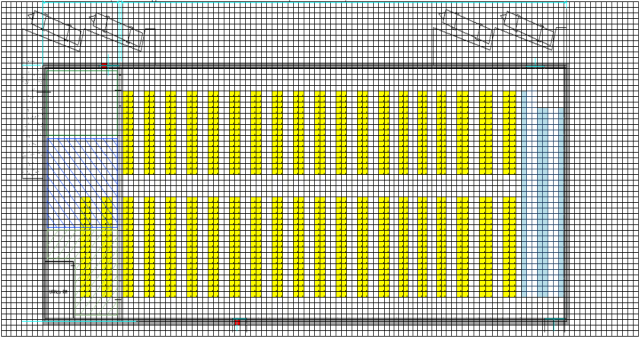
\includegraphics[width=0.99\linewidth]{figures/slap_ea/DesignTool.png}
    \caption{Na obrázku je možné vidět příklad jednoduchého nástroje pro tvorbu modelu skladu, a také v něm vytvořeného modelu skladu. Obrázek převzat z práce~\cite{slapSeacomp}.}
    \label{fig:slapDesignTool}
\end{figure}

Příklad toho, jak může vypadat takový nástroj pro vytvoření virtuálního modelu skladu lze vidět na obrázku~\ref{fig:slapDesignTool}. V závislosti na možnostech nástroje je uživatel schopen si sám jednoduše vytvořit virtuální reprezentaci svého existujícího skladu (měřítko vůči reálnému světu, pozice lokací a slotů, vstupů a výstupů skladu, či dopravníků propojující jednotlivé komponenty). Tato reprezentace může uživateli pomoct při rozhodování za pomoci zmíněných analýz.

\section{Simulace skladu}
Automatizované sklady jsou velmi komplexní systémy. Často mají mnohá omezení daná jejich layoutem, způsobem manipulace s produkty (dopravníky, vysokozdvižné vozíky, \ldots), úložnými a pickovacími politikami, a tak dále. Optimalizace výkonnosti takovýchto skladů často vyžaduje přesnou definici jejich modelu. Zmíněné praktiky jako ukládání či pickování produktů nelze jednoduše převést na matematické výrazy, které by šly optimalizovat standardním způsobem. Optimalizace takovýchto systémů je navíc často více-objektivní (např. co nejkratší doba pickovaní a zároveň co nejvyšší úspora místa), kdy se optimalizuje více parametrů zároveň a hledá se množina možných řešení která představuje kompromisy (ang. \emph{tradeoff}) mezi různými požadavky. Z toho vyplývá, že lepší způsob jak se vypořádat s řešením tohoto problému je pomocí programovacích technik, což de-facto znamená vytvořit simulátor skladu, odpovídající pokud možno co nejvíce reálnému modelovanému systému~\cite{whModelSim}.

Skladové systémy jsou vzhledem k jejich důležitosti v dodavatelském řetězci a potřebě optimalizace (resp. velké úspoře prostředků při jejich optimalizaci) velmi často předmětem simulování. V nejedné práci zabývající se problematikou SLAP se objevují nástroje pro simulaci skladu (příjem, pickování a odesílání objednávek, atp.). Tyto nástroje jsou nejčastěji založeny na diskrétních událostech. V posledních letech se však také objevují řešení založená na agentech. Simulace bývá zpravidla využívána za účelem sledování změn chování při použití různých strategií či konfigurací. Simulátor skladu byl využit například za účelem porovnání ujetých vzdáleností při použití různých strategií uložení produktů v automatizovaném prostředí skladu či vlivu použité alokace slotů na proces manuálního pickování objednávek~\cite{slapReview}.

Práce~\cite{whModelSim} definuje důležitost simulace skladu následujícími úkoly, jež dokáže plnit:

\begin{itemize}
    \item Poskytnutí tzv. \emph{proof-of-concept} (návrh konceptu).
    \item Analýza dopadů na potencionální změny v existujícím systému.
    \item Evaluace výkonnosti skladu již ve fázi návrhu, a to při různém zatížení.
    \item Optimalizace parametrů skladu (layout, úložné a pickovací politiky, \ldots).
    \item Analýza možných \uv{úzkých bodů} (ang. \emph{bottleneck}).
    \item Odhad neměřitelných proměnných a kvantit.
    \item Průzkum a testování nových skladových politik.
    \item Plánování kapacit skladu.
    \item Zodpovězení \emph{what-if} otázek (analýza).
\end{itemize}

Přístupy k simulaci skladu jsou tři. Buď lze využít existujících grafických aplikací, frameworků/knihoven či specializovaných programovacích jazyků. Grafické aplikace sice nevyžadují nutnost psaní kódu a vytvoření systémů je poměrně jednoduché, avšak jsou zpravidla velmi komplexní, drahé a nemusí poskytovat všechny potřebné funkcionality. Patří sem např. AutoMod\textsuperscript{TM} nebo Siemens Tecnomatix\textsuperscript{TM}. Softwarové knihovny poskytují programátorům před-připravené třídy a funkce, které jim pomohou k vytvoření vlastního simulátoru a jsou zpravidla založeny na simulaci diskrétními událostmi. Nevýhodou těchto knihoven je, že většina z nich je orientovaná na simulaci počítačových sítí a ve většině případů je nelze použít pro simulaci skladu (např. OMNeT++ a Ns2). V poslední řadě se používají specializované programovací jazyky mezi které patří např. SIMSCRIPT a SIMULA. Tyto jazyky ulehčují modelování problému pomocí sady před-připravených konstrukcí a instrukcí a jsou často zakomponovány v grafických aplikacích zmíněných výše. Mají však jistá omezení podobně jako softwarové knihovny~\cite{whModelSim}.

V této práci je využit druhý přístup a sice softwarová knihovna, která je zdarma k~použití, kompatibilní se zbytkem C++ programu a flexibilní.


\section{Související práce}
Současná odborná literatura zabývající se problematiku SLAP lze rozdělit do různých kategorií. Nejdůležitější jsou však dvě, a sice použitý přístup a optimalizovaná kritéria, viz~\ref{fig:grafPristupy}~a~\ref{fig:grafMeritka}. Tato práce kombinuje meta-heuristiku se simulací a optimalizovaným kritériem je čas zpracování sady objednávek. V tabulce \ref{tab:klasifikacePraci} lze vidět veškeré studované práce zabývající se problematikou SLAP klasifikované dle těchto kritérií~\cite{slapReview}.

\begin{table}[t]
\centering
\begin{tabular}{ll|l|l|l|l}
\toprule
 & & \multicolumn{4}{c}{\textbf{Použitá metoda}} \\

\multirow{ 7}{*}{\textbf{Optimaliz.}} & & Exaktní & Heuristická & Meta-heuristická & Simulace & \hline
   & Vzdálenost, prostor &  &  & \cite{slapGaMultiObj,optimisationOrderPickingGA} & \cite{whModelSim} &
   & Čas & \cite{slapSeacomp} & \cite{exactTimeSlap} &  &  &
   & Provozní efektivita &  &  & \cite{slapPickAndPass} &  &
\textbf{kritérium} & Náklady &  &  &  &  &
   & Lidské faktory &  &  &  &  &
   & Infrastruktura &  &  &  &  &
\bottomrule
\end{tabular}
\caption{Veškeré studované práce klasifikované podle použité metody a optimalizovaného kritéria. Práce by se daly klasifikovat na základě mnoha dalších kritérií, ale pro přehlednost byly zvoleny pouze dvě hlavní, a sice metoda a optimalizované kritérium.}
\label{tab:klasifikacePraci}
\end{table}


\begin{figure*}[t]
    \centering
    \begin{minipage}{0.49\textwidth}
        \centering
        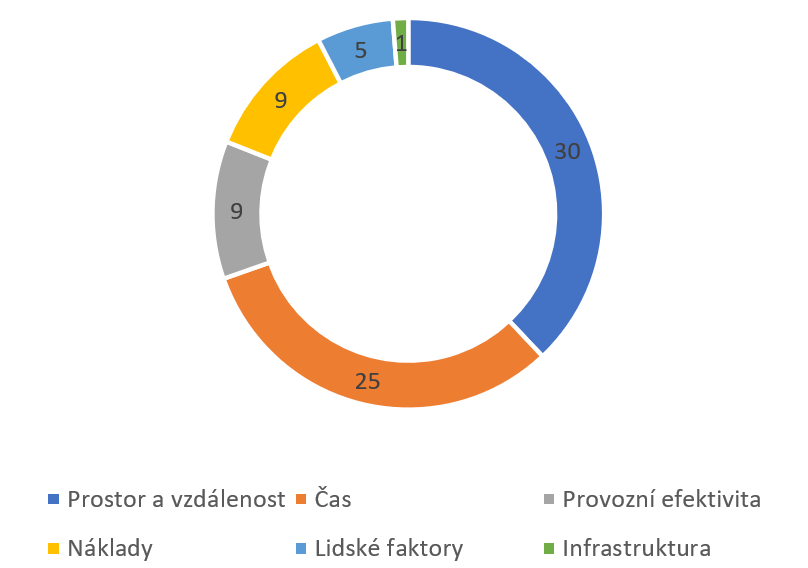
\includegraphics[width=1\textwidth]{figures/slap_ea/pristupyReseniSlapGraf.png}
        \caption{Graf udávající optimalizační kritéria pro řešení SLAP v odborné literatuře a jejich četnost. Vytvořeno na základě dat~z~\cite{slapReview}.}
        \label{fig:grafPristupy}
    \end{minipage}\hfill
    \begin{minipage}{0.49\textwidth}
        \centering
        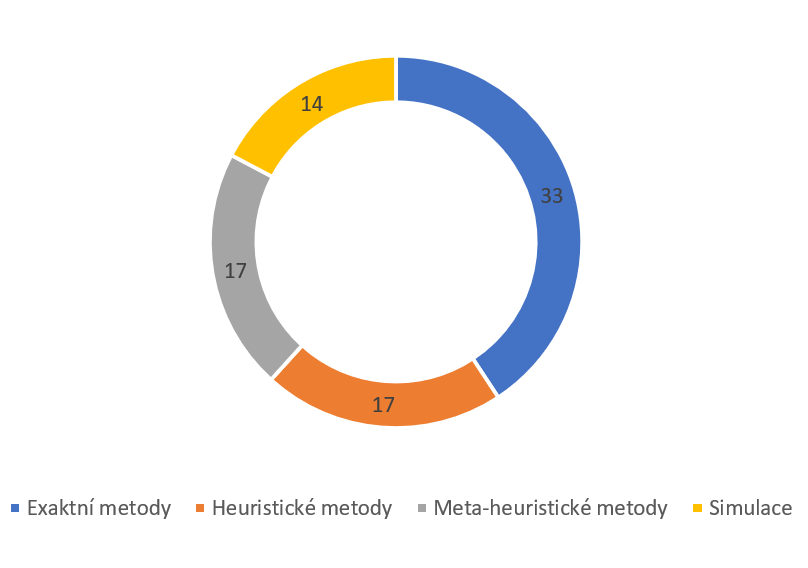
\includegraphics[width=1\textwidth]{figures/slap_ea/vykonnostniMeritkoGraf.png}
        \caption{Graf udávající optimalizované výkonnostní indikátory (KPI) skladu v odborné literatuře a jejich četnost. Vytvořeno na základě dat~z~\cite{slapReview}.}
        \label{fig:grafMeritka}
    \end{minipage}\hfill
\end{figure*}

V práci~\cite{slapSeacomp} autoři implementovali nástroj pro minimalizaci času zpracování objednávek. Práce řeší problém SLAP pomocí seřazení produktů od nejčastěji kupovaného po nejméně kupovaný a slotů lokací od nejbližšího k vchodu a východu ze skladu až po ten nejvzdálenější. Následně provádí namapování produktů do slotů tak, že nejčastěji kupovaný produkt je v nejvýhodnějším slotu, atd. Následně byl nástroj vyhodnocen na modelu existujícího skladu a bylo zjištěno, že časy manipulace s materiálem byly zredukovány o $37.8\%$ oproti původnímu stavu. Tento princip byl pro porovnání využit i~v~této práci a lze jej vidět v~grafu \ref{fig:vyhodnoceniGrafTrain} jako \texttt{Battista a spol}. Při experimentech v této práci dosáhl zlepšení $33.2\%$.

Genetický algoritmus pro minimalizaci ujeté vzdálenosti ve skladu byl použit v~práci~\cite{optimisationOrderPickingGA}. Autoři optimalizovali přesně definovaný model skladu daný zákazníkem popsaný matematickou funkcí, a podařilo se jim snížit cestovanou vzdálenost ve skladu při zpracovávání objednávek o $28\%$. To vede ke značnému zrychlení pickování.

Řešení problematiky SLAP pomocí meta-heuristického přístupu založeného na genetických algoritmech se objevilo také v práci~\cite{slapPickAndPass}. Byla zde vytvořena matematická objektivní funkce, která přesně popisovala rozložení skladu. V této práci autoři počítali také s doplňováním produktů a soustředili se na zjištění důležitosti rozložení zátěže mezi jednotlivé pickery, které je dle nich esenciální pro správnou optimalizaci.

Autoři práce~\cite{whModelSim} se kvůli složitosti a možnému zavedení chyb či ignorování přepisu skladu na matematickou funkci rozhodli využít pro vyhodnocení simulátor skladu. Autoři zmiňují, že ze všech možných kombinací druhů simulace skladu je nejvhodnější a nejpřirozenější simulace pomocí diskrétních událostí, protože sklad je v podstatě kolekce entit, které reagují na fixní události (jako je například pickování objednávek). Dále byla v rámci práce provedena případová studie existujícího skladu a implementován simulátor daného skladu. Výsledkem každé simulace byl soubor obsahující veškeré KPI skladu, které mohli být dále jednoduše použity pro srovnávání a podařilo značně zvýšit množství uložených produktů.

Heuristický přístup byl použit v práci \cite{exactTimeSlap}. Byl vytvořen komplexní matematický model skladu a pomocí celo-číselného programování byl optimalizován čas cesty po skladu. V práci byl implementován heuristický vyhledávací algoritmus tabu a pro malé problémy nalezl algoritmus vždy optimální řešení.

Podobně jako ve zmíněných pracích je i zde experimentováno se základním i genetickým přístupem. Navíc je práce doplněna i o jiné optimalizace a umožňuje uživateli nastavit si vlastní sklad a strukturu objednávek, všechno v rámci grafické aplikace.



\chapter{Evoluční algoritmy}
\label{EA}
Tato kapitola pojednává o obecném popisu heuristických vyhledávacích a optimalizačních algoritmů inspirovaných přírodou. Jmenovitě se jedná o genetické algoritmy, diferenční evoluci, optimalizaci rojem částic a algoritmus umělých včelstev. Na konci je v krátkosti popsán známý kombinatorický problém obchodního cestujícího a jsou popsány redefinice výše zmíněných evolučních algoritmů pro tento problém řešený v diskrétním prostoru s několika omezujícími podmínkami.

%%%%%%%%%%%%%%%%%%%%%%%%%%%%%%%%%%%%%%%%%%%%%%%%%%%%%%%%%%%%%%%%%%%%%%%%%%%%%%%%%%%%%%%%%%%%%%%%%%%%%%%%%%%%%%%%%%%%%%%%

\section{Genetické algoritmy}
Při studiu genetických algoritmů (ang. \emph{Genetic Algorithms} -- zkratka GA) jsem vycházel z prací~\cite{GAoptimisModel, GAstudy, introductionEvo, optimisationOrderPickingGA}. Genetické algoritmy jsou heuristické vyhledávací nebo optimalizační algoritmy inspirované Darwinovským principem evoluce skrze přirozený výběr. Genetický algoritmus však funguje na vysoké úrovni abstrakce evolučních procesů za účelem \uv{evoluce} řešení pro zadané problémy. Snaží se optimalizovat (tedy minimalizovat či maximalizovat) objektivní funkci, a to za pomoci přechodu z jedné sady chromozomů na novou a to za pomoci genetických operátorů. Genetické algoritmy byly vytvořeny Johnem Hollandem v~roce 1970 za účelem nalezení řešení problémů, které byly výpočetně neřešitelné. Po uvedení se dočkaly velké popularity a rychlého vývoje a byly aplikovány k řešení celé řady problému v různých odvětví jako je věda či průmysl. V dnešní době jsou genetické algoritmy stále velmi aktivní a rostoucí oblast výpočetní inteligence, kam patří mimo jiné například také umělé neuronové sítě~\cite{GAoptimisModel}.

Každý genetický algoritmus pracuje nad populací umělých chromozomů (chromozom je také označován jako jedinec populace), kde každý chromozom představuje jedno řešení problému. Chromozom je konečný řetězec (často binární) a má hodnotu \emph{fitness}, což je desetinné číslo, které udává jak dobrý daný chromozom je. Na začátku výpočtu se provádí inicializace populace, kde se pomocí uniformní náhodné funkce vygenerují hodnoty pro každého jednotlivce v populaci. Dále genetický algoritmus provádí selekci a kombinaci jednotlivců, založenou na velikosti jejich hodnoty \emph{fitness} (dle toho zda se jedná o minimalizační či maximalizační problém), za účelem vytvoření nové generace populace, která bude poskytovat lepší řešení daného problému. Tento proces přirozeného výběru je opakován a nové generace jsou vytvářeny až do chvíle, kdy je splněno kritérium pro zastavení (nalezení optimálního řešení nebo dosažení jistého počtu iterací)~\cite{GAoptimisModel}.

\subsection{Struktura genetických algoritmů}
Genetický algoritmus je velmi modulární (skládá se z několika odlišných částí), což umožňuje znovupoužití jednotlivých částí v jiných genetických algoritmech, usnadňující jejich implementaci. Hlavní části genetického algoritmu jsou kódování genů a chromozomů, fitness funkce (objektivní funkce), křížení jedinců (ang. \emph{crossover}), mutace (ang. \emph{mutation}) a~selekce do další generace na základě fitness funkce, jak lze vidět na obrázku \ref{fig:gaWorkflow}. Za pomoci těchto operátorů genetický algoritmus hledá vhodnější řešení pomocí evoluce a to skrze navazující iterace zvané jako generace~\cite{GAoptimisModel, introductionEvo}.

\begin{figure}[t]
    \centering
    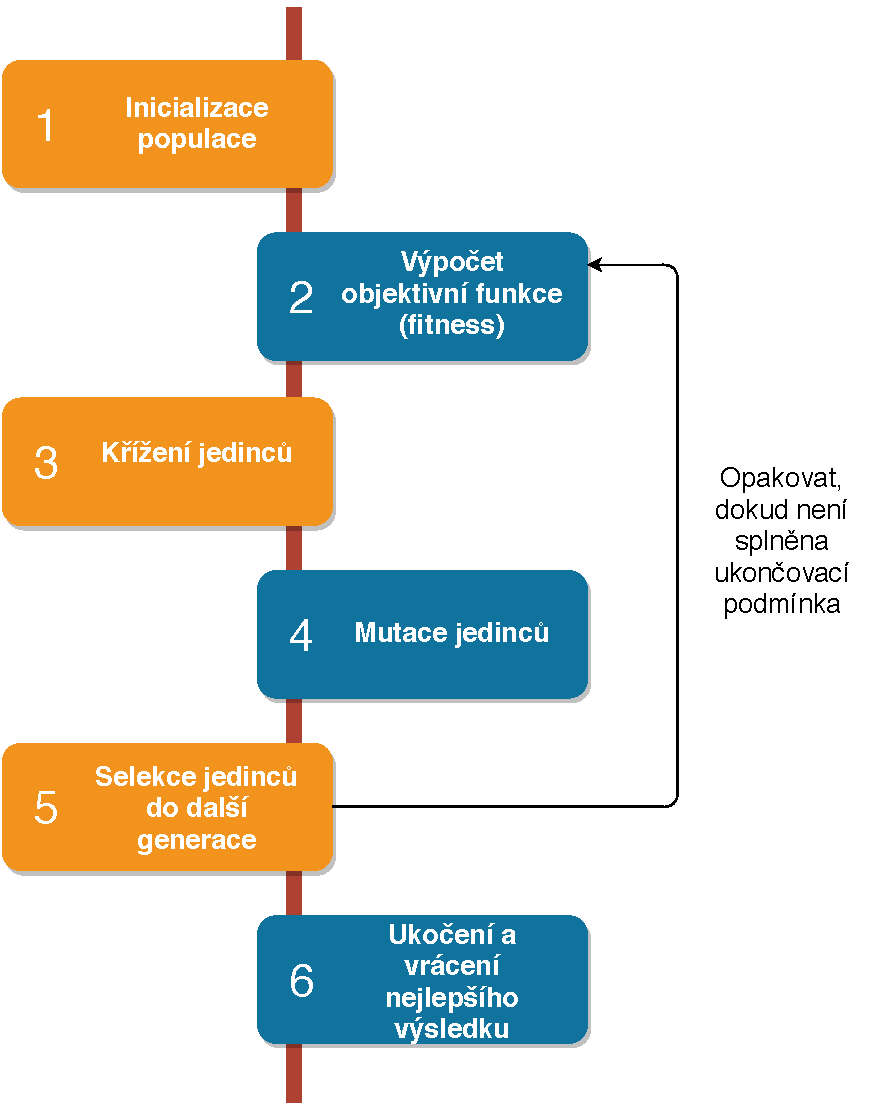
\includegraphics[width=0.50\linewidth]{figures/slap_ea/geneticky_algoritmus.pdf}
    \caption{Princip výpočtu genetického algoritmu. Vytvořeno na základě dat z~\cite{GAoptimisModel}.}
    \label{fig:gaWorkflow}
\end{figure}

\subsubsection{Kódování chromozomů a genů}
Jak již bylo zmíněno, genetický algoritmus modifikuje populaci chromozomů za účelem dosažení lepších jedinců. Chromozomy jsou abstrakcí DNA chromozomů a jsou reprezentovány jako řetězce (často binární), které představují řešení daného problému. Jednotlivé části chromozomu jsou v literatuře nazývány geny a chromozom je tedy řetězec genů určité (konečné) délky. Pozice genu v chromozomu je typicky označována jako \emph{locus}. Hodnota, které gen nabývá se nazývá \uv{\emph{allele}} hodnota. Řešený problém je vždy takzvaně \uv{zakódován} do chromozomů a interpretace této kódované reprezentace se liší problém od problému. Toto je jedna z hlavních výhod genetických algoritmů, a to sice že podobné reprezentace lze použít pro množství různých problémů, umožňující vývoj společných modulů a usnadňující aplikaci genetických algoritmů na nové, zatím neřešené problémy~\cite{GAoptimisModel, introductionEvo}.

\subsubsection{Fitness funkce}
Fitness funkce (objektivní funkce) je výpočetní prostředek, který slouží pro ohodnocení kvality chromozomu vzhledem k jeho schopnosti řešit daný problém, což mimo jiné určuje také pravděpodobnost, s jakou bude daný chromozom vybrán do další generace. Optimální hodnota této funkce se bude lišit v závislosti na řešeném problému, zda se jedná o minimalizační čí maximalizační úlohu. Fitness funkce je opět závislá na řešeném problému a~úzce spojena s kódováním chromozomu, protože značná část interpretace (významu) chromozomu je zakódovaná právě do této fitness funkce~\cite{GAoptimisModel}. 

\subsubsection{Selekce jedinců}
\label{selekceGA}
Selekční operátor slouží pro usměrňování evoluce chromozomů. Do další generace je z populace vybrán jen stanovený počet jedinců, a to, kteří jedinci budou vybráni, závisí zejména na hodnotě fitness jednotlivých prvků (což je diskriminátor kvality jedinců) a z části také na zvoleném selekčním algoritmu. Za účelem zachování diverzity nejsou z populace zpravidla vybráni jen ti nejvhodnější jedinci, ale i jedinci s horší hodnotou fitness (tzn. ne tak dobrá řešení). Jedinci s lepší fitness však můžou být zvýhodňováni, aby nebyl výběr čistě náhodný, ale do další generace se tak dostaly pravděpodobněji ta lepší řešení. Selekce se často provádí s nahrazováním, tzn. lepší chromozomy mohou vybrány vícekrát a dokonce být kombinovány sami se sebou. Zde je přehled několika nejznámějších selekčních metod~\cite{GAoptimisModel, introductionEvo, GAstudy}:

\begin{figure}[t]
    \centering
    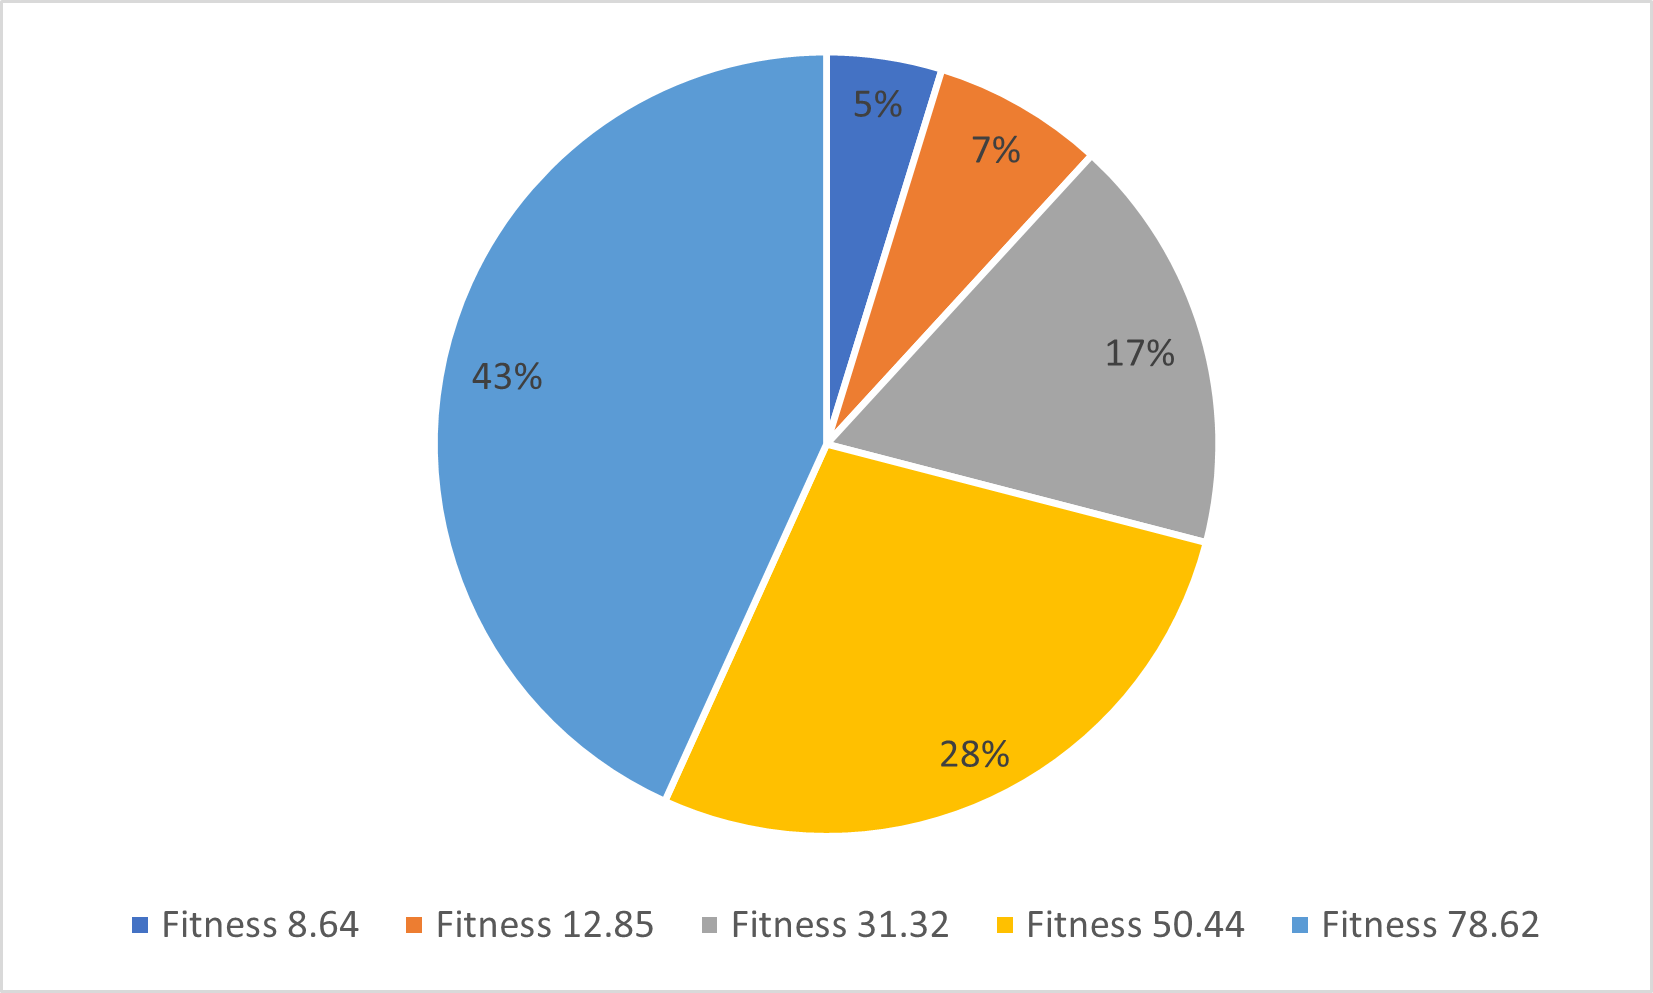
\includegraphics[width=0.9\linewidth]{figures/slap_ea/Roulette.png}
    \caption{Vizualizace příkladu selekce pomocí metody ruleta s pěti jedinci, každý s~různou hodnotou fitness. Největší šanci ($43\%$) na výběr do další generace populace má jedinec s hodnotou fitness $78.62$.}
    \label{fig:roulette}
\end{figure}

\begin{itemize}
    \item \textbf{\emph{Roulette wheel method}} (metoda rulety) -- Je to jedna z nejpoužívanějších metod pro selekci v genetických algoritmech. Zde pravděpodobnost, že bude chromozom vybrán do další generace odpovídá proporčně hodnotě fitness tohoto chromozomu. Tzn. že pravděpodobnost je vypočtena jako hodnota fitness daného chromozomu děleno suma hodnoty fitness všech chromozomů v populaci. V případě, že se jedná o minimalizační problém, by se častěji vybíraly horší řešení, proto je nutné před provedením této metody invertovat hodnoty fitness jednotlivých chromozomů (viz příklad \ref{fig:roulette}).
    \item \textbf{\emph{Rank method}} (metoda \uv{pořadí}) -- Tato metoda v podstatě funguje na stejném principu jako metoda rulety, avšak odstraňuje její největší problém. Metoda rulety má problémy v případě, že hodnota fitness jednotlivých prvků se hodně liší (tzn. pokud jeden chromozom bude zabírat většinu rulety, ostatní nemají téměř žádnou šanci na výběr). Metoda řeší zmíněný problém tak, že seřadí všechny chromozomy na základě jejich fitness, a postupně jim přiřazuje čísla od $1$ po $N$. Tzn. nejvhodnější chromozom bude mít hodnotu $N$, zatímco nejméně vhodný chromozom bude mít hodnotu $1$. Vzhledem k tomu, že tato metoda nezvýhodňuje lepší řešení tak výrazně, má pomalejší konvergenci.
    \item \textbf{\emph{Elittism method}} (\uv{elitní} metoda) -- V době, kdy se vytváří nová generace populace, rovnou překopíruje nejlepší (nebo několik) řešení. To zaručí že algoritmus neztratí nejlepší nalezené řešení, což výrazně zrychluje konvergenci genetického algoritmu.
    \item \textbf{\emph{Tournament metod}} (metoda turnaje) -- Metoda vybere dva (obecně $N$) chromozomů a vybere ten s nejvyšší hodnotou fitness.
    \item \textbf{\emph{Truncation method}} (metoda \uv{zkrácení}) -- Tato metoda vybere z populace náhodně jeden chromozom (s uniformním rozložením pravděpodobnosti).
\end{itemize}


\subsubsection{Křížení jedinců}
\label{krizeniGA}
Vytváření nových jedinců (následníci rodičů) do další generace je v genetických algoritmech prováděno za pomoci sady před-definovaných operátorů. Tyto operátory na vstupu přijímají dva jedince z aktuální generace (rodiče) a produkují na výstup dva nové jedince (potomky). Biologická analogie je kombinování genetického materiálu (DNA), jež se projevuje při reprodukci živočichů. Vzhledem k tomu, že ve většině případů jsou jedinci pro křížení vybírání na základě jejich fitness hodnoty, je pravděpodobné že jejich kombinací vznikne lepší chromozom. Operátor křížení je ve své podstatě nedeterministický, protože se provádí pouze s~určitou pravděpodobností. Také výsledek tohoto operátoru je nedeterministický, protože je založen na stochastické funkci. Operátor křížení má jeden parametr, a to je tzv. \emph{crossover rate}, reprezentující jak často se bude křížení provádět. Při potencionálním křížení se tedy vygeneruje číslo v intervalu $[0,1]$ s uniformním rozložením, pokud je hodnota \emph{crossover rate} vyšší než vygenerované číslo, tak se křížení provede, jinak nikoli. Zde je přehled několika nejznámějších operátorů křížení~\cite{GAoptimisModel, GAstudy}:

\begin{itemize}
    \item \textbf{\emph{One-point crossover}} (operátor křížení jednoho bodu) -- S uniformní pravděpodobností se náhodně vybere číslo $k$ z intervalu $1$ až $N$, kde $N$ je délka chromozomu. Poté se vytvoří potomci takto: První potomek obsahuje řetězec genů $0$ až $k$ z prvního rodiče a zbytek z druhého rodiče. Druhý potomek obsahuje řetězec genů $0$ až $k$ z druhého rodiče a zbytek z prvního rodiče.
    \item \textbf{\emph{Two-point crossover}} (operátor křížení dvou bodů) -- Funguje na stejném principu jako předchozí operátor, ale místo jednoho bodu vybírá dva náhodné body. Potomci poté nesestávají z jedné části z jednoho rodiče a z jedné části z druhého rodiče, nýbrž ze dvou částí z jednoho rodiče a jedné (prostřední) části z druhého rodiče. Tento operátor lze obecně použít na $N$ bodů (\emph{N-point crossover}).
    \item \textbf{\emph{Uniform crossover}} (uniformní operátor křížení) -- Vytváří potomky tak, že prochází rodiče a na každé pozici uniformě vybírá rodiče, ze kterého se použije hodnota allele.
\end{itemize}


\subsubsection{Mutace jedinců}
\label{mutaceGA}
Oproti operátoru křížení, který na základě dvou rodičů vytváří dva potomky, operátor mutace upravuje pouze jednoho jedince. Tyto změny jsou typicky malé, jsou prováděny náhodně a jsou typicky prováděny až po procesu křížení jedinců. Podobně jako u křížení, je i zde definován operátor udávající pravděpodobnost, s jakou bude jedinec mutován (ang. \emph{mutation rate}). Tento operátor funguje stejně jako operátor uvedený u křížení jedinců. Dále je ale definována pravděpodobnost mutace jednotlivých genů. Pravděpodobnost mutace bývá však relativně malá, obzvláště ve srovnání s pravděpodobností křížení. Lze provést například pomocí invertování bitů v binárním řetězci~\cite{GAoptimisModel, GAstudy}.


\subsubsection{Proces evoluce}
Jak již bylo zmíněno, na počátku evoluce je celá populace (všichni jedinci) náhodně inicializovaná. Následně je vyhodnocena fitness funkce pro každý chromozom. Následně se pomocí genetických operátorů vytváří nová generace následníků. Tento proces se skládá z~několika částí, které jsou detailněji popsány výše. První je proveden proces výběru jedinců pro mutování. Takto vybraní jedinci jsou kříženi mezi sebou. Z tohoto procesu vznikne stejný počet potomků, jako do něj vstupuje rodičů a následně jsou někteří z jedinců mutováni. Tito jedinci vstupují do další iterace jako nová generace. Takovýto proces vytváření nových generací je opakován až do doby, kde je buďto splněna podmínka optimalizace/hledání (např. splnění všech podmínek), nebo je dosažen maximální počet generací. Existuje množství různých schémat, jak může genetický algoritmus fungovat. Zde je příklad několika nejběžnějších~\cite{GAoptimisModel, introductionEvo}:

\begin{itemize}
    \item \textbf{Úplné nahrazení} -- V tomto schématu jsou po každé iteraci nahrazeni pomocí genetických operátorů všichni jedinci svými následníky.
    \item \textbf{Ustálené schéma} -- Nová generace je vytvořena generováním jednoho nového následníka každou generaci, který nahrazuje nejméně vhodného jedince předchozí populace.
    \item \textbf{Nahrazení s elitní částí} (nejrozšířenější použití) -- Téměř úplné nahrazení jedinců do další generace (skrze genetické operátory), ale jeden nebo dva jedinci (s nejlepší hodnotou fitness) jsou přesunuti beze změny. Toto schéma zaručuje, že nebudou ztraceny doposud nejlepší výsledky skrze nedeterministický (náhodný) výběr.
\end{itemize}

\begin{table}[htp]
\centering
\caption{Shrnutí genetických algoritmů. Převzato z~\cite{introductionEvo}.}
\label{tab:GA}
\begin{tabular}{|l|l|}
\hline
Reprezentace & Různé druhy, např. bitové řetězce \\ \hline
Křížení & Různé druhy, např. jednobodové křížení \\ \hline
Mutace & Různé druhy, např. inverze bitů \\ \hline
Selekce rodičů & V závislosti na fitness (např. metoda rulety) \\ \hline
Selekce následníků & Generační (následník nahrazuje rodiče) \\ \hline
\end{tabular}
\end{table}


%%%%%%%%%%%%%%%%%%%%%%%%%%%%%%%%%%%%%%%%%%%%%%%%%%%%%%%%%%%%%%%%%%%%%%%%%%%%%%%%%%%%%%%%%%%%%%%%%%%%%%%%%%%%%%%%%%%%%%%%

\section{Diferenční evoluce}
Při studiu diferenční evoluce (ang. \emph{Differential Evolution} -- zkratka DE) jsem vycházel z~\cite{DE_GA_TSP, introductionEvo}. Diferenční evoluce v teorii vychází z genetického algoritmu. Je založena na populaci jedinců a umožňuje provádět tři typy operací s jedinci, a sice: křížení, mutaci a selekci do další generace. Tato metoda je používána k optimalizaci nelineárních funkcí ve spojitém prostoru a pracuje tedy s reálnými čísly. Populace je tvořena jedinci (kandidátní řešení), reprezentovanými vektory reálných čísel $\bar{x} \in \mathbb{R}^n$, v diferenční evoluci také nazývaných jako cílové vektory. Populace je na začátku náhodně inicializována, je vypočtena hodnota fitness pro každého jedince a poté je prováděna optimalizace. Odlišujícím faktorem je že pořadí jedinců v populaci nezávisí na jejich hodnotě fitness a odklonění od použití klasických operátorů evolučních algoritmů~\cite{DE_GA_TSP, introductionEvo}.

\subsubsection{Mutace}
Algoritmus používá tzv. diferenční mutaci, kde nové kandidátní řešení $\bar{v}'$ je získáno přičtením vektoru váženého rozdílu dvou náhodně vybraných jedinců populace:

\begin{align}
    \label{eq:DE1}
    \bar{v}' = \bar{v} + F (\bar{a} - \bar{b}),
\end{align}
kde $F$ reprezentuje faktor škálování, což je reálné číslo, které slouží pro kontrolu rychlosti evoluce. Hodnoty $\bar{a}$ a $\bar{b}$ jsou již zmínění dva náhodně vybraní jedinci populace. Dalším operátorem je operátor křížení, který slouží ke zvýšení diverzity populace~\cite{introductionEvo}.

\subsubsection{Křížení}
V diferenční evoluci se používá uniformní křížení s parametrem $C_r \in \interval[{0,1}]$, který udává pravděpodobnost, s jakou bude (pro jakoukoli pozici v aktuálním rodiči) hodnota \emph{allele} rodiče zahrnuta do potomka, oproti křížení v genetických algoritmech, kde pravděpodobnost udává zda budou daní rodiče vůbec kříženi, či nikoli. Nový cílový vektor $\bar{x}'$ je získán křížením následovně:

\begin{align}
    \label{eq:DE2}
    \bar{x}_k' = \begin{cases}
               \bar{v}_k, & \text{pokud } (U \leq C_r) \lor (j = k) \\
               \bar{x}_k, & \text{jinak}.
               \end{cases}.
\end{align}
Hodnota $U \in \interval[{0,1}]$ označuje náhodně vygenerované reálné číslo. Hodnota $j$ je parametr, který zaručuje, že se potomek bude lišit alespoň jedním \emph{allele} a nakonec hodnota $k$ slouží pro iterování skrze jednotlivé hodnoty \emph{allele}~\cite{DE_GA_TSP}.

\subsubsection{Selekce}
Selekce porovnává fitness nového cílového vektoru (mutovaného a kříženého) s původním. Do další generace je vybrán ten vektor, který má lepší hodnotu fitness:

\begin{align}
    \label{eq:DE3}
    \bar{x} \leftarrow \bar{x}', \text{ pokud } f(\bar{x}') \geq f(\bar{x}),
\end{align}
kde $f$ představuje objektivní funkci pro maximalizační optimalizační problém~\cite{DE_GA_TSP}.

Diferenční evoluce má spoustu variací, např. se liší způsoby jak lze vybírat rodiče. V~literatuře se používá zavedená notace \texttt{DE/x/y/z}, kde \emph{x} reprezentuje výběr rodiče (např. \uv{rand} -- nádhoný rodič, \uv{best} -- nejlepší rodič), \emph{y} je počet diferenčních vektorů a \emph{z} značí použité schéma křížení (např. \uv{bin} je uniformní křížení)~\cite{introductionEvo}.



\begin{table}[htp]
\centering
\caption{Shrnutí diferenční evoluce. Převzato z~\cite{introductionEvo}.}
\label{tab:DE}
\begin{tabular}{|l|l|}
\hline
Reprezentace & Vektor reálných čísel \\ \hline
Křížení & Uniformní křížení\\ \hline
Mutace & Diferenční mutace \\ \hline
Selekce rodičů & \texttt{DE/rand/1/bin} -- náhodně, \texttt{DE/best/1/bin} -- nejlepší, ... \\ \hline
Selekce následníků & Deterministické nahrazení (rodič vs. potomek) \\ \hline
\end{tabular}
\end{table}


%%%%%%%%%%%%%%%%%%%%%%%%%%%%%%%%%%%%%%%%%%%%%%%%%%%%%%%%%%%%%%%%%%%%%%%%%%%%%%%%%%%%%%%%%%%%%%%%%%%%%%%%%%%%%%%%%%%%%%%%

\section{Algoritmus umělých včelstev}
Při studiu algoritmu umělých včelstev (ang. \emph{Artificial Bee Colony} -- zkratka ABC) jsem vycházel z~\cite{ABC, ABC_TSP}. Tento algoritmus analogicky odpovídá chování včelího hnízda a tedy používá včelařskou terminologii. V tomto algoritmu se objevují tři druhy umělých včel, a sice: \uv{zaměstnané} (ang. \emph{employed}), \uv{pozorovací} (ang. \emph{onlooker}) a \uv{průzkumné} (ang. \emph{scout}). Zaměstnaná včela navštěvuje zdroje potravy, kdežto pozorující včela vyčkává za účelem výběru zdroje potravy. Průzkumné včely provádí náhodné hledání zdroje potravy v okolí. V tomto algoritmu spadá první polovina včel do kategorie zaměstnaných, kdežto druhá polovina do kategorie pozorujících a každému zdroji potravy připadá právě jedna zaměstnaná včela. Z toho plyne, že počet zdrojů potravy je přesně roven počtu zaměstnaných včel. Průzkumnými včelami se stávají zaměstnané včely, jejichž zdroj potravy je vyčerpán zaměstnanými a pozorujícími včelami. Proces optimalizace je tedy následovný~\cite{ABC}:

\begin{enumerate}
    \item Náhodná inicializace zdrojů potravy.
    \item Umístění zaměstnaných včel na zdroje potravy v okolí.
    \item Umístění pozorujících včel na zdroje potravy v okolí.
    \item Vyslání průzkumných včel za účelem nalezení nových zdrojů potravy.
    \item Pokud není splněna ukončovací podmínka, vrácení na bod 2.
\end{enumerate}

Každá iterace algoritmu sestává ze třech fází: vyslání zaměstnaných včel na zdroje potravy v okolí a~určení množství nektaru na těchto zdrojích, výběr zdrojů potravy pozorujícími včelami po určení množství nektaru jednotlivých zdrojů a určení průzkumných včel a~jejich vyslání na možné zdroje potravy. V tomto algoritmu je kandidátní řešení problému reprezentováno jako zdroj potravy (potažmo zaměstnaná včela) a kvalitu řešení reprezentuje množství nektaru. To znamená, že čím více nektaru na zdroji potravy je, tím lepší toto řešení je. Zaměstnané a pozorující včely stochasticky modifikují zdroje potravy (řešení) a~vyhodnocují množství nektaru~(fitness). Nový zdroj potravy $v_{ij}$ je ze starého zdroje $x_{ij}$ a sousedního zdroje $x_{kj}$ vytvořen následujícím způsobem:
\begin{align}
    \label{eq:ABC1}
    v_{ij} = x_{ij} + \phi_{ij} (x_{ij} - x_{kj}),
\end{align}
kde $k \in {1, 2, ..., BN}$ a $j \in {1, 2, ... D}$ ($BN$ je počet zdrojů potravy a $D$ je dimenze řešeného problému) jsou náhodně vybrané indexy, kde však musí platit: $i \neq k$. Číslo $\phi_{ij} \in \interval[{-1,1}]$ je také generováno náhodně a slouží k určení dalšího zdroje potravy v okolí, což lze při analogii na reálnou včelu chápat jako vizuální porovnávání zdrojů potravy~\cite{ABC, ABC_TSP}.

Každý zdroj potravy si udržuje hodnotu počtu pokusů. Pokud se množství nektaru v~tomto zdroji zvýší (větší fitness hodnota), tento čítač se vynuluje. Pokud je tomu ovšem naopak a množství nektaru je nižší, tento čítač se zvýší o jedna. Pokud čítač dosáhne předem stanovené hodnoty (tzn. zdroj potravy je vyčerpán), stává se z něj průzkumná včela (tzn. zdroj je znovu náhodně inicializován a je určena jeho hodnota fitness)~\cite{ABC}.



\begin{table}[htp]
\centering
\caption{Shrnutí algoritmu umělých včelstev~\cite{ABC}.}
\label{tab:ABC}
\begin{tabular}{|l|l|}
\hline
Reprezentace & Vektor reálných čísel \\ \hline
Křížení & --- \\ \hline
Mutace & Modifikace zdrojů potravy včelami dle rovnice \ref{eq:ABC1} \\ \hline
Selekce rodičů & Náhodně vybrané zdroje potravy s omezujícími podmínkami \\ \hline
Selekce následníků & Náhodná inicializace zdroje potravy po vyčerpání nektaru \\ \hline
\end{tabular}
\end{table}


%%%%%%%%%%%%%%%%%%%%%%%%%%%%%%%%%%%%%%%%%%%%%%%%%%%%%%%%%%%%%%%%%%%%%%%%%%%%%%%%%%%%%%%%%%%%%%%%%%%%%%%%%%%%%%%%%%%%%%%%

\section{Optimalizace rojem částic}
Při studiu optimalizace rojem částic (ang. \emph{Particle Swarm Optimization} -- zkratka PSO) jsem vycházel z~\cite{PSO_GA_TSP, introductionEvo}. Tento algoritmus je inspirovaný sociálním chováním ptačího hejna, zatímco jméno a použitá terminologie odpovídá spíše fyzickým částicím. Podobně jako u~diferenční evoluce, odlišujícím faktorem je odklonění od použití klasických operátorů evolučních algoritmů a pořadí jedinců v populaci nezávisí na jejich hodnotě fitness. Optimalizace rojem částic nepoužívá operátor křížení a mutace je definována jako sčítání vektorů. Celkový přehled lze nalézt v tabulce \ref{tab:PSO}. Každé možné řešení (tzn. každý jedinec populace) $\bar{x} \in \mathbb{R}^{n}$ s sebou nese také vektor \uv{rychlostí} (ang. \emph{velocities}) $\bar{v} \in \mathbb{R}^{n}$. To znamená, že každé řešení je dvojice $\langle \bar{x}, \bar{v} \rangle$. Vektor rychlostí je později použit pro nalezení nového řešení, tzn. vektoru $\bar{x}$. Hlavní myšlenka algoritmu je tedy v tom, že nová dvojice $\langle \bar{x}', \bar{v}' \rangle$ je vytvořena z~aktuální dvojice $\langle \bar{x}, \bar{v} \rangle$, a to tak, že první se vypočte nový vektor rychlostí, a poté je přičten k řešení~\cite{introductionEvo}:

\begin{align}
    \label{eq:PSO1}
    \bar{x}' = \bar{x} + \bar{v}'.
\end{align}

Každé z řešení je tedy reprezentováno jako bod v prostoru s jistou pozicí a rychlostí, kde rychlost je použita pro výpočet následné pozice. Výpočet rychlosti samotné je v podstatě vážený součet třech komponentů, a to aktuální rychlosti a dvou vektorových rozdílů:

\begin{align}
    \label{eq:PSO2}
    \bar{v}_i = w \bar{v}_i + \phi_1 U_1 (\bar{b}_i - \bar{x}_i) + \phi_2 U_2 (\bar{c} - \bar{x}_i),
\end{align}
kde váhy $w$, $\phi_1$ a $\phi_2$ jsou označovány jako (zleva): $inertia$, faktor učení osobní změny a~faktor učení sociální změny. Hodnoty $U_1$ a $U_2$ jsou náhodně vygenerované z uniformního rozložení v intervalu $\interval[{0,1}]$. Index $i$ značí pozici v populaci/roji. Dále hodnota $\bar{b}$ označuje dosavadní nejlepší výsledek jedince populace, zatímco $\bar{c}$ označuje dosavadní nejlepší výsledek celé populace, kde první z hodnot je třeba uchovávat v paměti pro každého jedince zatímco druhou pouze pro celou populaci. Tento mechanizmus tedy vyžaduje aby jedinci byli jednoznačně identifikovatelní a měli tedy identitu, aby bylo možné upravovat jejich vlastní paměť (nejlepší dosavadní výsledek). Každého jedince populace lze tedy považovat jako trojici $\langle \bar{x}, \bar{v}, \bar{b} \rangle$, značící řešení (pozici), aktuální rychlost a dosavadní nejlepší výsledek jedince. Postup výpočtu je tedy následující~\cite{PSO_GA_TSP, introductionEvo}:

\begin{enumerate}
    \item Náhodná inicializace velikosti roje, pozic částic a rychlosti částic.
    \item Výpočet nové rychlosti částice za pomoci rovnice \eqref{eq:PSO2}.
    \item Výpočet nové pozice částice za pomoci rovnice \eqref{eq:PSO1}.
    \item Aktualizace osobních a globálního nejlepšího výsledku.
    \item Pokud není splněna ukončovací podmínka, vrácení na bod 2.
\end{enumerate}

\begin{table}[htp]
\centering
\caption{Shrnutí optimalizace rojem částic. Převzato z~\cite{introductionEvo}.}
\label{tab:PSO}
\begin{tabular}{|l|l|}
\hline
Reprezentace & Vektor reálných čísel \\ \hline
Křížení & --- \\ \hline
Mutace & Přičtení vektoru rychlostí \\ \hline
Selekce rodičů & Deterministická (rodič vytvoří jednoho následníka pomocí mutace) \\ \hline
Selekce následníků & Generační (následník nahrazuje rodiče) \\ \hline
\end{tabular}
\end{table}

%%%%%%%%%%%%%%%%%%%%%%%%%%%%%%%%%%%%%%%%%%%%%%%%%%%%%%%%%%%%%%%%%%%%%%%%%%%%%%%%%%%%%%%%%%%%%%%%%%%%%%%%%%%%%%%%%%%%%%%%

\section{$\mathcal{MAX}\!{-}\!\mathcal{MIN}$ mravenčí systém}
\label{sec:mmas}
Při studiu $\mathcal{MAX}\!{-}\!\mathcal{MIN}$ mravenčího systému (ang. $\mathcal{MAX}\!{-}\!\mathcal{MIN}$ \emph{Ant System} -- zkratka $\mathcal{MM}$AS) jsem vycházel z prací~\cite{naturalEvoAlgs, MMAS}. Tento algoritmus je, jak název napovídá, inspirovaný chováním mravenčích kolonií. Hlavní princip spočívá v nepřímé komunikaci jedinců populace reprezentujících řešení problému, zvaných mravenci. Komunikace je zajištěna analogií chemické substance zvané feromon, která je periodicky upravována jednotlivými mravenci, reprezentující kvalitu řešení. Algoritmus $\mathcal{MM}$AS je odvozen od původního algoritmu mravenčího systému (ang. \emph{Ant System}), jehož cílem je dosažení lepší výkonnosti zejména při hledání řešení komplexnějších úloh.

Jedná se o variantu mravenčího systému, která na začátku výpočtu všechny hrany inicializuje hodnotou maximální hodnotou feromonu, tedy $\tau_{max}$, což umožňuje lepší prozkoumání řešení na začátku algoritmu. Během aktualizace jsou upraveny pouze hrany, které využilo nejlepší řešení a to buď nejlepší řešení v rámci celého výpočtu nebo pouze v rámci aktuální iterace. Hodnota feromonu každé hrany $\tau_{ij}$ při aktualizaci feromonů je spočtena pomocí rovnice:

\begin{align}
    \label{eq:MMAS1}
    \tau_{ij}(t+1) = \rho \tau_{ij}(t) + \Delta \tau_{ij}^{best},
\end{align}

kde $\Delta \tau_{ij}^{best} = 1/f(s^{best})$ a $f(s^{best})$ značí cenu nejlepšího (globálního či iteračního) řešení. Množství feromonu je omezeno následovně: $\tau_{min} \leq \tau_{ij} \leq \tau_{max}$. Toto omezení je zavedeno kvůli relativně vysoké pravděpodobnosti brzké stagnace vyhledávání způsobené značným důrazem na prohledávání založeném zejména na nejlepším řešení, tzn. aby rozdíly mezi množstvím feromonů jednotlivých hran nebyly příliš obrovské. Dále tento algoritmus často obsahuje opakovanou inicializaci feromonů všech hran hodnotou $\tau_{max}$ ve chvíli, kdy je detekována stagnace vyhledávání. Tento krok do procesu vyhledávání zavede dostatečné množství diverzity, aby se předcházelo stagnaci vyhledávání.

Pokud je pro aktualizaci feromonů použito vždy globální nejlepší řešení, hledací proces se může velmi rychle zaseknout v lokálním minimu a limitovat prohledávání lepších řešení, což může vést ke špatným výsledkům. Riziko uváznutí v lokálním minimu je sníženo, pokud se pro aktualizaci používá nejlepší řešení v rámci iterace, protože to se může značně lišiti každou iteraci a tedy lze dosáhnout diverzity a lepšího prohledávání prostoru. Tyto dva přístupy je ovšem možné také kombinovat.

%%%%%%%%%%%%%%%%%%%%%%%%%%%%%%%%%%%%%%%%%%%%%%%%%%%%%%%%%%%%%%%%%%%%%%%%%%%%%%%%%%%%%%%%%%%%%%%%%%%%%%%%%%%%%%%%%%%%%%%%

\section{Redefinice jednotlivých metod pro diskrétní prostor}
\label{section:redefiniceTSP}
Téměř všechny evoluční algoritmy popsané v této kapitole pracují implicitně ve spojitém prostoru -- tzn. počítají s reálnými čísly. Některé problematiky, jako je například problém obchodního cestujícího nebo problém distribuce a alokace produktů do lokací ve skladu pracují v diskrétním prostoru a tedy počítají s celými čísly. Aby bylo možné evoluční algoritmy na tyto problémy aplikovat, je potřeba provést redefinici algoritmu a s tím související redefinici jeho operátorů (mutace, křížení, ...). V této kapitole bude krátce popsán problém obchodního cestujícího a redefinice jednotlivých metod (vyjma mravenčího algoritmu), aby byly schopny řešit tento problém v diskrétním prostoru. V následujících sekcích je typicky popsáno jen nutné minimum pro fungování v diskrétním prostředí a k řešení problému obchodního cestujícího -- velká část z algoritmů zůstává stejná jako u spojitých verzí algoritmů popsaných dříve v kapitole a tedy zde už není popisována. Důvod, proč je zde tato podkapitola je, že problém obchodního cestujícího je v literatuře velmi často řešeným problémem a~má mnoho společného s problémem řešeným v rámci této práce -- problematikou distribuce a alokace produktů do lokací ve skladu, která je v této práci řešena právě pomocí těchto redefinic evolučních algoritmů.

\subsection{Problém obchodního cestujícího}
\label{section:TSP}
Tento problém by se dal popsat následovně: pokud chce obchodní cestující navštívit každé z $m$ měst právě jednou (kde délka cesty z města $i$ do města $j$ je označována jako $c_{ij}$) a následně se vrátit do počátečního města, jaká je nejkratší taková cesta? Problém obchodního cestujícího spadá do třídy NP-úplných problémů. To znamená, že pokud existuje efektivní řešení (takové, že řeší daný problém v polynomiálním čase) problému obchodního cestujícího, pak existuje efektivní řešení pro každý problém z třídy NP-úplných problémů. Pro formulaci tohoto problému se používá graf $G = (V,E)$, kde $V \in {1,2, ... N}$ jsou uzly reprezentující města a $E$ hrany reprezentující cesty mezi nimi. Každá hrana má cenu, která reprezentuje vzdálenost mezi těmito městy, tzn. čím větší cena hrany, tím delší je cesta mezi těmito městy. Pokud se obchodní cestující může dostat z každého města do kteréhokoli jiného města, pak je graf úplný. Okružní výlet se skládá z jisté podmnožiny uzlů a hran, zvaný obecně jako cesta či v teorii grafů jako Hamiltonova kružnice. Výsledkem algoritmů řešící tento problém je tedy sekvence délky počtu měst s nejnižší cenou (nejkratší cestou), kde se žádné z měst neopakuje a každé sousední město musí být dosažitelné skrze jednu hranu~\cite{TSP, ABC_TSP}.


\subsection{Redefinice genetických algoritmů pro diskrétní prostor}
Při studiu jsem vycházel z~\cite{GA_TSP, orderedCrossover}. Řešení problému obchodního cestujícího (individuum z~populace nebo také chromozom) lze chápat jako cestu složenou z pole genů, kde každý gen reprezentuje jedno město. Město lze reprezentovat například pomocí celočíselného identifikátoru města nebo jeho souřadnic ve formě $(x, y)$. Populace, selekce a fitness fungují na stejném principu jako ve spojitém prostoru, není je tedy potřeba předefinovávat. Je však nutné redefinovat operátory křížení a mutace tak, aby neprodukovaly v řešení duplicitní hodnoty.

\paragraph{Ordered crossover} (česky uspořádané křížení) je křížení, které neporušuje omezení problému obchodního cestujícího specifikované v části \ref{section:TSP}. To znamená že po zkřížení dvou rodičů, potomek bude stále validním řešením a tedy bude obsahovat všechna města a žádné z nich se nebude opakovat. Princip je takový, že pro vytvoření potomka se vybere jedna či více částí cesty z prvního z rodičů. Následně jsou doplněny chybějící města z druhého rodiče a to v takovém pořadí, v jakém se nachází v druhém rodiči. Druhý potomek je vytvořen úplně stejným principem, pouze se role rodičů obrací. Příklad aplikace tohoto operátoru je graficky znázorněn na obrázku \ref{fig:orderedCrossover}.

\begin{figure}[t]
    \centering
    \tmpframe{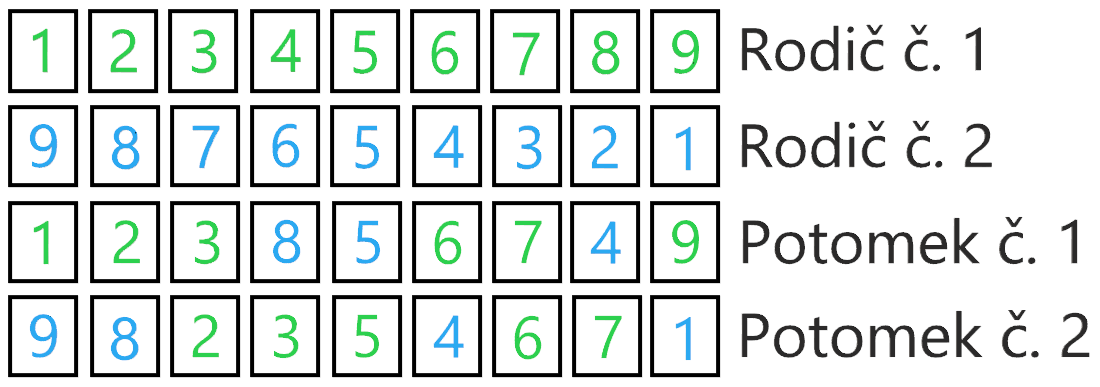
\includegraphics[width=0.7\linewidth]{figures/slap_ea/OrderedCrossover.png}}
    \caption{Graficky znázorněný příklad uspořádaného křížení dvou rodičů~\cite{orderedCrossover}.}
    \label{fig:orderedCrossover}
\end{figure}

\paragraph{Ordered mutation} (česky uspořádaná mutace) je mutace, která obdobně jako uspořádané křížení neporušuje žádné z omezení problému obchodního cestujícího. Funguje na jednoduchém principu přemístění prvku z pozice $A$ na pozici $B$, kde platí, že $A \neq B$. Na tuto mutaci existují různé variance, jako například prohození prvků na indexech $A$ a $B$, či inverze části cesty.


\subsection{Redefinice diferenční evoluce pro diskrétní prostor}
V této sekci je popsána tzv. SBDE -- \emph{step-based differential evolution} (česky volně přeloženo jako \uv{diferenční evoluce založená na krocích}. V této verzi jsou všechny potřebné aritmetické operátory redefinovány následovně~\cite{DE_GA_TSP}:

\paragraph{Element}
Element $(x,y)$ reprezentuje hranu $(x,y)$ mezi městy $x$ a $y$.

\paragraph{Jedinec}
Kandidátní řešení, skládá se z elementů a představuje Hamiltonskou kružnici.

\paragraph{Operátor násobení}
$rand \in \interval[{0,1}] \times \text{element}$ = $rand \in \interval[{0,1}] \times (x,y)$ udává, že element $(x,y)$ bude pro konstrukci nového kandidátního řešení (individua) použit s pravděpodobností $rand$. Při řešení problému obchodního cestujícího výraz $0.3 \times (1,2)$ říká, že hrana $(1,2)$ bude při konstrukci nové cesty navštívena s pravděpodobností $0.3$.

\paragraph{Operátor odečítání}
Pokud $x1$ a $x2$ jsou jedinci populace, potom výraz $x1 - x2 = e \text{ } | \text{ } e \in x1 \land e \not\in x2$, tzn. výsledkem jsou všechny hrany, které jsou v $x1$ a zároveň nejsou v $x2$.

\paragraph{Operátor sčítání}
Pokud se element nachází v obou jedincích, element je použit ve výsledku, a je použita vyšší z pravděpodobností daných elementů se vyskytovat v kandidátním řešení. Pokud se prvek nachází pouze v jednom z dvou řešení, je použit ve výsledku a to se stejnou pravděpodobností.

\paragraph{Výpočet}
\label{binomicalCrossover}
Redefinice aritmetických operátorů pro diskrétní prostor s jistým významem pro řešení problému obchodního cestujícího umožňuje použití binomického křížení, které se vyskytuje v klasické diferenční evoluci. Operátor mutace je třeba trochu upravit, a to následovně:

\begin{align}
    \label{eq:SBDE1}
    \bar{v} = \omega \times x_a + r_{rand} \times (x_b - x_c),
\end{align}

kde $\omega$ a $r_{rand}$ jsou pravděpodobnosti a jsou generovány náhodně pro každý element. V každé iteraci je pro každého jedince náhodně vygenerováno $\alpha \in \interval[{0,1}]$. Každý element v~jedinci, který nemá pravděpodobnost nižší než je hodnota $\alpha$, je umístěn do \uv{sady zbytků}. Z této sady zbytků se poté berou elementy pro konstrukci kandidátního řešení, Hamiltonské kružnice. V případě, že kandidátní řešení ještě není úplné a sada zbytků je již prázdná, je provedeno heuristické vyhledání k doplnění kandidátního řešení (např. hledání nejbližšího souseda). Zbytek je již stejný jako v klasické verzi diferenční evoluce.


\subsection{Redefinice algoritmu umělých včelstev pro diskrétní prostor}
V této sekci je popsáno řešení problému obchodního cestujícího pomocí algoritmu umělých včelstev založeného na \emph{swap sequence} (česky volně přeloženo jako \uv{sekvence výměny}) a~\emph{swap operators} (česky operátory výměny). Ty jsou definovány následovně~\cite{ABC_TSP}:

\paragraph{Operátor výměny}
Pokud $X$ je možné řešení problému, tedy sekvence měst, kterými musí obchodní cestující projít -- Hamiltonská kružnice $X = (x1, x2, ... x_n, x1)$ s množinou měst $V = {1,2, ... N}$, kde $x_i \in V$ a $x_i \neq x_j, \forall i \neq j$, pak je operátor výměny $SO(i,j)$ definován jako výměna měst/uzlů $x_i$ a $x_j$ v možném řešení problému $X$. Symbol $\Diamond$ značí binární operaci výměny a jeho výsledkem obecně je $X' = X \Diamond SO(i,j)$ -- nové možné řešení problému. Příklad: Nechť $X = (x1, x2, x3, x4, x5) = (1, 2, 3, 4, 5)$ je možné řešení problému obchodního cestujícího a $SO(1,4)$ operátor výměny. Poté $X' = X \Diamond SO(1,4) = (1,2,3,4,5) \Diamond SO(1,4) = (4,2,3,1,5)$, a tedy města na indexech $1$ a $4$ jsou prohozena a vzniká nové možné řešení problému $X'$.

\paragraph{Sekvence výměny}
Sekvence dvou a více operátorů výměny se nazývá sekvence výměny. Taková sekvence se značí jako $SS = (SO_1, SO_2, ... SO_n)$, kde $SO_{1,2,...n}$ jsou operátory výměny. Na pořadí jednotlivých operátorů v rámci sekvence záleží a jsou v tomto pořadí aplikovány na možné řešení následovně:

$$
X' = X \Diamond SS = X \Diamond (SO_1, SO_2, ... SO_n) = (...((X \Diamond SO_1) \Diamond SO_2) ... \Diamond SO_n).
$$

Takovéto sekvence výměny lze poté spojovat pomocí operátoru $\oplus$ následovně:

\begin{equation*}
    \begin{split}
        SS' = SS_a \oplus SS_b &= (SO_{a1}, SO_{a2}, ... SO_{an}) \oplus (SO_{b1}, SO_{b2}, ... SO_{bn}) \\
                               &= (SO_{a1}, SO_{a2}, ... SO_{an}, SO_{b1}, SO_{b2}, ... SO_{bn})
    \end{split}
\end{equation*}

Pokud jsou daná možná řešení $X_1$ a $X_2$ a je potřeba najít sekvencí výměny takovou, kterou lze aplikovat na $X_2$ a získat tím $X_1$, tedy rozdíl těchto řešení z pohledu operátorů výměny, lze toho docílit pomocí operátoru $\ominus$.

\paragraph{Výpočet}
Na začátku jsou náhodně inicializovány všechny zdroje potravy, přiřazeny zaměstnaným včelám a vypočtena fitness stejně, jako ve spojité verzi algoritmu. V první fázi zvané \emph{employed}, každá zaměstnaná včela se pokouší zlepšit své řešení náhodným výběrem a aplikací jedné z následujících rovnic:
\begin{align}
    \label{eq:ABC_TSP1}
    Y_i = X_j \Diamond (r \odot (X_i \ominus X_k)),
\end{align}
\begin{align}
    \label{eq:ABC_TSP2}
    Y_i = X_i \Diamond (r \odot (X_j \ominus X_k)),
\end{align}
\begin{align}
    \label{eq:ABC_TSP3}
    Y_i = X_{best} \Diamond (r \odot (X_i \ominus X_k)),
\end{align}
\begin{align}
    \label{eq:ABC_TSP4}
    Y_i = X_i \Diamond (r \odot (X_i \ominus X_{best})),
\end{align}
\begin{align}
    \label{eq:ABC_TSP5}
    Y_i = X_{best} \Diamond (r \odot (X_{best} \ominus X_k)),
\end{align}
\begin{align}
    \label{eq:ABC_TSP6}
    Y_i = X_i \Diamond (r \odot (X_{best} \ominus X_{worst})),
\end{align}
\begin{align}
    \label{eq:ABC_TSP7}
    Y_i = X_i \Diamond (r_1 \odot (X_{best} \ominus X_k) \oplus r_2 \odot (X_k \ominus X_i)),
\end{align}
\begin{align}
    \label{eq:ABC_TSP8}
    Y_i = X_j \Diamond (r \odot (X_{best} \ominus X_i)),
\end{align}
kde $Y_i$ je nové řešení (zdroj potravy) získané z $X_i$ zaměstnanou včelou. $X_j$ a $X_k$ jsou náhodně vybrané zdroje potravy, pro které platí $j \neq k$. Doposud nejlepší řešení je reprezentováno jako $X_{best}$ a podobně, nejhorší řešení jako $X_{worst}$. Výraz $r \odot SS$ udává, že jednotlivé operátory výměny $SO \in SS$ v sekvenci zůstanou s pravděpodobností $r \in \interval[{0,1}]$. To, která z rovnic~\ref{eq:ABC_TSP1}~--~\ref{eq:ABC_TSP8} bude včelou použita, je definováno následovně: každé z rovnic je přiřazen čítač a inicializován na $1$. Pokud je rovnice vybrána, je její čítač zvýšen o $1$. Pravděpodobnost výběru $i$-té rovnice je dána touto rovnicí:

\begin{align}
    \label{eq:ABC_TSP9}
    \rho_i = \frac{v_i}{\sum_{j=1}^{N_{eq}}v_j}, i = 1,2,...N_{eq},
\end{align}

kde $N_{eq}$ značí počet rovnic, a $v_i$ značí rovnici na indexu $i$. Pro každou z rovnic je tedy náhodně vygenerováno $r \in \interval[{0,1}]$ a spočteno $\rho_i$, pokud platí, že $r < \rho_i$, je vybrána rovnice $v_i$ a provedena její aplikace. Poté se znovu vyhodnotí fitness -- tj. množství nektaru a algoritmus se opakuje. Zbytek je již stejný jako v klasické verzi algoritmu.

\subsection{Redefinice optimalizace rojem částic pro diskrétní prostor}
V této sekci je popsán algoritmus pro řešení problému obchodního cestujícího pomocí optimalizace rojem částic (v kombinaci s genetickými algoritmy) využívající heuristické křížení jedinců, jehož algoritmus lze vidět v pseudokódu \ref{alg:diskretniPSO}. Postup výpočtu redefinovaného algoritmu je následující: Na začátku je inicializován roj o velikosti $s$ náhodně. To znamená, že každá částice má náhodnou pozici a pro každou částici se nastaví osobní nejlepší výsledek na aktuální náhodně inicializovanou hodnotu. Následně je pro každou částici vypočtena hodnota fitness pomocí objektivní funkce a je vybráno globální maximum. Pro každou částici je vypočtena nová pozice takto: $x = b^x_p \otimes b_g$, kde $b^x_p$ značí dosavadní osobní maximum prvku $x$, $b_g$ značí dosavadní globální maximum všech částic a operátor $\otimes$ značí heuristické křížení popsané v pseudokódu \ref{alg:diskretniPSO}. Poté je pro každou nově spočtenou částici znovu vyhodnocena objektivní funkce, a pokud je nová hodnota lepší než hodnota osobního nejlepšího výsledku, je osobní nejlepší výsledek přepsán touto novou hodnotou. Po takovémto přepočítání všech částic je znovu vyhodnoceno globální maximum. Takové přepočítávání pozic a znovu vyhodnocování objektivní funkce se opakuje až do doby, kdy je splněna některá z~ukončovacích podmínek~\cite{PSO_GA_TSP}.

\begin{algorithm}[H]
	\caption{Heuristické křížení jedinců~\cite{PSO_GA_TSP}.}
	\label{alg:diskretniPSO}
	\hspace*{\algorithmicindent} \textbf{Vstup:} Dva jedinci $x_1$ a $x_2$\\
    \hspace*{\algorithmicindent} \textbf{Výstup:} Jedinec $x$\\
    \hspace*{\algorithmicindent} \textbf{Kroky:}
	\begin{algorithmic}[1]
	    \State Výběr náhodného města $v$
	    \State Přesun města $v$ na začátek $x_1$ a $x_2$
	    \State Inicializace $x$ pomocí $v$

		\For {$i,j=2,\ldots,n$}
			\If {$x_1[i] \in x \text{ and } x_2[j] \in x$}
			    \State $i = i + 1$
			    \State $j = j + 1$
			\ElsIf {$x_1[i] \in x$}
			    \State Konkatenace $x_2[j] \text{ k } x$
			    \State $j = j + 1$
			\ElsIf {$x_2[j] \in x$}
			    \State Konkatenace $x_1[i] \text{ k } x$
			    \State $i = i + 1$
			\Else
			    \State Nechť $u$ je poslední město v $x$
			    \If {$\text{vzdálenost}(u, x_1[i]) < \text{vzdálenost}(u, x_2[j])$}
			        \State Konkatenace $x_1[i] \text{ k } x$
			        \State $i = i + 1$
			    \Else
			        \State Konkatenace $x_2[j] \text{ k } x$
			        \State $j = j + 1$
			    \EndIf
			\EndIf
		\EndFor
	\end{algorithmic} 
\end{algorithm}




\chapter{Návrh nástrojů pro simulaci a optimalizaci skladu}
\label{navrhNastroju}
Tato kapitola se zabývá návrhem nástrojů potřebných pro optimalizaci skladových operací. Výsledné řešení se bude skládat z pěti \uv{kooperujících} nástrojů. Veškeré nástroje budou implementovány v \texttt{C++} a pro grafickou nástavbu bude použit framework \texttt{Qt} verze $5$.

\begin{itemize}
    \item \textbf{Generátor produkčních dat} -- Vzhledem k nemožnosti použití zákaznických objednávek za účelem udržení obchodního tajemství je potřeba vytvořit generátor dat založený na jistém matematickém modelu, aby data nebyla čistě náhodná, nýbrž spolu korelovala.
    \item \textbf{Simulátor skladu} -- Nástroj, který na základě vygenerovaných objednávek a~vytvořeného layoutu skladu dokáže odsimulovat pickování vygenerovaných objednávek a~poskytnout statistiky, zejména pak dobu potřebnou k pickování a~zatížení lokací a~dopravníků.
    \item \textbf{Pathfinder} (česky hledač cest) -- Nástroj, který dokáže nalézt optimální cestu objednávky skrze sklad.
    \item \textbf{Optimalizátor rozložení produktů} -- Nástroj, který dokáže optimalizovat alokaci jednotlivých produktů do lokací skladu za účelem snížení doby potřebné k napickování veškerých zákaznických objednávek.
    \item \textbf{Warehouse Manager} (česky skladový manažer) -- Grafická aplikace, která uživateli umožní vytvořit model skladu. Dále bude také obsahovat všechny čtyři zmíněné nástroje v grafické podobě.
\end{itemize}

\section{Generátor produkčních dat}
\label{navrhGenerator}
Generátor bude mít za úkol generovat dvě sady syntetických objednávek. Jedna sada bude určená pro trénování genetického algoritmu (reprezentující historické data společnosti) a~druhá pro vyhodnocení natrénovaného modelu (reprezentující \uv{budoucí} data společnosti). Tyto dvě sady spolu musí korelovat, a proto bude vytvořen jeden matematický model (pravděpodobnosti jednotlivých produktů vypočteny na základě ADU -- \emph{Average daily units} a množství na základě ADQ -- \emph{Average daily quantity}). Pro generování ADU i ADQ pro jednotlivé produkty se využije Normální (Gaussovo) rozdělení.

\section{Simulátor skladu}
\label{navrhSimulator}
Bude implementován pomocí vhodné knihovny umožňující simulaci za pomoci diskrétních událostí. Zejména bude sloužit pro vyhodnocení kvality jednotlivých řešení v optimalizačním nástroji, ale bude také možné jeho samostatné využití např. pro identifikaci úzkých míst či získání statistik zpracování objednávek ve skladu.

\section{Pathfinder}
\label{navrhPathfinder}
Tento nástroj bude sloužit pro nalezení optimální cesty objednávky skladem, tak, aby urazila co nejmenší možnost vzdálenost. Toho bude dosaženo pomocí mravenčího algoritmu popsaném v \ref{sec:mmas}.

\section{Optimalizátor rozložení produktů}
\label{navrhOptimalizator}
Řešený optimalizační problém (alokace produktů do slotů lokací) má velmi mnoho společného s problémem obchodního cestujícího. Stejně jako obchodní cestující musí projít všechna města, je zde potřeba alokovat všechny produkty do slotů. A stejně tak jako obchodní cestující nesmí navštívit žádné město vícekrát, ani žádný z produktů nelze alokovat do dvou či více slotů zároveň. Budou tedy implementovány čtyři evoluční algoritmy, jež budou implementovány podle redefinic jednotlivých algoritmů pro diskrétní prostor a pro řešení problému obchodního cestujícího popsaných v \ref{section:redefiniceTSP}.

\section{Warehouse Manager}
\label{navrhKonfigurator}
Aplikace bude založena na grafickém frameworku \texttt{Qt} a pro tvorbu modelu budou využity grafické prvky, které budou zasazovány do grafické scény. Dále bude grafické rozhraní doplněno o veškeré nástroje popsané výše, pro jednoduchost použití a pro konzistentnost.



\chapter{Implementace nástrojů pro simulaci a optimalizaci skladu}
\label{implementaceNastroju}
V rámci této práce bylo vytvořeno pět kooperujících nástrojů, které lze použít jak v textovém, tak grafickém režimu. Všechny nástroje jsou konfigurovatelné pomocí XML souborů či přímo v GUI. Veškeré nástroje byly implementovány v \texttt{C++} (standard \texttt{c++17}), pro grafickou nástavbu byl použit framework \texttt{Qt} verze $5$.

\section{Generátor produkčních dat}
Pro optimalizaci a vyhodnocení bylo nutno vytvořit generátor syntetických zákaznických objednávek. Není však možné, aby tyto generované objednávky byly čistě nahodilé, je třeba je generovat na základě nějakého matematického principu, a to z důvodu potřeby alespoň dvou sad objednávek, které budou různé ale budou spolu korelovat. První sada je použita pro optimalizaci skladu (dále nazývaná jako trénovací sada) a druhá pro vyhodnocení kvality optimalizace (dále nazývána jako testovací sada). Myšlenka je taková, že se vyhodnotí simulace skladu na testovací sadě objednávek a uloží se simulovaná doba. Poté se provede optimalizace na trénovací sadě objednávek a na tomto optimalizovaném modelu skladu se opět provede simulace na testovací sadě objednávek. Poté se porovná výsledná doba obou běhů simulace (před a po optimalizaci).

\begin{figure}[t]
    \centering
    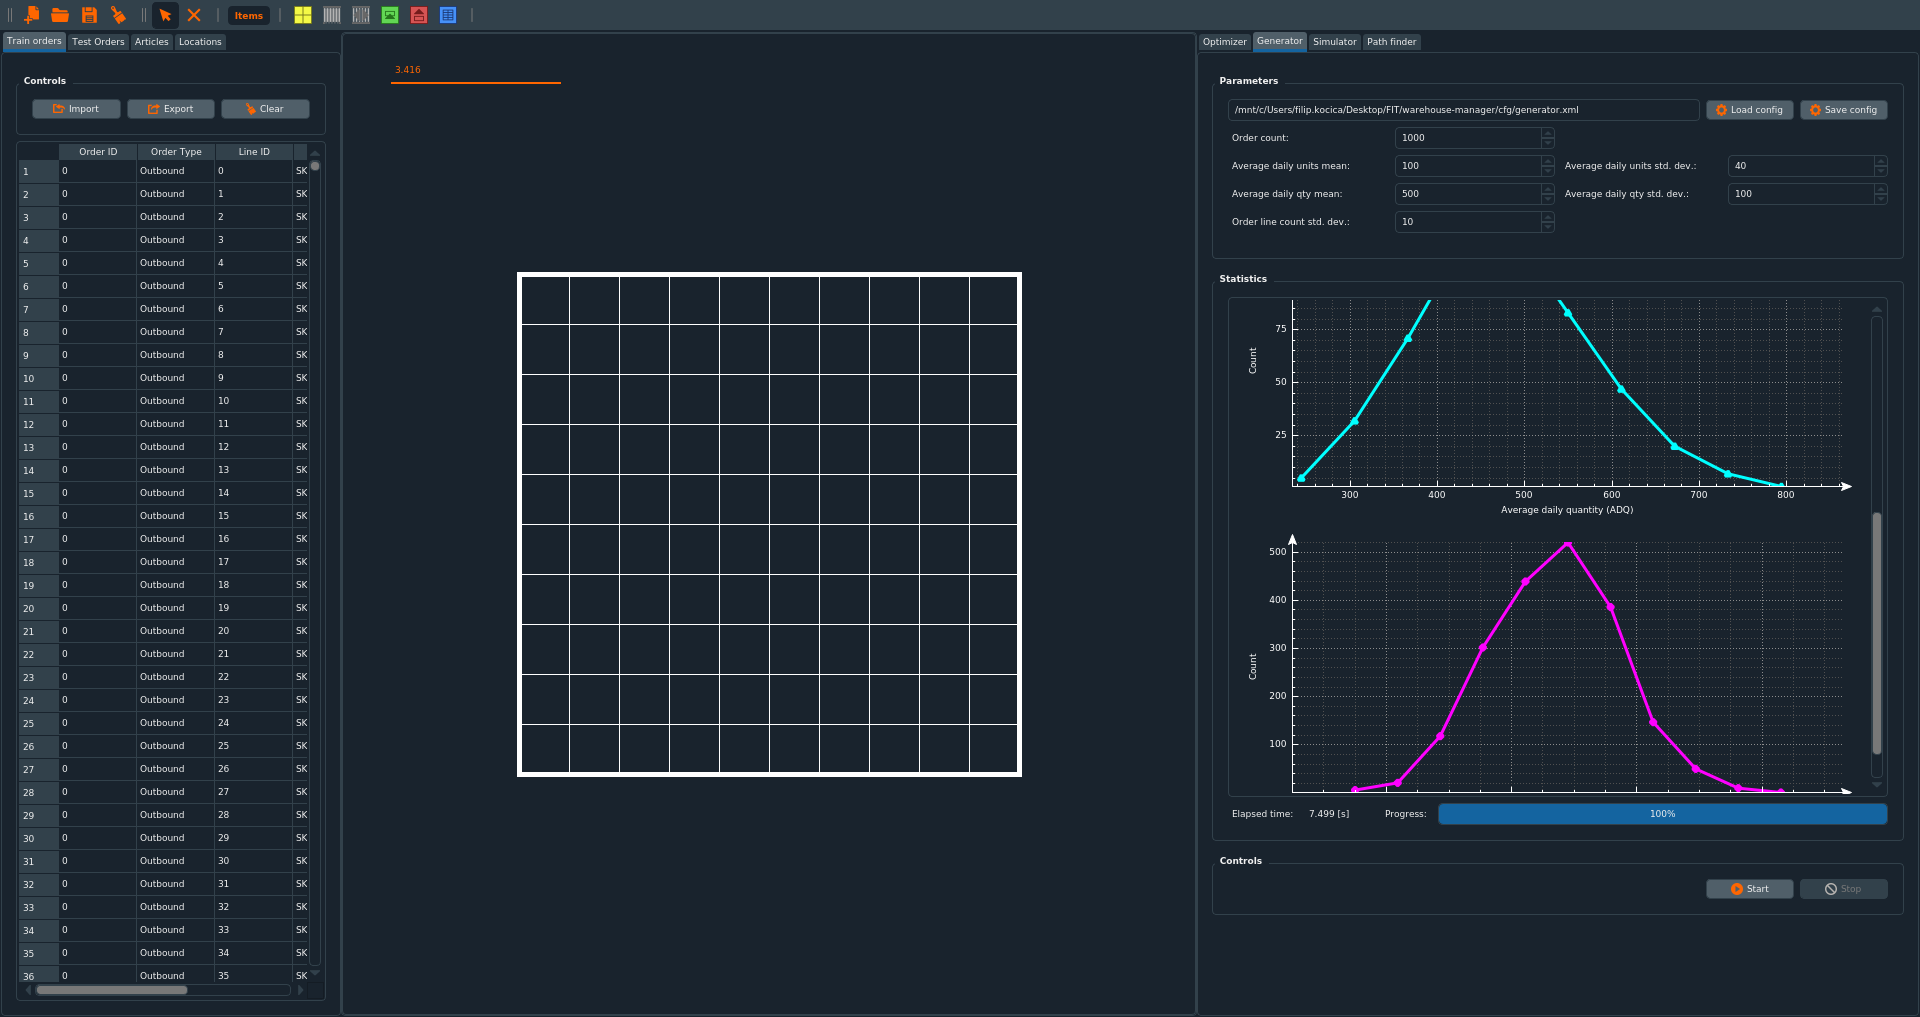
\includegraphics[width=0.99\linewidth]{figures/implementace/WarehouseManagerGen.png}
    \caption{Grafická implementace generátoru objednávek zakomponovaná do aplikace Warehouse Manager. Uprostřed je plocha pro tvorbu modelu skladu. Vpravo je kontrolní panel, kde je možné načíst a nastavit veškeré parametry generování, sledovat tři grafy normálních rozložení (vytvořených z generovaných dat) a spustit či zastavit generování. Vygenerovaná data jsou uložena do panelu s daty vlevo, kde je lze použít pro optimalizátor (první záložka s trénovacími daty), pro simulátor a pathfinder (druhá záložka s testovacími daty), nebo je možné tyto objednávky serializované exportovat do souboru na disk a~opětovně je poté načíst.}
    \label{fig:UI_generator}
\end{figure}

\subsection{Konfigurace}
Generátor objednávek, stejně jako ostatní nástroje, je závislý na vstupu od uživatele, a~proto bylo nutné implementovat způsob zadávání potřebných hodnot. K tomu byly využity konfigurační soubory ve formátu XML. Při použití grafického rozhraní je možné nastavit všechny parametry přímo tam, jak lze vidět na snímku \ref{fig:UI_generator}.

Jednotlivé položky které je uživatel schopen nastavit a jejich významy jsou následující (podrobnější vysvětlení lze najít v sekci \ref{section:impl_gen}):

\begin{itemize}
    \item \texttt{orderCount} -- Počet generovaných objednávek.
    \item \texttt{miAdu} -- Střední hodnota normálního rozložení pro generování ADU produktů.
    \item \texttt{sigmaAdu} -- Rozptyl normálního rozložení pro generování ADU produktů.
    \item \texttt{miAdq} -- Střední hodnota normálního rozložení pro generování ADQ produktů.
    \item \texttt{sigmaAdq} -- Rozptyl normálního rozložení pro generování ADQ produktů.
    \item \texttt{sigmaLines} -- Rozptyl počtu položek objednávek.
\end{itemize}

\subsection{Princip fungování a implementace}
\label{section:impl_gen}
Parametry generovaných sad objednávek, což jsou jejich množství, obsah a velikost, jsou dány uživatelem definovanými pravděpodobnostními rozděleními. Pravděpodobnostní modely, na základě kterých se generování provádí, jsou Gaussova rozložení -- parametry (střední hodnotu a rozptyl) definuje uživatel. Generátor je založen na hodnotách ADU\footnote{\emph{Average daily units} -- průměrný denní počet zakoupení.} a ADQ\footnote{\emph{Average daily quantity} -- průměrná denní zakoupená kvantita.}.

Samotné generování probíhá tak, že se vygeneruje hodnota ADU pro každý produkt $i$~a~spočtou se pravděpodobnosti zakoupení jednotlivých produktů $p_i$ pomocí rovnice:
\begin{equation}
    \label{eq:aduPst}
    p_i = \frac{ADU_i}{\sum_{n=1}^{N} ADU_n},
\end{equation}
z čehož vznikne diskrétní pravděpodobnostní rozložení. Poté se iteruje přes počet objednávek, které chce uživatel vygenerovat. Pro každou takovou objednávku se z normálního rozložení vygeneruje počet položek, které má tato objednávka mít. Poté je pro každou položku nutno vybrat produkt. To se provádí náhodným výběrem z pravděpodobnostního rozložení z rovnice \ref{eq:aduPst}, a tedy čím větší má produkt spočtenou pravděpodobnost zakoupení, tím má vyšší šanci výběru do objednávky. Nakonec se projdou všechny objednávky i jejich položky a pro každou z položek je vygenerována kvantita (zakoupené množství). To se provede tak, že vygenerovaná hodnota z rozložení ADQ pro daný produkt se vydělí počtem zakoupení tohoto produktu, tedy vygenerovaná kvantita se rozdělí mezi zakoupené produkty.

To ve výsledku dává tři Gaussova rozložení, první pro ADU, druhé pro ADQ a třetí pro počet položek objednávky. Vzhledem k tomu, že obě sady objednávek jsou generovány ze stejných pravděpodobnostních rozložení, vzniklé sady jsou různé, avšak spolu korelují.


\section{Simulátor skladu}
Účelem tohoto nástroje je odsimulování zpracování importovaných či generovaných objednávek na vytvořeném modelu skladu tak, jako by to byl reálný skladový systém. Lze jej použít samostatně (např. pro identifikaci úzkých míst, či pro statistickou analýzu), avšak jeho hlavní účel je aproximace kvality nalezeného řešení v optimalizátoru rozložení produktů~--~jinými slovy je použit jako objektivní funkce. Grafickou reprezentaci simulátoru lze vidět na snímku \ref{fig:UI_simulator}.

Autoři práce~\cite{whModelSim} zmiňují, že ze všech možných druhů je nejvhodnější a nejpřirozenější simulace skladu pomocí diskrétních událostí, protože sklad je v podstatě kolekce entit, které reagují na fixní diskrétní události. Simulátor je tedy založen na principu diskrétní simulace a při implementaci byla využita knihovna \texttt{SIMLIB/C++}\footnote{\emph{Simulation Library for \texttt{C++}} -- \url{http://www.fit.vutbr.cz/~peringer/SIMLIB}}. Simulátor poskytuje poměrně komplexní konfiguraci, což umožňuje rozsáhlé možnosti experimentování (od nastavení rychlostí pracovníků a dopravníků až po doplňování produktů, viz \ref{replenishment}).

\subsection{Konfigurace}
Stejně jako předchozí nástroj, je i simulátor konfigurovatelný, a to buď přímo v grafickém rozhraní, nebo \texttt{XML} souborem při použití textového rozhraní. Jednotlivé položky, které je uživatel schopen nastavit a jejich významy jsou následující:

\begin{itemize}
    \item \texttt{toteSpeed} -- Tato hodnota udává, jak rychle jezdí kartony po dopravnících a udává se v metrech za sekundu.
    \item \texttt{workerSpeed} -- Udává rychlost pracovníka, to znamená jak rychle se dokáže pohybovat a vytahovat produkty ze slotů lokací. Opět v metrech za sekundu.
    \item \texttt{totesPerMin} -- Udává, kolik kartonů/objednávek dokáže sklad odeslat za jednu minutu.
    \item \texttt{simSpeedup} -- Umožňuje zrychlení či zpomalení simulace.
    \item \texttt{locationCapacity} -- Udává, kolik objednávek je možné zároveň zpracovávat na jedné lokaci (lze chápat jako počet pracovníků na lokaci).
    \item \texttt{conveyorCapacity} -- Udává, kolik kartonů je možné zároveň převážet pomocí jednoho dopravníku.
    \item \texttt{orderRequestInterval} -- Udává interval, po jehož uplynutí přichází do systému nová objednávka.
    \item \texttt{replenishment} -- Udává, zda má systém počítat s kvantitami produktů a tedy s jejich doplňováním v případě nutnosti.
    \item \texttt{initialSlotQty} -- Tato hodnota říká, jaká je počáteční kvantita produktů v jednotlivých slotech.
    \item \texttt{replenishmentQuantity} -- Udává, kolik produktů se bude doplňovat.
    \item \texttt{replenishmentThreshold} -- Pokud počet produktů ve slotu klesne pod tuto hodnotu, je pro daný produkt spuštěno doplňování produktů.
    \item \texttt{preprocessing} -- Před-zpracování objednávek aby se zrychlila/zjednodušila simulace (tzn. seřazení položek objednávky, aby cesta skladem byla kratší):
    \begin{itemize}
        \item \texttt{None} -- Žádné předzpracování.
        \item \texttt{Normal} -- Předzpracování založené na jednoduchém pravidle porovnávající Manhattanské vzdálenosti jednotlivých lokací. 
        \item \texttt{Optimized} -- Pro každou objednávku je nalezena optimální cesta skladem pomocí nástroje pathfinder, popsaného v sekci \ref{sec:pathFinder}.
    \end{itemize}
\end{itemize}

\begin{figure}[t]
    \centering
    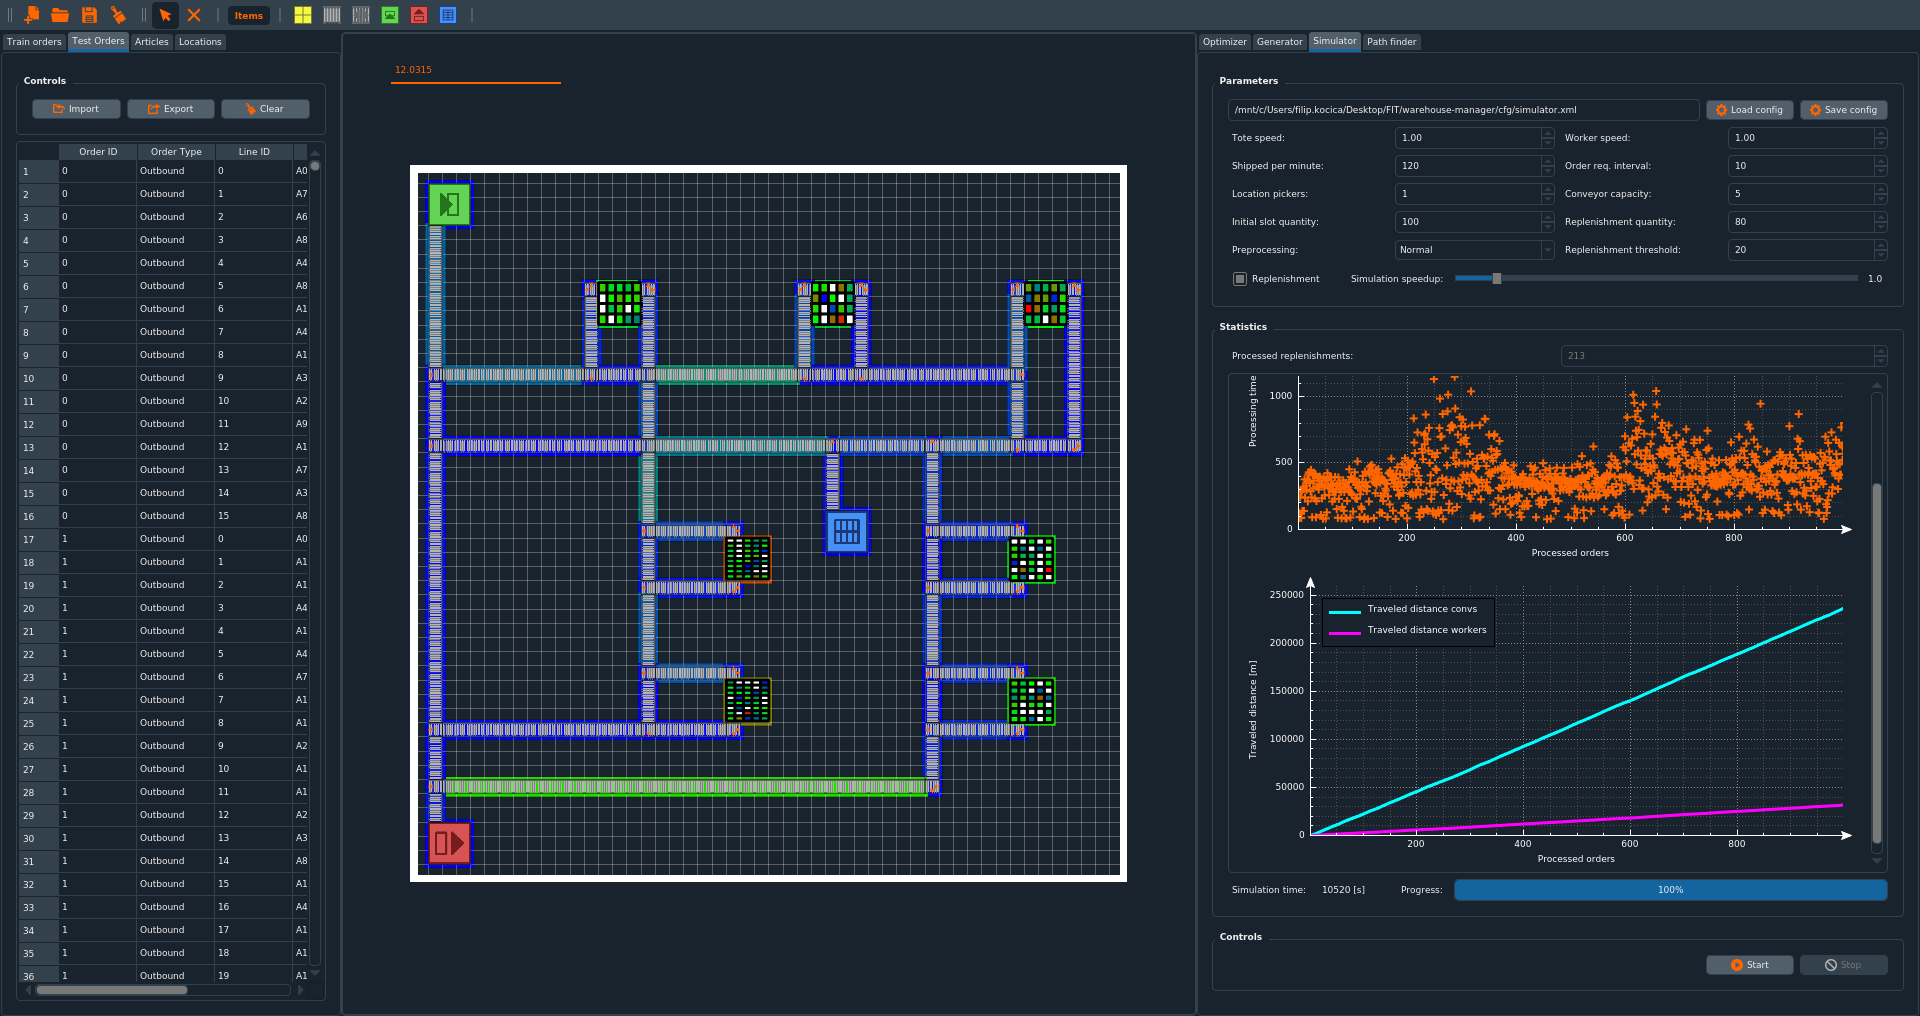
\includegraphics[width=0.99\linewidth]{figures/implementace/WarehouseManagerSim.png}
    \caption{Grafická implementace simulátoru skladu zakomponovaná do aplikace Warehouse Manager. Uprostřed je stále plocha pro tvorbu modelu skladu. Vpravo je kontrolní panel, kde je možné nastavit parametry simulace, sledovat grafy simulace (časy dokončení jednotlivých zákaznických objednávek, nárůst ujeté vzdálenosti na dopravnících a ušlé vzdálenosti pracovníků), vidět počet dokončených doplňovacích objednávek a kontrolovat simulaci (spustit, zastavit). Vlevo jsou data, které simulátor používá, jako je testovací sada objednávek a alokace produktů do slotů lokací. V modelu skladu lze vidět, které sloty lokací jsou zaplněny a je zobrazena také teplotní mapa produktů v lokacích i jednotlivých grafických prvků, kterou lze vidět na snímku~\ref{fig:heatmap} a která reprezentuje zatížení prvků.}
    \label{fig:UI_simulator}
\end{figure}

\subsection{Princip fungování a implementace}
Na začátku se provede načtení objednávek, modelu skladu a alokace produktů do slotů lokací. Poté se provede před-počítání všech možných cest ve skladu, jejich ohodnocení (délka v metrech) a seřazení od nejvýhodnější po nejméně výhodnou. Tímto způsobem lze získat nejvýhodnější cesty mezi všemi prvky/zařízeními ve skladu. Způsob zpracování je popsán pomocí PT sítě na snímku \ref{fig:PTsim}.

%Objednávky jsou modelovány jako diskrétní události (\texttt{class OrderRequest\_t : public simlib3::Event}), které do systému přichází v konfigurovatelných intervalech daných exponenciálním rozložením. Takováto diskrétní událost invokuje zpracování příchozí objednávky pomocí diskrétního procesu \texttt{class OrderProcessor\_t : public simlib3::Process}. Poté se prochází jednotlivé položky objednávky a pro každou z nich se provede vyhledání produktu ve skladu. Po jeho nalezení je nalezena (před-počítaná) optimální cesta a karton se vydává na cestu k cílové lokaci. Přitom projíždí přes jednotlivé dopravníky, které si alokuje pomocí volání knihovny \texttt{SIMLIB}, a sice \texttt{void Enter(Store &s, unsigned long ReqCap=1);}. Výpočet doby, po kterou přes daný dopravník má karton jet se provádí na základě zadaných parametrů, délky dopravníku a velikosti kartonu. Následuje uspání procesu na tuto vypočtenou dobu pomocí volání \texttt{virtual void Wait(double dtime);}. Po probuzení je kapacita opět uvolněna pro následující kartony pomocí volání \texttt{void Leave(Store &s, unsigned long ReqCap=1);}. Tímto způsobem \uv{dojede} karton po jednotlivých dopravnících až k cílové lokaci, ve které se nachází požadovaný produkt. Daný proces si opět alokuje zařízení, v tomto případě lokaci (tzn. další příchozí kartony modelované jako procesy musí čekat, než proces alokující lokaci dokončí práci). Až přijde karton na řadu, tak se opět uspí na vypočtenou dobu, čímž se simuluje pickování pracovníkem skladu nebo robotem. Tato doba je opět dána umístěním produktu v lokaci a nastavenými parametry. Po probuzení a navrácení kapacity se pokračuje další položkou v objednávce a pokračuje se stejným principem. Poté, co jsou všechny položky objednávky zpracovány, karton míří do oblasti odesílání (ang. \emph{shipping area}). Ze zadaných parametrů je vypočtena doba odesílání a je alokována odesílací rampa, proces je uspán a po uplynutí vypočtené doby opět uvolněna kapacita, a tím je objednávka považována za vyřízenou a zahrnuta do statistik. Po zpracování poslední objednávky je uložena nejdůležitější výstupní hodnota, a sice doba která je potřebná ke zpracování všech zadaných objednávek, v daném layoutu skladu a zejména \textbf{s danou alokací produktů do slotů lokací}.

\begin{figure*}[t]
    \centering
    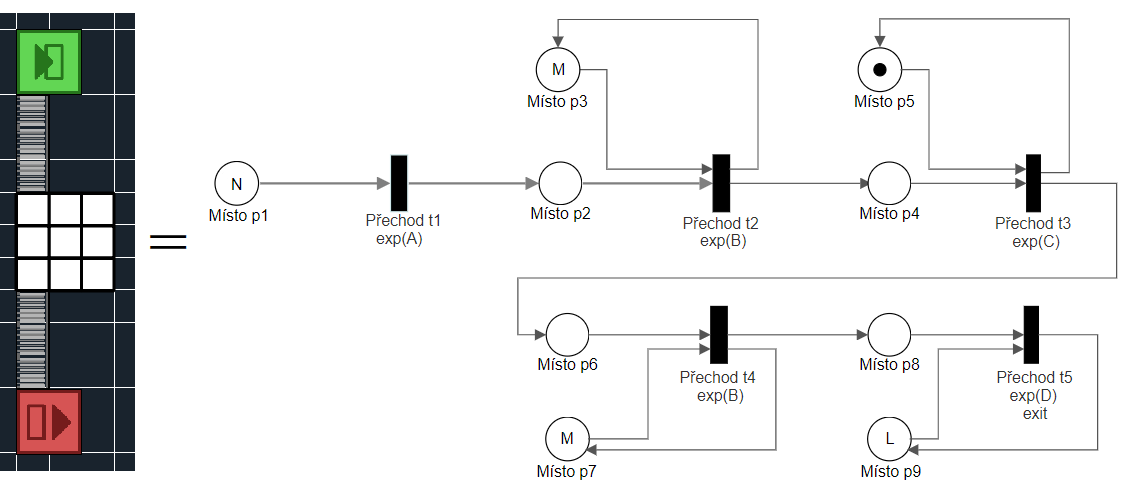
\includegraphics[width=0.71\linewidth]{figures/implementace/PT_wh.png}
    \caption{Triviální sklad se vstupem, jednou lokací a výstupem propojených dopravníkem. Vpravo je odpovídající PT síť. Na začátku se nachází místo \texttt{p1} s \texttt{N} tokeny, kde \texttt{N} se rovná počtu objednávek, které chceme ve skladu zpracovat. Tyto objednávky přichází do systému v časových intervalech (\texttt{A}) daných exponenciálním rozložením. Po vstupu objednávky musí její karton vjet na dopravník. Ten má však omezenou kapacitu danou výpočtem délka dopravníku děleno velikost jednoho kartonu (\texttt{M}). Doba po kterou jede karton po dopravníku je vypočtena jako poměr délky dopravníku a rychlosti kartonu (\texttt{B}). Poté karton vjede do lokace, kde si alokuje pickera na dobu (\texttt{C}), která je spočtena jako suma doby pickování všech produktů, které se v této lokaci mají pickovat. Obdobně karton projede další dopravník a nakonec je karton odeslán ze skladu -- je spočtena doba odesílání jedné objednávky (\texttt{D}), a také kolik jich lze odesílat zároveň (\texttt{L}). Vesměs všechny hodnoty v celém procesu jsou konfigurovatelné.}
    \label{fig:PTsim}
\end{figure*}

\subsection{Paralelní simulace}
\label{section:sim_multithreaded}
Simulátor je využíván mj. optimalizačním nástrojem pro vyhodnocení kvality řešení. Taková simulace je spouštěna pro každého jedince populace v každém kroku evolučního algoritmu. To v případě velkých populací vede k velmi dlouhému trvání optimalizace. Vzhledem k~tomu, že knihovna \texttt{SIMLIB/C++} nebyla koncepčně navržena pro účely paralelního zpracování, nebylo možné provést zrychlení použitím více vláken.

\begin{figure*}[t]
    \centering
    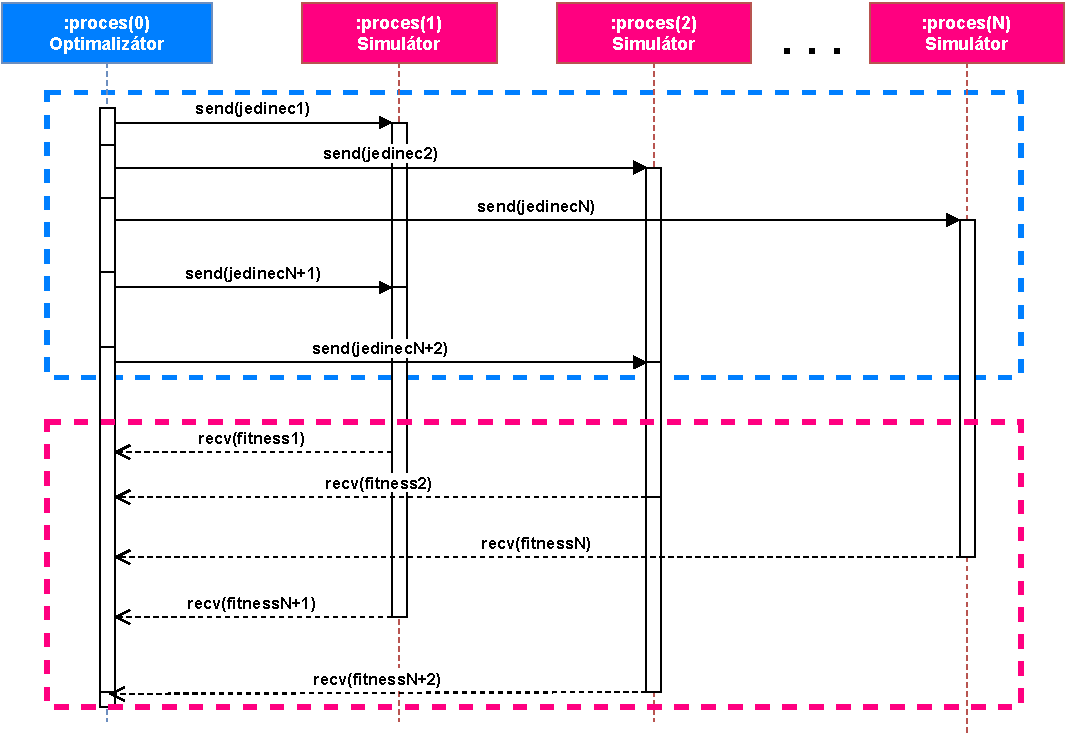
\includegraphics[width=0.8\linewidth]{figures/implementace/SimulationMessageSequence.pdf}
    \caption{Sekvenční diagram znázorňující paralelizaci optimalizace (rovnoměrné rozdělení výpočtu simulací všech jedinců populace mezi $N$ procesů). Modrý obdélník označuje odeslání jedinců na simulaci a růžový pak vysbírání výsledků doby simulace od jednotlivých potomků.}
    \label{fig:simulationMsgSeq}
\end{figure*}

Tento problém byl vyřešen spuštěním několika instancí (procesů) využívající tuto knihovnu, které se nijak neovlivňují a mohou fungovat souběžně. Před začátkem optimalizace je tedy vytvořeno $N$ (konfigurovatelné) takových procesů. Účel takto vytvořených potomků je jednoduchý, a sice provést inicializaci (objednávek, modelu skladu a před-počítání cest), očekávat data, provést simulaci a vrátit výsledek simulace hlavnímu procesu. Po odeslání dat zpět rodiči potomek opět vstupuje do blokujícího čekání na data nebo ukončení komunikace a tedy i samotného potomka. Komunikace mezi rodičem a potomky je znázorněna na snímku~\ref{fig:simulationMsgSeq}.

\begin{itemize}
    \item Od rodiče k potomkům se posílá zakódovaná alokace produktů do jednotlivých slotů (celočíselné pole).
    \item Od potomků zpět k rodiči se posílá výsledek (doba) simulace, a sice hodnota \emph{fitness} (číslo s plovoucí řádovou čárkou).
\end{itemize}

Jedinci (potažmo jejich simulace) jsou mezi procesy rozděleny zcela rovnoměrně a zrychlení optimalizace pomocí paralelizace simulací bylo velmi značné.



\subsection{Řešení problému duplicitních jedinců}
\label{section:sim_duplicit_jedinci}
Dále bylo zjištěno, že až $30\%$ všech jedinců v populaci je duplicitních (stejných jako nějaký jiný jedinec). Byl proto implementován mechanismus převodu zakódovaných genů jedince na řetězec, a pomocí hashovací tabulky bylo zajištěno, že se nebudou provádět duplicitní simulace, ale jedinci se stejnými geny si pouze překopírují již spočtený výsledek jiného jedince. To vedlo k ještě většímu zrychlení celého procesu a optimalizace i opravdu komplexního skladu bylo možné počítat v řádu maximálně několika dní.

\subsection{Doplňování produktů}
\label{replenishment}
%Doplňování produktů (ang. \emph{replenishment}) je proces, při kterém se ze zásobníku produktů (označován jako \emph{buffer}) doplňují produkty do slotů lokací, ze kterých se následně pickují zákaznické objednávky. Toto se typicky provádí ve chvíli, kdy množství produktů ve slotu klesne pod určitou úroveň (konfigurovatelná v XML/UI). Tento mechanismus byl implementován za účelem zvýšení realističnosti simulace skladu.

%Implementace doplňování produktů je následující: do konfigurátoru skladu byl přidán nový grafický prvek, zásobník produktů, ze kterého se budou produkty doplňovat do lokací a uživatel si jej může umístit kam chce (a připojit dopravníkem ke zbytku skladu). Následně byl přidán nový typ objednávky, a tedy se v systému mohou vyskytovat dva typy objednávek:

%\begin{enumerate}
%    \item \emph{Outbound} -- odchozí zákaznická objednávka.
%    \item \emph{Replenishment} -- interní objednávka určená pro doplňování produktů.
%\end{enumerate}

%Objednávka pro doplňování je v podstatě úplně stejná jako odchozí zákaznická objednávka, liší se pouze typem. Je tedy také zpracovávána pomocí diskrétního procesu \texttt{class OrderProcessor\_t : public simlib3::Process}. V případě, že v některé z lokací klesne množství produktů ve slotu pod konfigurovanou úroveň, je vytvořena objednávka pro doplňování a jsou ji přidány položky se všemi produkty, které jsou v dané lokaci a jejich kvantita je pod danou úrovní. Kvantita položek je nastavena na předem konfigurovanou hodnotu. Tato objednávka je stejně jako odchozí objednávka reprezentována jako proces v systému a po cestě ze zásobníku k lokaci se chová úplně stejně. Poté, co se objednávka pro doplnění dostane do cílové lokace, jsou veškeré produkty z objednávky doplněny do slotů lokace, kam patří (což pracovníkovi opět zabere jistý čas podle pozice slotu).

%\paragraph{Objednávky, které nelze napickovat} Může se stát, že množství produktů ve slotu klesne pod kvantitu, kterou vyžaduje některá z odchozích objednávek. Takovou objednávku nelze v daný moment dokončit a proces dané objednávky je deaktivován a musí čekat na doplňovací objednávku, což lze v systému chápat jako penalizaci. Poté, co přijde objednávka pro doplnění produktů a je dokončena, jsou všechny takto deaktivované procesy reprezentující odchozí objednávky (na dané lokaci) opět aktivovány. Každá z takto aktivovaných objednávek zkontroluje, zda už ji lze napickovat (na cestě může být více objednávek pro doplnění). Pokud ji nelze napickovat, proces se opět deaktivuje a čeká na \uv{svou} doplňovací objednávku. V opačném případě se provede pickování a objednávka pokračuje ve své cestě skladem.

Doplňování produktů (ang. \emph{replenishment}) je proces, při kterém se ze zásobníku produktů doplňují produkty do slotů, ze kterých se pickují zákaznické objednávky. Toto se typicky provádí ve chvíli, kdy množství produktů ve slotu klesne pod určitou (konfigurovatelnou) úroveň. Tento mechanismus byl implementován za účelem zvýšení realističnosti simulace skladu.

Objednávka pro doplňování je v podstatě úplně stejná jako zákaznická objednávka a~je také reprezentována jako proces v systému, a také se tak chová. Poté, co se objednávka pro doplnění dostane do cílové lokace, jsou veškeré produkty z objednávky doplněny do příslušných slotů lokace a objednávka je ukončena.

Zákaznické objednávky, které nelze napickovat z důvodu nedostatku produktů ve slotu jsou deaktivovány a musí čekat na doplňovací objednávku, což lze v systému chápat jako penalizaci. Poté, co přijde objednávka pro doplnění produktů a je dokončena, jsou všechny takto deaktivované procesy reprezentující zákaznické objednávky (na dané lokaci) opět aktivovány a zkontrolují, zda už je lze napickovat nebo se musí znovu uspat a čekat na \uv{svou} doplňovací objednávku.



\section{Pathfinder}
\label{sec:pathFinder}
Nástroj pro optimalizaci cesty byl implementován skrze evoluční algoritmus $\mathcal{MAX}\!{-}\!\mathcal{MIN}$ mravenčí systém, a nazývá se pathfinder. Cílem tohoto nástroje je nalézt optimální cestu objednávky skrze sklad, tak, aby urazila co nejkratší možnou vzdálenost. Vzhledem k tomu, že každá objednávka potřebuje navštívit jiné lokace, optimální cesta skrze sklad se zpravidla liší, a proto je nutné optimální cestu hledat pro každou objednávku samostatně. Grafická nástavba dokáže mimo tvorbu grafu také zvýraznit aktuálně nejlepší nalezenou cestu vybrané objednávky skrze sklad a očíslovat grafické prvky, aby bylo zřejmé, v jakém pořadí je objednávka navštíví. Implementace je inspirována \texttt{MAX-MIN-Ant-System}\footnote{\url{https://github.com/RSkinderowicz/MAX-MIN-Ant-System}}.

\subsection{Konfigurace}
Hledač cest je konfigurovatelný buď pomocí konfiguračního souboru ve formátu \texttt{XML}, či v~grafickém rozhraní a význam jednotlivých položek je následující:

\begin{itemize}
    \item \texttt{antCount} -- Počet umělých mravenců v kolonii.
    \item \texttt{rho} -- Udává míru vypařování feromonů.
    \item \texttt{beta} -- Hodnota použitá pro výpočet matice heuristik.
    \item \texttt{probBest} -- Pravděpodobnost, že výsledně řešení bude obsahovat pouze nejlepší hrany.
    \item \texttt{nearestNeighbours} -- Počet nejbližších sousedů uložených pro každý uzel.
    \item \texttt{probUseIterationBest} -- Pravděpodobnost s jakou bude pro aktualizaci feromonů použit nejlepší dosažený výsledek v dané iteraci. S pravděpodobností rovnou doplňku této hodnoty do jedné bude pro aktualizaci použit dosavadní nejlepší výsledek.
    \item \texttt{maxIterations} -- Maximální počet iterací mravenčího algoritmu.
    \item \texttt{selectedOrderID} -- Jednoznačný identifikátor objednávky, pro kterou se má optimální cesta počítat.
\end{itemize}

\begin{figure}[t]
    \centering
    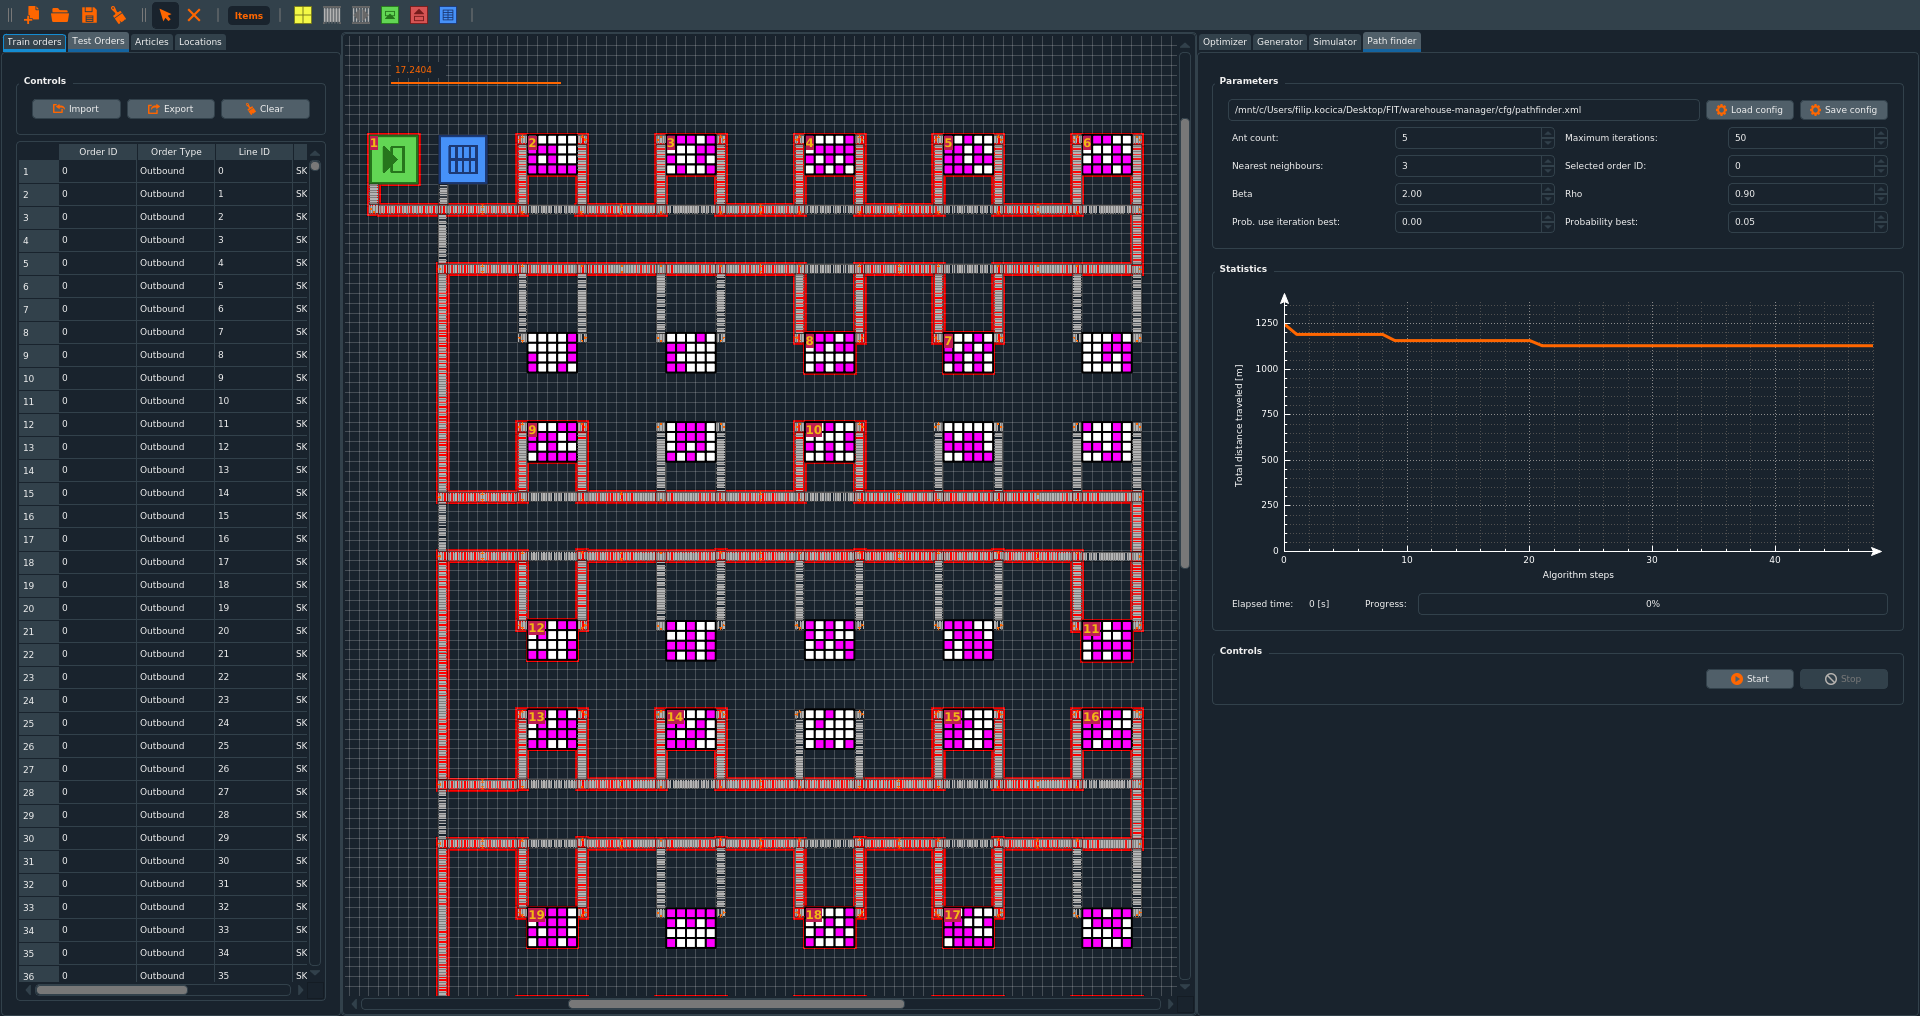
\includegraphics[width=0.99\linewidth]{figures/implementace/WarehouseManagerPaf.png}
    \caption{Grafická implementace nástroje pathfinder zakomponovaná do aplikace Warehouse Manager. Uprostřed je stále plocha pro tvorbu modelu skladu. Vpravo je kontrolní panel, kde je možné nastavit parametry nástroje, sledovat graf objektivní funkce a spustit či zastavit hledání optimální cesty. Vlevo jsou opět data používaná nástrojem (objednávky, produkty a sloty lokací). Nástroj je v grafickém rozhraní implementován v separátním vlákně, aby neblokoval hlavní okno. Po každém kroku optimalizačního algoritmu se však provádí zpětné volání (ang. \emph{callback}) do hlavního vlákna pro přidání nové hodnoty do grafu objektivní funkce a překreslení aktuální nejkratší cesty. Cesta je červeně zvýrazněna a prvky skladu jsou doplněny o čísla aby bylo jasné pořadí, v jakém je bude objednávka navštěvovat.}
    \label{fig:UI_pathFinder}
\end{figure}

\subsection{Princip fungování a implementace}
Na začátku výpočtu se nalezne vstup do skladu (který bude použit vždy jako počátek cesty mravence) a výstup ze skladu (který bude použit vždy jako poslední prvek cesty mravence). Následně se z položek vybrané objednávky zjistí, které lokace musí tato objednávka navštívit (ty budou součástí cesty mezi zmíněným počátkem a koncem). Toto vytvoří graf, který je potřeba projít.

Následně probíhá inicializace matice vzdáleností jednotlivých uzlů (prvků skladu), matice heuristik a nakonec nalezení N (konfigurovatelné) nejbližších sousedů pro každý uzel. Vzdálenost mezi jednotlivými uzly není Eulerova (\uv{vzdušnost čarou}), nýbrž Manhattanská, respektující délku pravoúhle propojených dopravníků propojující tyto dva uzly.

Pro výpočet počátečních limitů hodnot feromonů je nutné sestavit počáteční řešení problému tzv. \uv{hltavým} způsobem, tzn. první jsou do řešení přidáni všichni nejbližší sousedi daného uzlu, a poté zbytek všech uzlů. Poté lze inicializovat matici udávající množství feromonů na přechodech mezi jednotlivými uzly -- kde jsou všechny přechody inicializovány na maximální hodnotu feromonu.

Poté je zahájen výpočet, kdy se v každé iteraci algoritmu sestaví N řešení (mravenců reprezentujících cestu, konfigurovatelné), kterým je následně spočtena délka cesty. Poté je nalezeno nejlepší řešení v dané iteraci a pokud je třeba, tak i aktualizováno dosavadní nejlepší nalezené řešení. Poté je množství feromonu sníženo o míru vypařování a hranám, přes které prochází nejlepší řešení je doplněn feromon v závislosti na kvalitě daného řešení.

Po dosažení před-definovaného množství iterací se vypíše nejlepší nalezený výsledek. V~případě, že je zapnuta i grafická nástavba, jsou průběžné výsledky pomocí zpětného volání posílány do grafického rozhraní (aby se pro každou iteraci mohlo vykreslit nejlepší nalezené řešení) a souběžně je tvořen graf udávající nejkratší délku cesty v každé iteraci, jak lze vidět na snímku \ref{fig:UI_pathFinder}. Tento nástroj je možné použít pro nalezení optimální cesty každé objednávky v simulátoru.

\section{Optimalizátor rozložení produktů}
Automatizované sklady jsou mnohdy velmi komplexní systémy a mají mnohá omezení daná jejich layoutem, způsobem manipulace s produkty, úložnými a pickovacími politikami atd. Optimalizace výkonnosti takovýchto skladů často vyžaduje přesnou definici jejich modelu a nelze jej jednoduše převést na matematický výraz. Vzhledem k tomu, a také k možnosti uživatele si vlastnoručně vytvořit model skladu, by bylo velmi obtížné takto obecně vytvořit matematický popis skladu, proto tato práce pro vyhodnocení kvality používá simulaci, která odpovídá reálnému fungování skladu. Hlavní myšlenka optimalizátoru v této práci je minimalizace doby nutné pro zpracování všech objednávek skrze vhodné rozložení produktů do jednotlivých slotů v lokacích skladu. Doba zpracování objednávek je aproximována simulátorem popsaném v předešlé kapitole. Doba zde představuje simulační čas, nikoli reálný. Grafickou implementaci lze vidět na snímku~\ref{fig:UI_optimalizator}.

Pro nalezení optimální distribuce produktů do slotů lokací byl jako nejvhodnější přístup vybrán GA (genetický algoritmus), a to protože nepotřebuje znát matematický popis problému, pouze problém zakódovat jako sekvenci čísel. Dále byly však pro porovnání implementovány další tři evoluční algoritmy, a sice: DE (diferenční evoluce), ABC (algoritmus umělých včelstev) a PSO (optimalizace rojem částic). Všechny tyto algoritmy pracují standardně ve spojitém prostoru, a tedy bylo potřeba je na základě odborných prací~\cite{ABC_TSP, DE_GA_TSP, PSO_GA_TSP, orderedCrossover, GA_TSP} redefinovat pro diskrétní prostor. K tomu pomohla zejména velká podobnost problematiky SLAP a TSP (problému obchodního cestujícího), pro který byly tyto redefinice v odborných článcích popsány).

\begin{figure}[t]
    \centering
    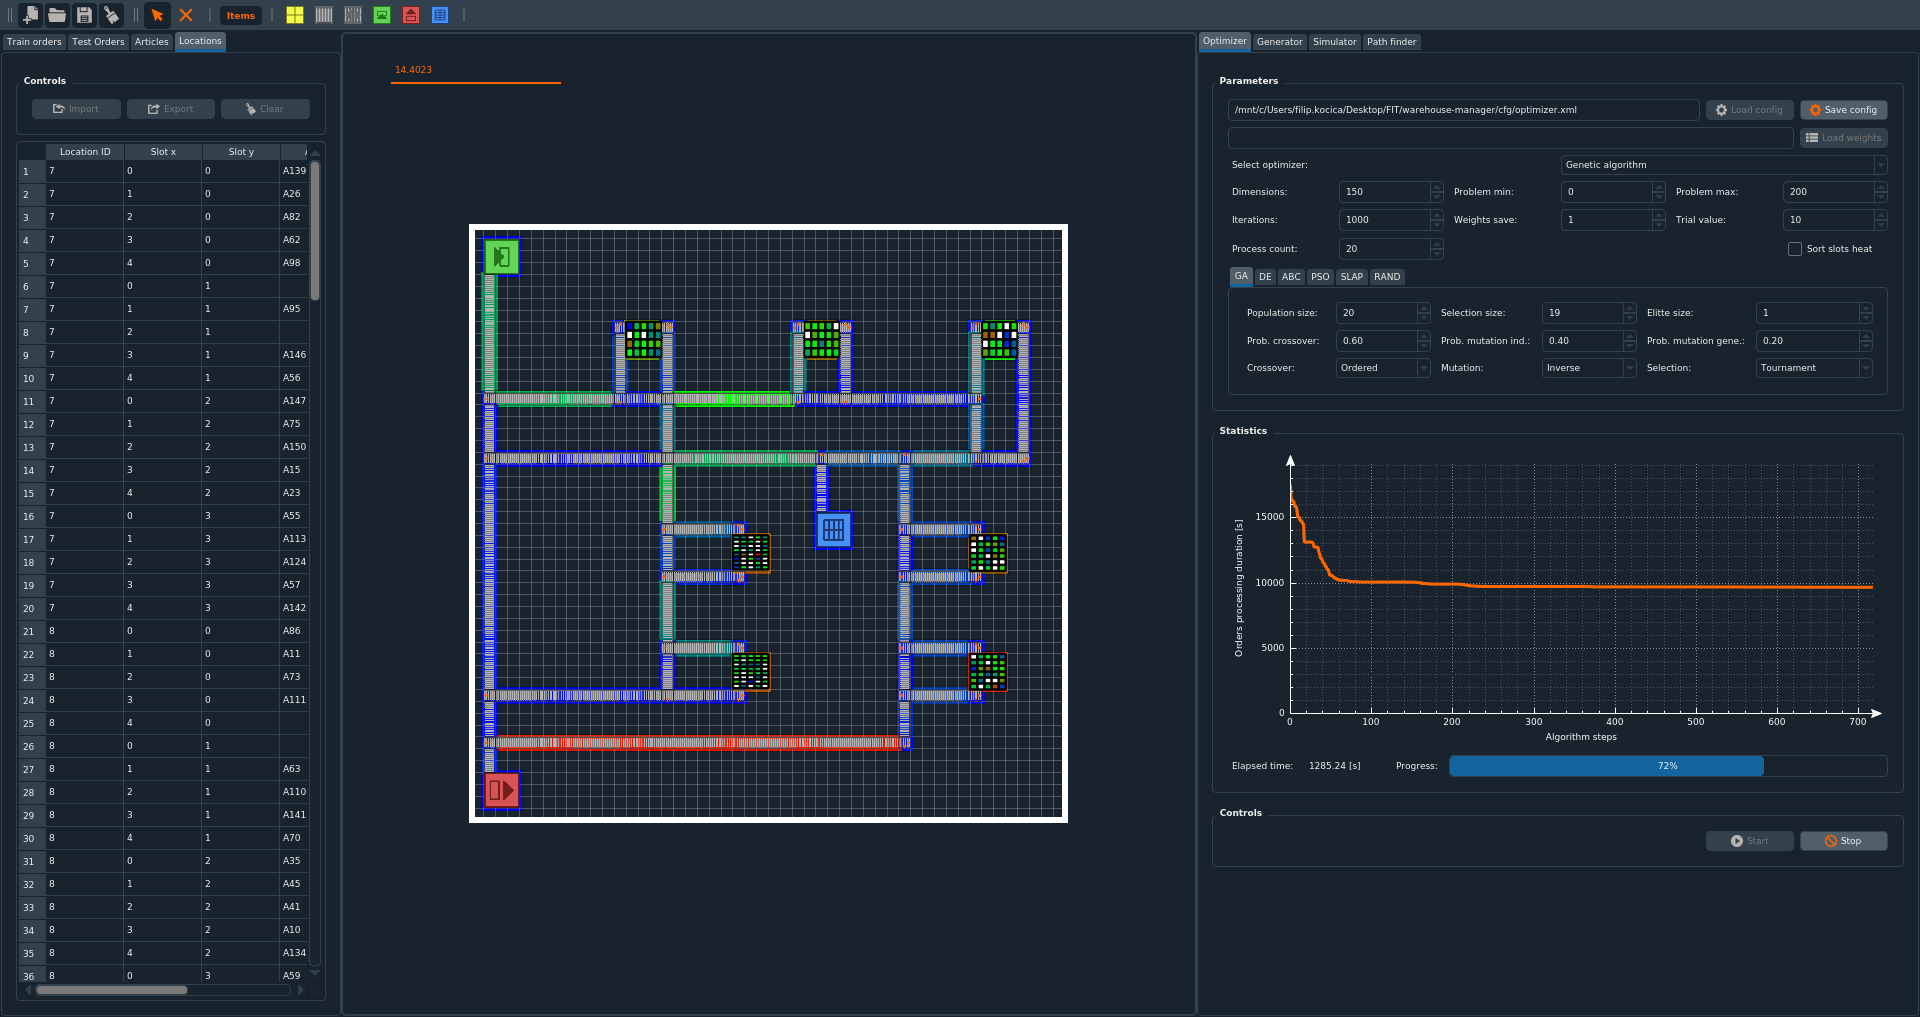
\includegraphics[width=0.99\linewidth]{figures/implementace/WarehouseManagerOpt.png}
    \caption{Grafická implementace optimalizátoru skladu zakomponovaná do aplikace Warehouse Manager. Uprostřed je stále plocha pro tvorbu modelu skladu. Vpravo je kontrolní panel, kde je možné nastavit parametry optimalizace (a vybrat si optimalizační algoritmus a do-nastavit jej v příslušné záložce), vidět graf objektivní funkce a spustit či zastavit optimalizaci. Vlevo jsou opět data používaná optimalizátorem (trénovací objednávky, produkty a sloty lokací). Optimalizátor je v grafickém rozhraní implementován v separátním vlákně, aby neblokoval hlavní okno. Po každém kroku optimalizačního algoritmu se provádí zpětné volání do hlavního vlákna pro přidání nové hodnoty do grafu a překreslení aktuální alokace produktů ve slotech a aktuálního zatížení prvků.}
    \label{fig:UI_optimalizator}
\end{figure}

\subsection{Kódování}
Pro použití evolučních algoritmů bylo nutné navrhnout vhodný způsob kódování řešení. Každý ze čtyř použitých evolučních algoritmů (genetické algoritmy, diferenční evoluce, algoritmus umělých včelstev i optimalizace rojem částic) používají jiné názvosloví. Např. v~genetických algoritmech se pro jedno zakódované řešení problému používá výraz jedinec či chromozom. V algoritmu umělých včelstev je to pak včela či zdroj potravy a v optimalizaci rojem částic je to částice či jedinec. Vzhledem k tomu, že pojem \uv{jedinec} se vyskytuje nejčastěji a nejlépe vystihuje podstatu, bude v tomto textu řešení problému označováno jako jedinec.

\begin{figure}[t]
    \centering
    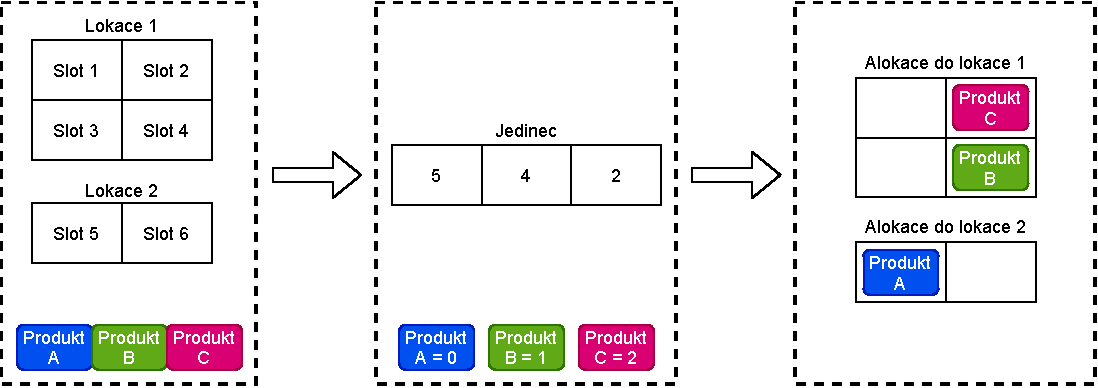
\includegraphics[width=0.99\linewidth]{figures/implementace/ChromosomeEncoding.pdf}
    \caption{Triviální příklad pro navržené kódování. Mějme dvě lokace, první se čtyřmi sloty, druhou se dvěma sloty. Do těchto lokací chceme alokovat tři produkty: A, B, C. Každému slotu je přiřazen unikátní celo-číselný identifikátor. Vezmeme v potaz jednoho jedince populace, který má délku stejnou jako je počet produktů, což je tři. První index reprezentuje první produkt, druhý index druhý produkt atd. Čísla na jednotlivých indexech reprezentují slot, do kterého je produkt alokován. Tzn. produkt A, který obsahuje hodnotu $5$ bude umístěn do slotu $5$, který se nachází v druhé lokaci.}
    \label{fig:chromosomeEncoding}
\end{figure}

Výhodou je, že všechny čtyři algoritmy používají stejné kódování jedinců, proto mohla být vytvořena bázová třída se všemi společnými operacemi (jako inicializace populace, provedení simulace všech jedinců, apod.). Všechny algoritmy byli implementovány ve vlastní třídě vždy odvozené z bázové třídy, což mimo jiné umožnilo využití polymorfismu. Vzhledem k podstatě problému, který byl řešený v diskrétním prostoru, byl zakódovaný jedinec reprezentován jednoduše jako vektor celých čísel. Tento vektor má vždy délku stejnou jako je počet produktů, které se algoritmus snaží optimálně rozdistribuovat do slotů lokací. Jednotlivé položky (zvané jako geny, \emph{allele} hodnoty, apod.) poté nabývají celých čísel reprezentující slot lokace, do kterého bude daný produkt uložen. Všem slotům, které se ve skladu nachází algoritmus přiřadí unikátní celočíselný identifikátor, který se poté používá jako hodnota ve vektoru každého jedince). Příklad znázorňující toto kódování lze najít na obrázku \ref{fig:chromosomeEncoding}.

Tento přístup má však také svá omezení:

\begin{enumerate}
    \item Počet produktů může být rozdílný od počtu slotů lokací, avšak počet slotů musí být vyšší než nebo stejný jako je počet produktů (aby byl každý produkt někam umístěn).
    \item Pokud by bylo provedeno klasické křížení či mutace jedinců bez omezujících podmínek, s velkou pravděpodobností by v jedinci vznikly duplikáty celočíselných hodnot, což by značilo, že více produktů je umístěno do stejného slotu, což není možné.
    \item Bod dva by také implikoval, že některé produkty by nebyly přiřazeny do žádného slotu, což by způsobilo, že objednávky s těmito produkty by nebylo možné dokončit.
\end{enumerate}

Vyjma prvního bodu jsou tyto omezující podmínky v podstatě principiálně stejné, jako tomu je u problému obchodního cestujícího. V podkapitole \ref{section:redefiniceTSP} byla popsána teorie redefinice jednotlivých evolučních algoritmů pro diskrétní prostor a pro řešení problematiky obchodního cestujícího. Tato redefinice byla provedena pro čtyři zmíněné evoluční algoritmy.

\subsection{Grafická teplotní mapa}
Jak lze vidět na snímku \ref{fig:UI_optimalizator}, každý ze zaplněných slotů produktem má jinou barvu. To značí, jak velké má produkt ADU -- tzn. interpretace množství zakoupení produktu pomocí teplotní mapy (ang. \emph{heatmap}). Vzhledem k tomu, že jednotlivé zařízení ve skladu (dopravníky, lokace, ...) mohou mít různé zatížení (t.j. doba, po kterou je zařízení v provozu z~pohledu doby celé simulace), byl implementován mechanismus na zjištění zatížení jednotlivých prvků a jeho grafického znázornění. Grafická vizualizace využívá teplotní mapu na obrázku \ref{fig:heatmap}, a to tak, že kolem jednotlivých prvků vytvoří barevné ohraničení. A tedy nejvíce vytížené prvky budou mít ohraničení rudě červené, zatímco téměř nevyužité prvky tmavě modré. Tento mechanismus by měl uživatelům pomoct identifikovat \uv{úzká místa} ve skladu. Uživatelé pak mohou zkusit přijít na řešení pomocí distribuce zátěže mezi více zařízení a opětovné simulace, nebo nechat optimalizátor se s tímto problémem vypořádat za ně. Přidáním přídavných dopravníků se značně snížila zátěž a průchod skladem se zrychlil. Toto zatížení se v případě textového použití optimalizátoru či simulátoru vypisuje textově.

\addtocounter{footnote}{-1}

\begin{figure}[t]
    \centering
    
\includegraphics[width=0.5\linewidth]{figures/implementace/heatmapOptimizer.png}
    \caption{Grafická vizualizace použité teplotní mapy. Čím jsou produkty častěji kupované (vyšší ADU), tím je barva slotu do kterého jsou umístěny více vpravo (tzn. nejčastěji kupovaný produkt bude reprezentován červeně). Stejná teplotní mapa je použita také pro reprezentaci zatížení skladových prvků jako jsou dopravníky a lokace\protect\footnotemark{}.}
    \label{fig:heatmap}
\end{figure}


\subsection{Konfigurace}
Nástroj lze opět konfigurovat pomocí \texttt{XML} souboru či v grafickém rozhraní a jednotlivé položky které je uživatel schopen nastavit a jejich významy jsou následující -- první blok jsou obecné parametry použité ve více algoritmech, následuje blok s parametry pro genetické algoritmy a zbytek byl pro úsporu místem vynechán:

\begin{itemize}
    \item \texttt{numberDimensions} -- Rozměr problému, neboli velikost jedince.
    \item \texttt{problemMin} -- Nejnižší hodnota, které může gen nabývat.
    \item \texttt{problemMax} -- Nejvyšší hodnota, které může gen nabývat.
    \item \texttt{maxIterations} -- Maximální počet cyklů optimalizačního algoritmu.
    \item \texttt{initialWeights} -- Počáteční váhy (alokace produktů do slotů).
    \item \texttt{saveWeightsPeriod} -- Po kolika cyklech algoritmu se má ukládat nejlepší řešení.
    \item \texttt{maxTrialValue} -- Maximální počet cyklů bez zlepšení fitness, než bude jedinec vyhozen z populace.
    \item \texttt{procCount} -- Počet procesů, které se mají vytvořit pro účely simulace jedinců.
    \item \texttt{slotHeatReorder} -- Produkty v každé z lokací jsou před každým optimalizačním krokem seřazeny podle toho, jak často jsou kupovány.
    \item \texttt{populationSize} -- Velikost populace pro genetické algoritmy.
    \item \texttt{selectionSize} -- Velikost vybrané části pro křížení pro genetické algoritmy.
    \item \texttt{eliteSize} -- Velikost elite (neměnné) části pro genetické algoritmy.
    \item \texttt{probCrossover} -- Pravděpodobnost křížení dvou jedinců.
    \item \texttt{probMutationInd} -- Pravděpodobnost mutace jedince.
    \item \texttt{probMutationGene} -- Pravděpodobnost mutace genu.
    \item \texttt{mutationFunctor} -- Funkce, která se má použít pro mutaci jedince (\texttt{mutateOrdered}, \texttt{mutateInverse}).
    \item \texttt{selectionFunctor} -- Funkce, která se má použít pro selekci jedinců (\texttt{selectRank}, \texttt{selectTrunc}, \texttt{selectTournam}, \texttt{selectRoulette}).
    \item \texttt{crossoverFunctor} -- Funkce, která se má použít pro křížení jedinců (\texttt{crossoverOrdered}, \texttt{crossoverHeuristic}, \texttt{crossoverBinomical}).
    \item A mnoho dalších parametrů pro ABC, DE, PSO, SLAP a náhodné prohledávání\ldots
    %\item \texttt{foodSize} -- Velikost populace (resp. počet včel či zdrojů jídla) algoritmu umělých včelstev.
    %\item \texttt{keepBest} -- Pokud je nastaveno na \uv{pravda}, nejlepší výsledek se nezahazuje (\texttt{trial}).
    %\item \texttt{numberParticles} -- Velikost populace (resp. počet částic) algoritmu optimalizace rojem částic.
    %\item \texttt{correctionFactor1} --  Faktor učení osobní změny.
    %\item \texttt{correctionFactor2} -- Faktor učení sociální změny
    %\item \texttt{weighing} -- Hodnota \emph{inertia}.
    %\item \texttt{crossoverFunctorPSO} -- Funkce, která se má použít pro křížení jedinců (\texttt{crossoverOrdered} viz \ref{fig:orderedCrossover}, \texttt{crossoverHeuristic} viz algoritmus \ref{alg:diskretniPSO}).
    %\item \texttt{populationSizeDE} -- Velikost populace algoritmu diferenční evoluce.
    %\item \texttt{scalingFactor} -- Faktor škálování (reálné číslo, které slouží pro kontrolu rychlosti evoluce).
    %\item \texttt{probCrossoverDE} -- Pravděpodobnost provedení křížení.
    %\item \texttt{crossoverFunctorDE} -- Funkce, která se má použít pro křížení jedinců (\texttt{crossoverOrdered} \ref{fig:orderedCrossover}, \texttt{crossoverBinomical} viz \ref{binomicalCrossover}).
    %\item \texttt{balanceTheLoad} -- Parametr pro SLAP, který pokud je aktivní, tak rozděluje produkty rovnoměrně mezi všechny lokace.
    %\item \texttt{populationSizeRand} -- Velikost \uv{populace} pro náhodné prohledávání.
\end{itemize}

\footnotetext{Obrázek převzat~z~\url{https://stackoverflow.com/a/20793850/8254699}.}


\subsection{Experimenty}
Optimalizace skladu pomocí genetického algoritmu jako taková přinášela velmi dobré výsledky. Avšak stále se nabízely nové způsoby, jak dosáhnout lepších výsledků nebo alespoň podnětného porovnání.

\paragraph{Optimalizátory pro porovnání}
Mimo čtyři optimalizátory rozložení produktů založené na evolučních algoritmech, byly implementovány také dva \uv{optimalizátory} určené čistě pro účely porovnání. První z nich je náhodné prohledávání. Dalším je optimalizátor založený na klasickém přístupu k rozřazení produktů ve skladu převzatý z práce~\cite{slapSeacomp}. Je založený na principu spočtení vzdálenosti každého slotu od vstupního a výstupního bodu skladu, a~jejich seřazení. Dále spočtení, jak často jsou kupovány jednotlivé produkty a jejich seřazení. Následně jsou tyto seřazené produkty namapovány na seřazené sloty lokaci (nejčastěji kupovaný produkt do nejvýhodnějšího slotu, atd.), což by teoreticky mělo vést k~nejvýhodnější alokaci. Porovnání výsledků optimalizace pomocí všech algoritmů na stejném modelu skladu lze vidět na snímku \ref{fig:vyhodnoceniGrafTrain}, ze kterého vyšel jako nejlepší genetický algoritmus, a zmíněný přístup je označen jako \texttt{Batista a spol}.

\paragraph{Třídění produktů v lokacích}
Optimalizace dokázala velmi dobře vyvážit zátěž mezi jednotlivými lokacemi, avšak uskupení produktů ve slotech lokací nebylo úplně ideální. Proto bylo cílem tohoto experimentu řadit produkty ve slotech lokací podle toho, jak často jsou kupovány. To by mělo zrychlit pickování objednávek a ulehčit práci pickerovi. Produkty nejsou přesouvány mezi lokacemi, pouze jsou seřazeny \textbf{v rámci lokace}. Porovnání výsledků lze vidět na snímku \ref{fig:compReordering}. Výsledek při seřazování byl avšak značně horší a tedy se seřazování dále nepoužívalo.

\begin{table}[t]
	\vskip6pt
	\caption{Nejlepší konfigurace genetického algoritmu.}
	\centering
	\begin{tabular}{ll}
		\toprule
		\textbf{Parametr} & \textbf{Hodnota}\\
		\midrule
		Selekce     & Turnaj           \\
		Mutace      & Uspořádaná~\cite{orderedCrossover} \\
		Křížení     & Uspořádané~\cite{orderedCrossover} \\
		Hodnota \emph{trial} & $10$    \\
		Řazení v lokaci      & Vypnuto \\
		Pravděpodobnost křížení         & $0.6$ \\
		Pravděpodobnost mutace jedince  & $0.4$ \\
		Pravděpodobnost mutace genu     & $0.2$ \\
		\bottomrule
	\end{tabular}
	\label{tab:nejConfig}
\end{table}

\paragraph{Kombinování a úprava evolučních algoritmů}
Nejúspěšnější experiment vznikl kombinací algoritmu genetických algoritmů a vlastnosti algoritmu umělých včelstev. Algoritmus umělých včelstev pro každé řešení problému udržuje hodnotu \emph{trial}, která udává počet kroků algoritmu, ve kterých se dané řešení nezlepšilo. Pokud tato hodnota dosáhne před-definované hodnoty, je toto řešení nahrazeno novým náhodně vygenerovaným řešením. Problém u genetických algoritmů byl, že se zasekávaly v lokálních minimech, a proto byly doplněny o tuto vlastnost a poté dosahovaly značně lepších výsledků. Porovnání lze vidět na snímku~\ref{fig:compTrial}.

\begin{figure*}[t]
    \centering
    \begin{minipage}{0.49\textwidth}
        \centering
        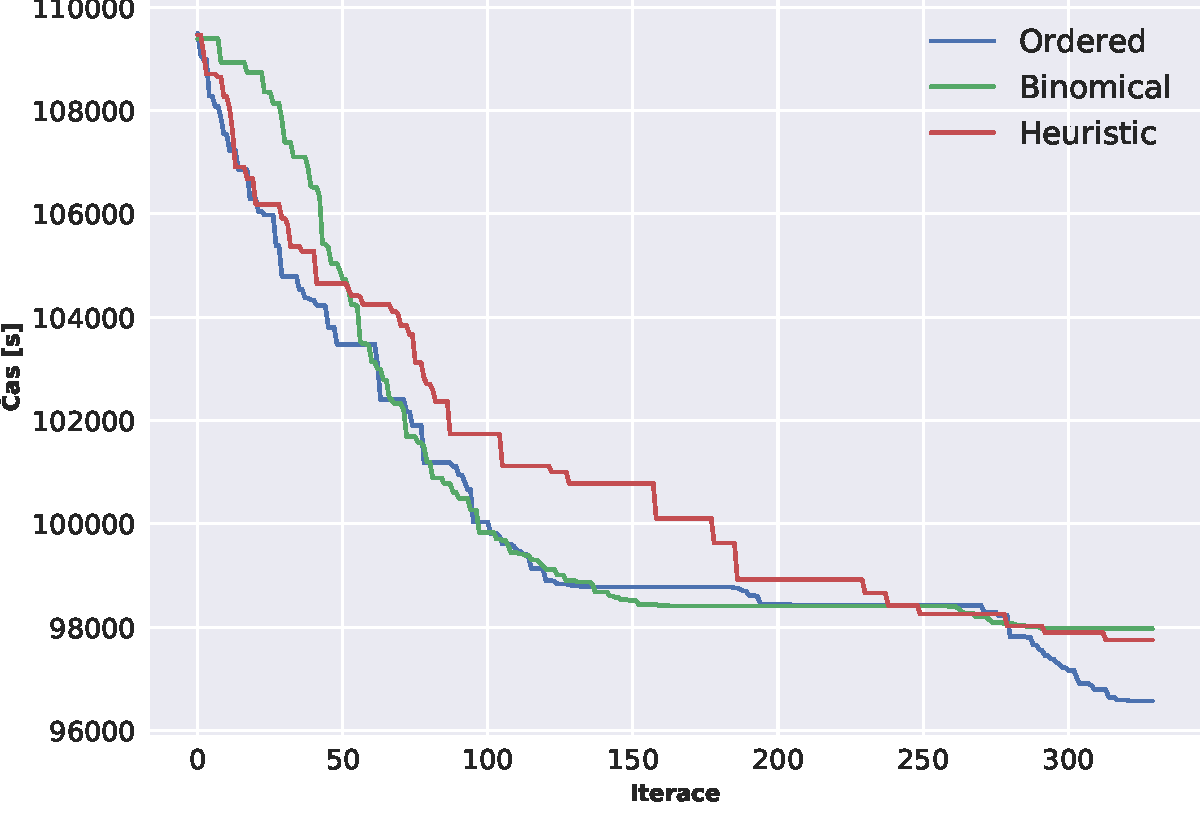
\includegraphics[width=0.99\textwidth]{figures/vyhodnoceni/plotComparisonCrossovers.pdf}
        \caption{Experiment porovnávající různé operátory křížení.}
        \label{fig:compCrossover}
    \end{minipage}\hfill
    \begin{minipage}{0.49\textwidth}
        \centering
        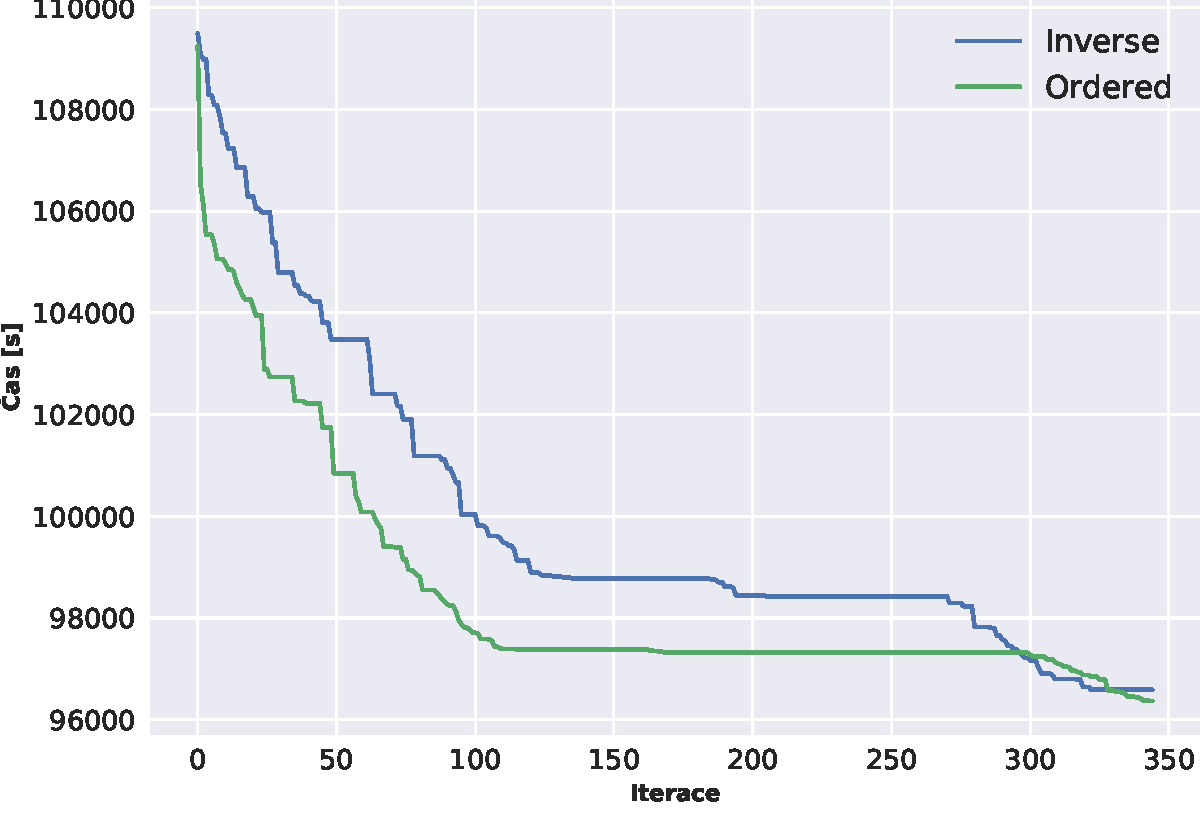
\includegraphics[width=1\textwidth]{figures/vyhodnoceni/plotComparisonMutations.pdf}
        \caption{Experiment porovnávající různé operátory mutace.}
        \label{fig:compMutation}
    \end{minipage}\hfill
\end{figure*}
\begin{figure*}[t]
    \begin{minipage}{0.49\textwidth}
        \centering
        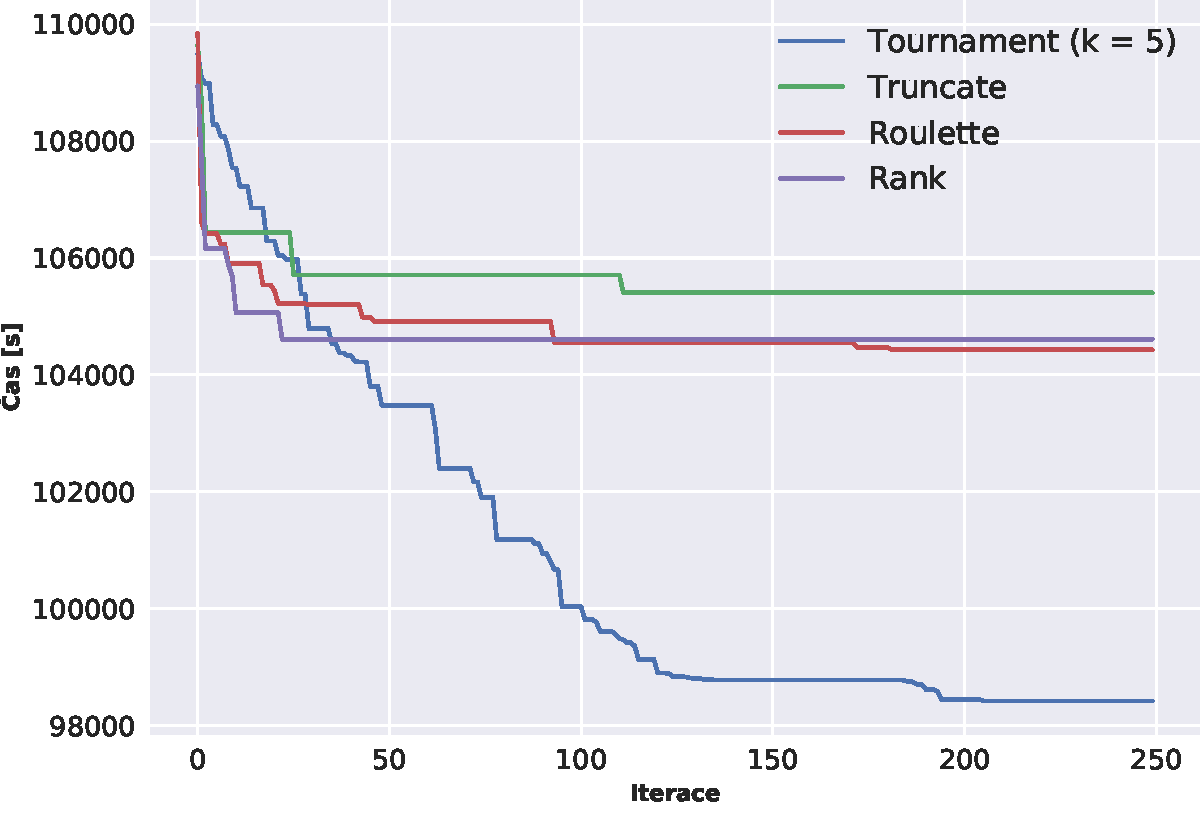
\includegraphics[width=0.99\textwidth]{figures/vyhodnoceni/plotComparisonSelections.pdf}
        \caption{Experiment porovnávající různé operátory selekce.}
        \label{fig:compSelection}
    \end{minipage}\hfill
    \begin{minipage}{0.49\textwidth}
        \centering
        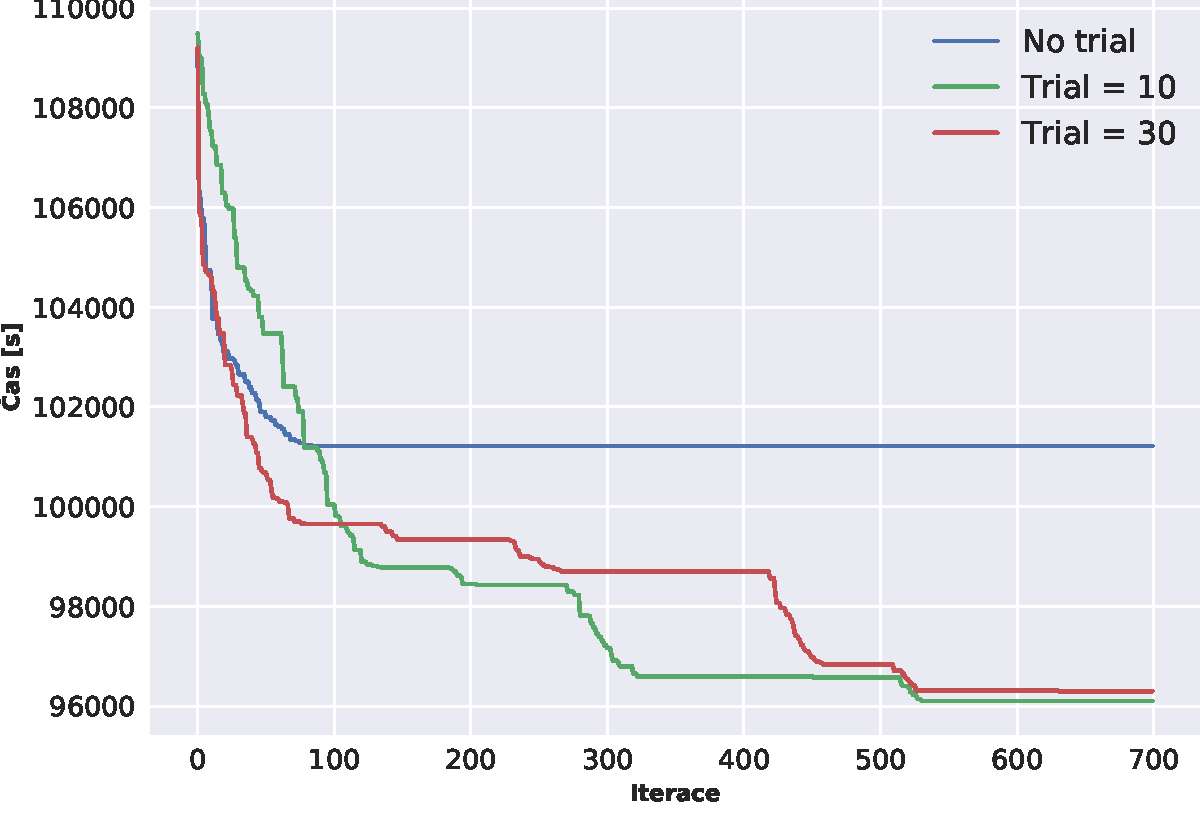
\includegraphics[width=1\textwidth]{figures/vyhodnoceni/plotComparisonTrials.pdf}
        \caption{Experiment porovnávající různé hodnoty $trial$.}
        \label{fig:compTrial}
    \end{minipage}\hfill
\end{figure*}
\begin{figure*}[t]
    \begin{minipage}{0.49\textwidth}
        \centering
        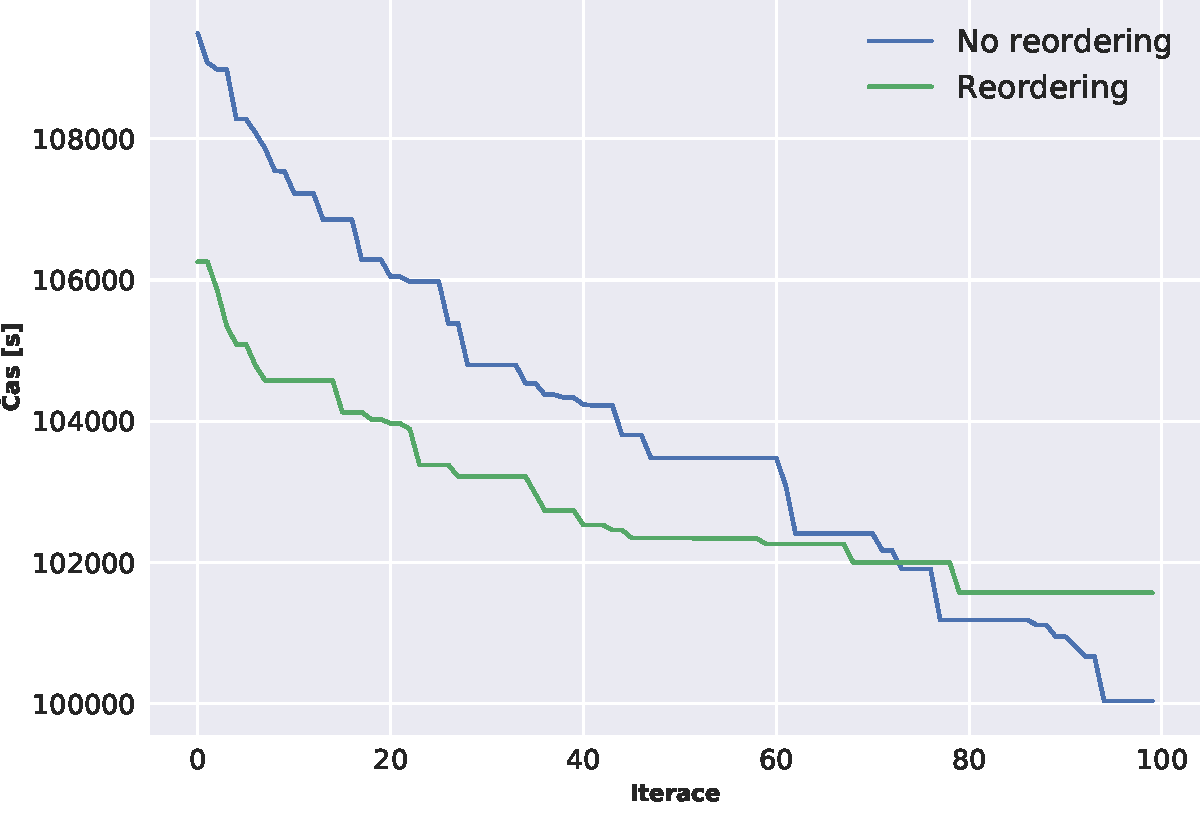
\includegraphics[width=0.99\textwidth]{figures/vyhodnoceni/plotComparisonReordering.pdf}
        \caption{Experiment porovnávající použití uspořádávání a bez použití uspořádávání.}
        \label{fig:compReordering}
    \end{minipage}\hfill
    \begin{minipage}{0.49\textwidth}
        \centering
        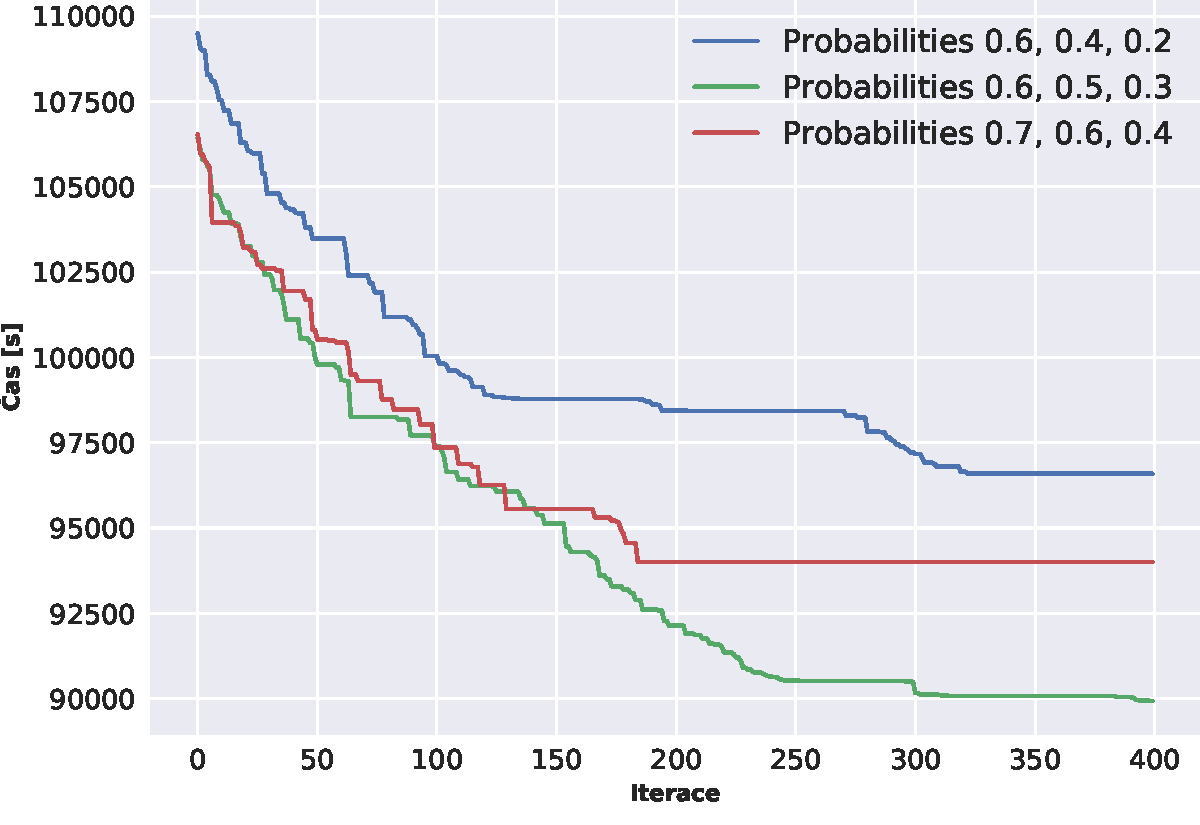
\includegraphics[width=1\textwidth]{figures/vyhodnoceni/plotComparisonParams.pdf}
        \caption{Experiment porovnávající různé pravděpodobnosti provedení křížení a mutace.}
        \label{fig:compParams}
    \end{minipage}\hfill
\end{figure*}

\paragraph{Změna parametrů a vah}
Každý z nástrojů poskytuje bohatou nabídku konfigurací. U~simulátoru je možné například zrychlovat/zpomalovat dopravníky, pracovníky či příchody objednávek. U~těchto hodnot je však vhodné nechat realistickou konfiguraci pro co největší přiblížení izomorfismu s reálným systémem. Optimalizátor umožňuje mimo obecné parametry jako ukládání vah také nastavení různých parametrů evolučních algoritmů. Bylo experimentováno s různými funkcemi pro křížení, mutaci, selekci a dalšími parametry, což značně ovlivňovalo optimalizaci. Pomocí experimentů bylo zjištěno, že nejlepších výsledků dosahuje právě genetický algoritmus a byla nalezena jeho optimální konfigurace, kterou lze najít v tabulce \ref{tab:nejConfig} a v XML souboru přiloženému k aplikaci, aby si jej uživatelé mohli jednoduše načíst. Grafické porovnání lze vidět na snímcích \ref{fig:compCrossover} až \ref{fig:compParams}.

\subsection{Průběh optimalizace}
Ačkoli operace prováděné v evolučních algoritmech jsou zpravidla velmi jednoduchého rázu, v případě této práce velké množství jedinců implikovalo velké množství potřebných simulací a tedy potřebu vysokého výpočetního výkonu pro dosažení rozumné doby optimalizace komplexnějších modelů skladu. Tento problém byl z části řešen tvorbou konfigurovatelného počtu procesů provádějící simulace paralelně~(\ref{section:sim_multithreaded}) a~\uv{eliminací} duplicitních jedinců~(\ref{section:sim_duplicit_jedinci}), avšak stále byla optimalizace na osobním počítači velmi pomalá, nehledě na potřebu neustálého napájení. Z těchto důvodů bylo využito výpočetních zdrojů MetaCentra~\cite{metacentrum}.

MetaCentrum je virtuální organizace poskytující bezplatné výpočetní a úložné kapacity pro členy akademické obce. Uživatelé si mohou na čelním uzlu připravit data a požádat o~naplánování úlohy pomocí PBS (\emph{Portable batch system}). Úlohy lze tvořit buď interaktivní nebo automatizované, ty však vyžadují dávkový soubor. Po přidělení požadovaných prostředků (s většími nároky na zdroje roste i doba než jsou prostředky přiděleny) je úloha spuštěna na jednom z výpočetních uzlů. Požádat o výpočetní zdroje a spuštění úlohy definované dávkovým souborem lze následujícím způsobem:
$$\texttt{qsub -l select=1:ncpus=64:mem=1gb:scratch\_local=1gb:walltime=24:00:00 ga.sh}$$
Tento příkaz do fronty vloží požadavek na 64 procesorů, 1GB paměti RAM, 1GB prostoru na disku a dobu alokace těchto prostředků na 24 hodin. Po přidělení prostředků je proveden obsah dávkového souboru \texttt{ga.sh} na výpočetním uzlu -- to zpravidla zahrnovalo nakopírování zdrojových kódů aplikace \emph{Warehouse Manager} na výpočetní uzel, sestavení programu, použití požadovaného konfiguračního souboru a začátek trénování. V konfiguračním souboru bylo možné nastavit počáteční váhy modelu, a nezačínat tak trénování vždy od znovu. V průběhu výpočtu se průběžně podle konfigurace ukládaly váhy (aby nebyly ztraceny dosažené výsledky v případě pádu aplikace) a po dokončení úlohy nakopírování těchto dosažených výsledků zpět na úložiště.

\section{Warehouse Manager}
Grafická aplikace, ve výsledku nazvaná Warehouse Manager disponuje mimo původní účel (t.j. tvorba 2D modelu skladu), také veškerými funkcionalitami implementovanými v rámci této práce. To znamená veškerou kontrolu nad simulátorem, generátorem, pathfinderem i~optimalizátorem. To umožňuje možnost plného využití této práce i technicky méně zdatným jedincům, jako např. logistickým manažerům, zcela bez nutnosti využít příkazovou řádku.

\subsection{Layout aplikace}
Rozložení grafické aplikace bylo vytvořeno za pomoci aplikace \texttt{Qt Designer}: v horní liště lze najít tlačítka pro ovládání, jako např. vytvoření nového modelu skladu, načtení již existujícího modelu ze souboru, atd. Dále se v této liště nachází jednotlivé prvky/zařízení skladu, které může uživatel využít pro vytvoření modelu skladu. Na levé straně aplikace jsou záložky, které slouží pro import, export a náhled dat využívaných jednotlivými nástroji, jako jsou (zleva): objednávky pro trénování a testování, produkty a lokace se sloty, které mohou obsahovat i aktuální alokaci produktů do daných slotů. Vpravo jsou opět záložky, které slouží pro přepínání mezi jednotlivými nástroji. Každý z těchto čtyř nástrojů má ve své záložce následující části:

\begin{itemize}
    \item \textbf{Konfigurace} -- Zde jsou veškeré parametry, které daný nástroj poskytuje a lze je předvyplnit konfiguračním souborem, či je exportovat do XML.
    \item \textbf{Statistiky} -- Zde jsou obsaženy grafy, do kterých jsou postupně doplňovány hodnoty produkované daným nástrojem.
    \item \textbf{Řízení} -- Poskytuje tlačítka pro kontrolu jednotlivých nástrojů, jako je spuštění či zastavení. Ve chvíli, kdy je spuštěn jeden z uvedených nástrojů, jsou veškerá kontrolní tlačítka, stejně tak úprava modelu skladu, zakázána. A to aby uživatel nijak nenarušil běh daného nástroje. Naopak se povolí tlačítko pro zastavení běhu nástroje. Zastavení nebo dokončení práce nástrojem opět povolí úpravu modelu skladu a veškerá tlačítka.
\end{itemize}

Uprostřed aplikace je plocha určená pro tvorbu a manipulaci s modelem skladu. Cílem této plochy je poskytnout úplný a intuitivní 2D editor poskytující různé druhy skladových prvků a manipulaci s nimi. Ve výsledku editor (mimo jiné) umožňuje:

\begin{itemize}
    \item Měřítko vůči reálnému světu.
    \item Změnu velikosti, pozice a rotaci prvků.
    \item Propojování skladových prvků pomocí portů.
    \item Hromadnou selekci a kopírování prvků.
    \item Zobrazení podrobných informací o prvku.
    \item Uložení modelu skladu do souboru a načtení ze souboru.
    \item Přiblížení a oddálení scény/modelu skladu\footnote{Inspirováno \url{https://stackoverflow.com/a/19114517/8254699}.}.
\end{itemize}

\subsection{Tvorba modelu skladu}
\label{sec:uiModelSkladu}
Uživatel, který chce aplikaci plně využít ve svůj prospěch, musí být schopen vytvořit model skladu dle jeho potřeb. Zejména pro tyto účely byla grafická aplikace navržena, a později doplněna o veškerou ostatní funkcionalitu. Pro implementaci plochy pro tvorbu modelu skladu byla využita grafická scéna (\texttt{QGraphicsScene}\footnote{\url{https://doc.qt.io/qt-5/qgraphicsscene.html}}) a grafický pohled (\texttt{QGraphicsView}\footnote{\url{https://doc.qt.io/qt-5/qgraphicsview.html}}). Do grafické scény jsou postupně umisťovány prvky skladu odvozené od grafických prvků (\texttt{QGraphicsItem}\footnote{\url{https://doc.qt.io/qt-5/qgraphicsitem.html}}), doplňující je o specifickou funkcionalitu. Při implementaci byly využity volně dostupné doplňky \texttt{Qt}: \texttt{QDarkStyleSheet}\footnote{\url{https://github.com/ColinDuquesnoy/QDarkStyleSheet}}, \texttt{QCustomPlot}\footnote{\url{https://www.qcustomplot.com}} a \texttt{QtEditableItems}\footnote{\url{https://github.com/fadyosman/QtEditableItems}}.

\subsubsection{Grafická scéna}
Grafický pohled umožňuje zobrazení grafické scény ve widgetu. Grafická scéna slouží jako kontejner grafických prvků a v kombinaci s grafickým pohledem slouží k vizualizaci takovýchto prvků na 2D povrchu. Pro účely přepsání jistých vlastností grafické scény (jako např. zobrazení kontextového menu) byla tato třída odvozena. Stejně tak grafické prvky, které byly do scény umisťovány, byly odvozeny a velmi značně přepsány pro daný \emph{use-case}. Takovéto odvození umožnilo například vytvoření manipulátorů pro změnu velikosti prvků a také jejich rotaci, viz \ref{fig:uiItemInfo}. Uživatel je na začátku práce dotázán na velikost skladu v metrech. Tyto rozměry jsou interně přepočteny a je vytvořeno ohraničení skladu bílými čarami, mřížkou pro jednodušší manipulaci s prvky a také měřítkem (vlevo nahoře). Délka měřítka je vždy jedna pětina šířky grafické scény, a číslo nad ní udává, kolik metrů ve skutečnosti tato délka (část scény) reprezentuje.

Grafický pohled a scéna byly doplněny mimo jiné také o možnost přibližování a oddalování, bez kterých by byla aplikace jen velmi těžce použitelná. Tohoto lze dosáhnout pomocí přidržení klávesy \texttt{CTRL} a pohybem rolovacího tlačítka myši. Při této akci se také přepočítává měřítko vůči reálnému světu. Pro usnadnění tvorby komplexních modelů skladu byla implementována možnost hromadného označování prvků a následně možnost kopírování a~přemisťování označených prvků, což může velmi usnadnit tvorbu modelu.

\subsubsection{Grafické prvky}
Jak již bylo zmíněno, grafické prvky jsou odvozeny z \texttt{QGraphicsItem}. Poté jsou z této odvozené třídy odvozeny další třídy pro každý typ zařízení, a sice:

\begin{itemize}
    \item \texttt{UiWarehouseItemLocation\_t} -- Reprezentuje lokace.
    \item \texttt{UiWarehouseItemConveyor\_t} -- Reprezentuje dopravníky.
    \item \texttt{UiWarehouseItemGate\_t} -- Reprezentuje vstupní a výstupní brány skladu.
\end{itemize}

Veškeré grafické prvky jsou reprezentovány jako ukazatele na dynamicky alokovanou paměť, tzv. \uv{hromadu} (ang. \emph{heap}), a to z důvodu aby grafické prvky existovaly i po opuštění rozsahu části programu, kde jsou vytvořeny. O uvolnění paměti se poté starají mechanismy frameworku Qt díky specifikaci rodičovských prvků, až po hlavní okno. Tzn. při destrukci rodiče jsou uvolněni veškeří následníci, poté jejich následníci, a tak dále. Jednotlivé třídy jsou rozšířeny o funkcionalitu specifickou pro dané zařízení skladu. Např. lokace je rozšířena o mřížku slotů, tedy kontejner instancí třídy \texttt{UiWarehouseSlot\_t} atd.

Propojování grafických prvků lze provádět na základě portů -- \texttt{UiWarehousePort\_t} (oranžové šipky na každém z prvků, viz \ref{fig:uiItemInfo}). Po připojení daného portu k jinému se tyto spojené porty skryjí a ukáží se opět při odpojení prvku. Každé ze zařízení má jiný počet portů, dle jeho způsobu použití.

\begin{figure}[t]
    \centering
    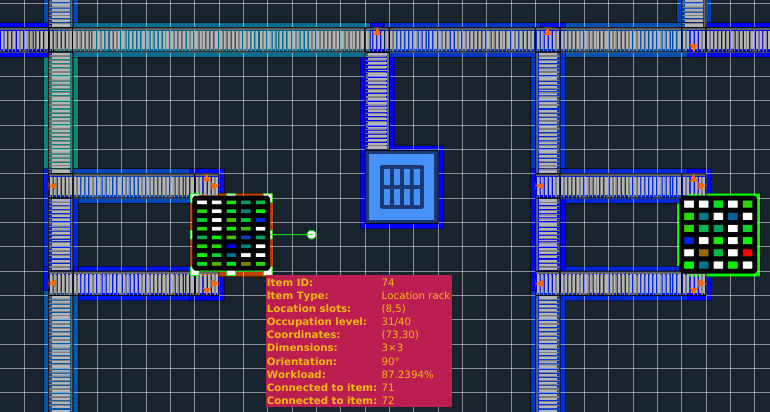
\includegraphics[width=0.95\linewidth]{figures/implementace/UI_model_info.png}
    \caption{Zobrazení informací o zařízení skladu pomocí najetí kurzorem (přesně se jedná o lokaci). Dále lze na snímku vidět porty sloužící k propojování prvků (oranžové šipky) a nakonec také manipulátory, pomocí kterých lze vybraný prvek rotovat a měnit jeho velikost.}
    \label{fig:uiItemInfo}
\end{figure}


Informace o~grafickém prvku lze zobrazit pomocí najetí myší na daný prvek, viz \ref{fig:uiItemInfo}. V~zobrazené tabulce lze najít veškeré informace o~prvku, ať už jde o~pozici, velikost a~natočení, nebo specifické informace jako zatížení prvku nebo úroveň obsazenosti lokace.

\subsubsection{Serializace modelu skladu}
Model skladu může být poměrně komplexní, a~jeho opětovné vytváření při každém spuštění by nedávalo smysl. Proto je možné model serializovat (uložit) do souboru ve formátu XML (pomocí knihovny \texttt{libxml2}), a také jej ze souboru deserializovat (načíst) do grafického rozhraní. Velmi jednoduchý příklad lze vidět na následujícím výpisu.
\newpage
\lstset{
    language=xml,
    tabsize=3,
    %frame=lines,
    caption=Test,
    label=code:sample,
    frame=shadowbox,
    rulesepcolor=\color{gray},
    xleftmargin=20pt,
    framexleftmargin=15pt,
    keywordstyle=\color{blue}\bf,
    commentstyle=\color{OliveGreen},
    stringstyle=\color{red},
    numbers=left,
    numberstyle=\tiny,
    numbersep=5pt,
    breaklines=true,
    showstringspaces=false,
    basicstyle=\footnotesize,
    emph={food,name,price},emphstyle={\color{magenta}}}
    \lstinputlisting[caption={Serializovaný model skladu ve formátu XML. První element obsahuje informace o layoutu, jako je výška, šířka a kolik jeden metr představuje bodů ve scéně. Další element představuje dopravník i s informacemi, kde se ve scéně nachází, jak je velký a jak je natočený. Následuje lokace, která mimo pozici apod. obsahuje také informaci o slotech. Následuje jediný propoj vytvořený mezi těmito dvěma prvky.}]{data/layout.xml}

    
\section{Moduly programu}
V této sekci jsou velmi krátce popsány jednotlivé moduly programu, které jsou v různé míře využity všemi implementovanými nástroji. Operátor rozsahu platnosti zde identifikuje jednotlivé jmenné prostory, ve kterých jsou moduly uloženy:

\begin{itemize}
    \item \texttt{whm::ConfigParser\_t} -- Tento modul slouží pro serializaci a de-serializaci konfiguračních souborů v XML, a umožňuje získávání konfiguračních hodnot pomocí šablonové metody.
    \item \texttt{whm::Logger\_t} -- Komplexní modul pro zaznamenávání běhu aplikace na výstup či do souboru.
    \item \texttt{whm::utils::*} -- Utility (šablonové funkce) plošně využívané v celé aplikaci.
    \item \texttt{whm::WarehouseDataGenerator\_t} -- Modul který obstarává generování zákaznických objednávek.
    \item \texttt{whm::WarehouseSimulatorSIMLIB\_t} -- Modul který obstarává simulaci skladu pomocí knihovny \texttt{SIMLIB/C++}.
    \item \texttt{whm::WarehousePathFinder\_t} -- Modul, který rekurzivně vyhledá veškeré cesty ve skladu, uloží do vhodné datové struktury a umožňuje nalezení nejkratší cesty mezi lokacemi, apod.
    \item \texttt{whm::WarehousePathFinderACO\_t} -- Implementace mravenčího algoritmu pro nalezení nejkratší cesty objednávky skrze celý sklad.
    \item \texttt{whm::WarehouseOptimizer\{Base|GA|DE|ABC|PSO|SLAP|RAND\}\_t} -- Implementace\newline čtyř evolučních algoritmů v diskrétním prostoru, metodiky SLAP, náhodného prohledávání a bázové třídy, ze které jsou všechny optimalizátory odvozeny. Optimalizátory využívají definici řešení problému definovaného v modulu \texttt{whm::Solution\_t}.
    \item \texttt{whm::WarehouseOrder\_t} -- Modul implementující zákaznickou objednávku.
    \item \texttt{whm::WarehouseOrderLine\_t} -- Modul implementující část (položku) zákaznické objednávky.
    \item \texttt{whm::WarehouseLocationRack\_t} -- Modul implementující lokaci, která se skládá ze slotů a jsou v ní uloženy produkty.
    \item \texttt{whm::WarehouseLocationSlot\_t} -- Modul implementující sloty, ze kterých sestává lokace.
    \item \texttt{whm::WarehousePort\_t} -- Modul implementující port pomocí kterého lze propojovat jednotlivé prvky.
    \item \texttt{whm::WarehouseConnection\_t} -- Modul implementující propojení prvků ve skladu.
    \item \texttt{whm::WarehouseItem\_t} -- Modul implementující prvek/zařízení skladu.
    \item \texttt{whm::WarehouseLayout\_t} -- Modul poskytující \emph{singleton}, který obsahuje veškeré důležité informace o celém skladu.
    \item \texttt{whm::gui::*} -- Grafická nástavba textového klienta (souborů výše), která sestává z~cca. 15 modulů, mimo jiné také z vláken, které složí k provádění náročných operací jako je např. optimalizace -- aby neblokovaly hlavní smyčku (grafické okno). Dále pak z odvozených grafických prvků, scény, apod. Pokud je definován symbol \texttt{WHM\_GUI}, jsou některé moduly v seznamu nahoře doplněny o zpětné volání do grafického rozhraní. 
\end{itemize}



\chapter{Vyhodnocení účinnosti vytvořených nástrojů}
\label{vyhodnoceniNastroju}
Cílem této práce bylo zejména optimalizovat sklad tak, aby se maximalizovala propustnost skladu, tedy počet zpracovaných objednávek za jednotku času. To lze chápat také jako zpracování daných objednávek v co nejkratším možném čase. Vyhodnocení je rozděleno na tři části: optimalizaci rozložení produktů, cesty a nakonec jejich kombinaci.

\section{Optimalizace rozložení produktů}
Jak již bylo zmíněno, při optimalizaci tohoto problému se minimalizuje doba potřebná ke zpracování sady objednávek. Na grafu na obrázku~\ref{fig:vyhodnoceniGrafTrain} lze vidět průběh optimalizace pomocí evolučních algoritmů na problému rozřazení $150$ produktů do $200$ slotů, což lze vyjádřit jako kombinatorický problém:
\begin{equation*}
    \label{eq:optVariace}
    V_{150}(200) = \frac{200!}{50!} = 2.593067\text{e}+310.
\end{equation*}
Dále je na grafu vidět také průběh náhodného prohledávání prostoru (\texttt{RAND}) a klasické metodiky (\texttt{Battista a spol.}) použité v práci~\cite{slapSeacomp} -- tato metodika je jednokrokový výpočet mapující nejčastěji kupované produkty do nejvýhodnějších slotů, a proto je konstantní. Nejlépe si vedl genetický algoritmus, kterému se povedlo snížit dobu potřebnou ke zpracování $1000$ objednávek téměř na polovinu ($57\%$). Stejnou optimalizaci avšak v časové doméně (\emph{trade-off} úspěšnosti a času) lze vidět na obrázku~\ref{fig:vyhodnoceniGrafTrainCas}. Vyhodnocení optimalizovaných modelů na testovací sadě vždy cca. odpovídalo úrovni optimalizace na trénovací sadě objednávek. Při kombinatorickém nárůstu možných řešení a při zachování nastavení optimalizátoru a délky optimalizace se kvalita optimalizace snižuje, viz obrázek~\ref{fig:vyhodnoceniPorovnaniOpt} a obrázek~\ref{fig:vyhodnoceniPorovnaniOpt7501000}.

Při analýze průběhů trénování lze vidět, že náhodné prohledávání je z pohledu optimalizace téměř bezvýznamné. Genetický algoritmus velmi rychle konverguje na začátku, ale zhruba od iterace 400 už se vůbec nezlepšuje. Další iterace by tomuto algoritmu tedy už nejspíše nepomohly. Na druhou stranu algoritmus umělých včelstev, optimalizace rojem částic a diferenční evoluce konvergují mnohem pomaleji a při dalších iteracích by se výsledek nejspíše dále lehce zlepšoval. Algoritmus optimalizace rojem částic je z uvedených evolučních algoritmů pro tuto problematiku nejméně vhodný a jako jediný dosahuje horších výsledků, než klasická metoda Battista a spol~\cite{slapSeacomp}. Nejlépe tedy dle očekávání dopadl genetický algoritmus, a sice na všech instancích problému, kterému se podařilo dobu potřebnou pro zpracování objednávek snížit téměř na polovinu.

Vzhledem k tomu, že z porovnání algoritmů pro řešení problematiky SLAP vyšel jako nejlepší genetický algoritmus, pro další experimenty s optimalizací rozložení produktů byl využíván už pouze tento algoritmus. Na snímcích \ref{fig:compCrossover} až \ref{fig:compParams} lze vidět experimenty s různými parametry genetického algoritmu. Z těchto experimentů bylo možné najít nejlepší konfiguraci optimalizátoru, která byla nadále používána a kterou lze vidět v tabulce~\ref{tab:nejConfig}.

\begin{figure*}[t]
    \centering
    \begin{minipage}{0.49\textwidth}
        \centering
        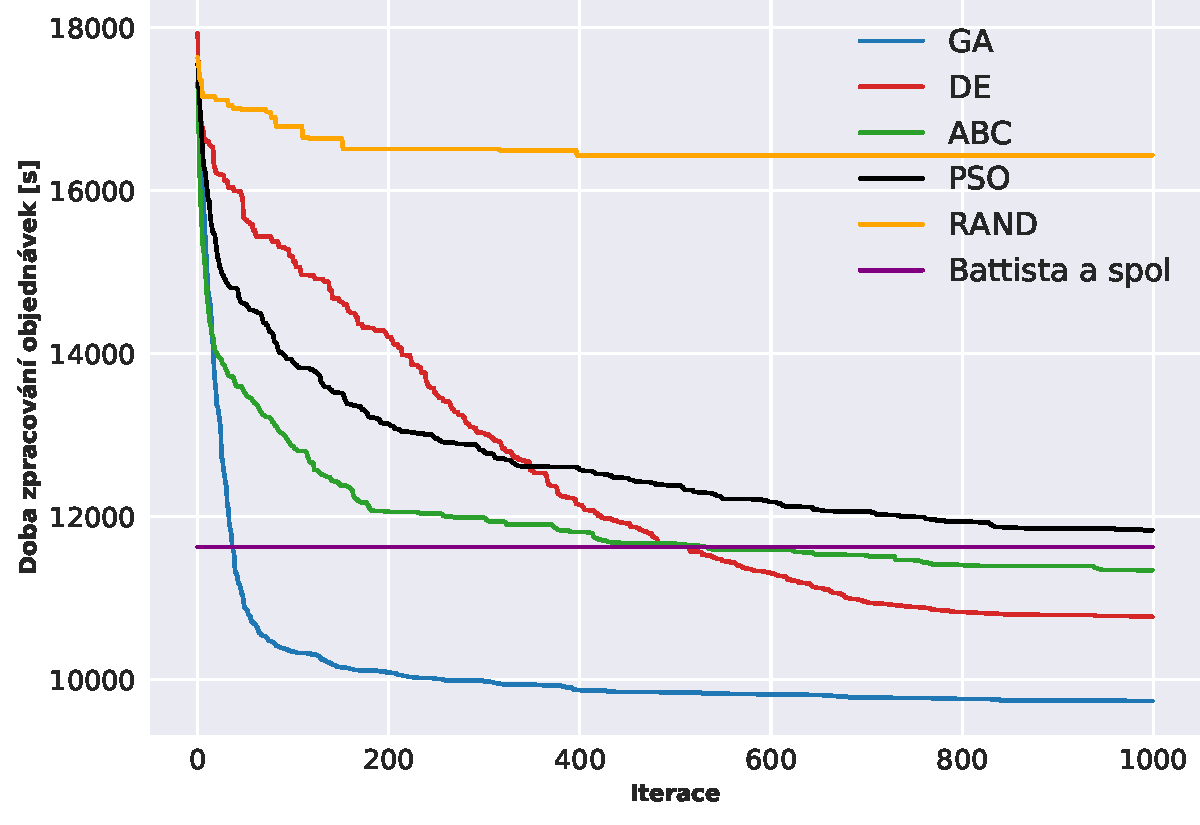
\includegraphics[width=0.99\textwidth]{figures/vyhodnoceni/plotComparisonTrain.pdf}
        \caption{Graf průběhu optimalizace pomocí čtyř evolučních algoritmů, metodiky Battista a spol.~\cite{slapSeacomp} a náhodného prohledávání. Ve všech případech byl použit stejný model skladu (který lze vidět na snímku~\ref{fig:UI_simulator}) a stejné trénovací objednávky. Na vodorovné ose jsou iterace algoritmu a na svislé ose je doba potřebná pro zpracování sady trénovacích objednávek v sekundách. Jedná se o aritmetický průměr \textbf{pěti} běhů na metodu.}
        \label{fig:vyhodnoceniGrafTrain}
    \end{minipage}\hfill
    \begin{minipage}{0.49\textwidth}
        \centering
        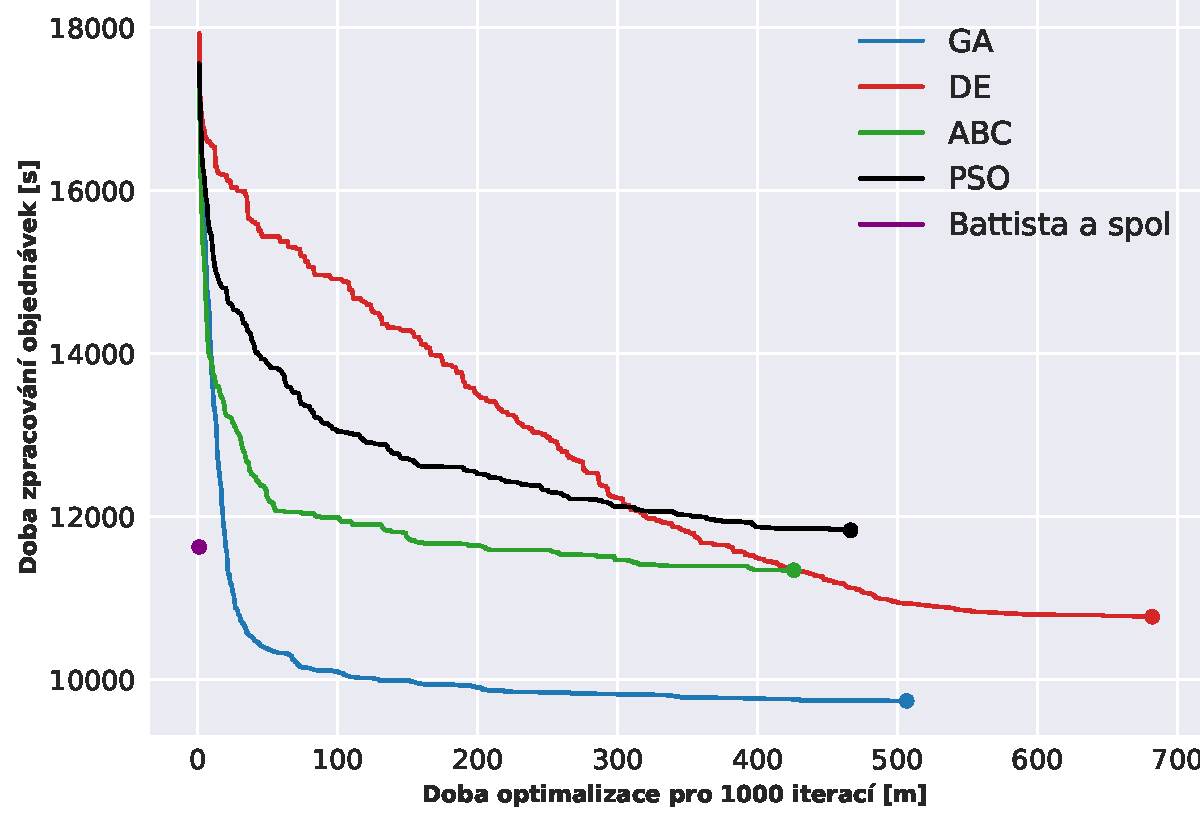
\includegraphics[width=1\linewidth]{figures/vyhodnoceni/plotComparisonTrainTime.pdf}
        \caption{Průběh optimalizace z grafu na obrázku~\ref{fig:vyhodnoceniGrafTrain} v časové doméně, tzn. jak dlouho trvalo 1000 iterací jednotlivých metod. Pokud bychom nebrali v potaz genetické algoritmy, nejvhodnější by byla diferenční evoluce, pokud bychom však měli na optimalizace méně než 400 minut, vhodnější by byl algoritmus umělých včelstev a do 300 minut by vycházel lépe dokonce i algoritmus optimalizace rojem částic.}
        \label{fig:vyhodnoceniGrafTrainCas}
    \end{minipage}\hfill
\end{figure*}

\begin{figure*}[t]
    \centering
    \begin{minipage}{0.49\textwidth}
        \centering
        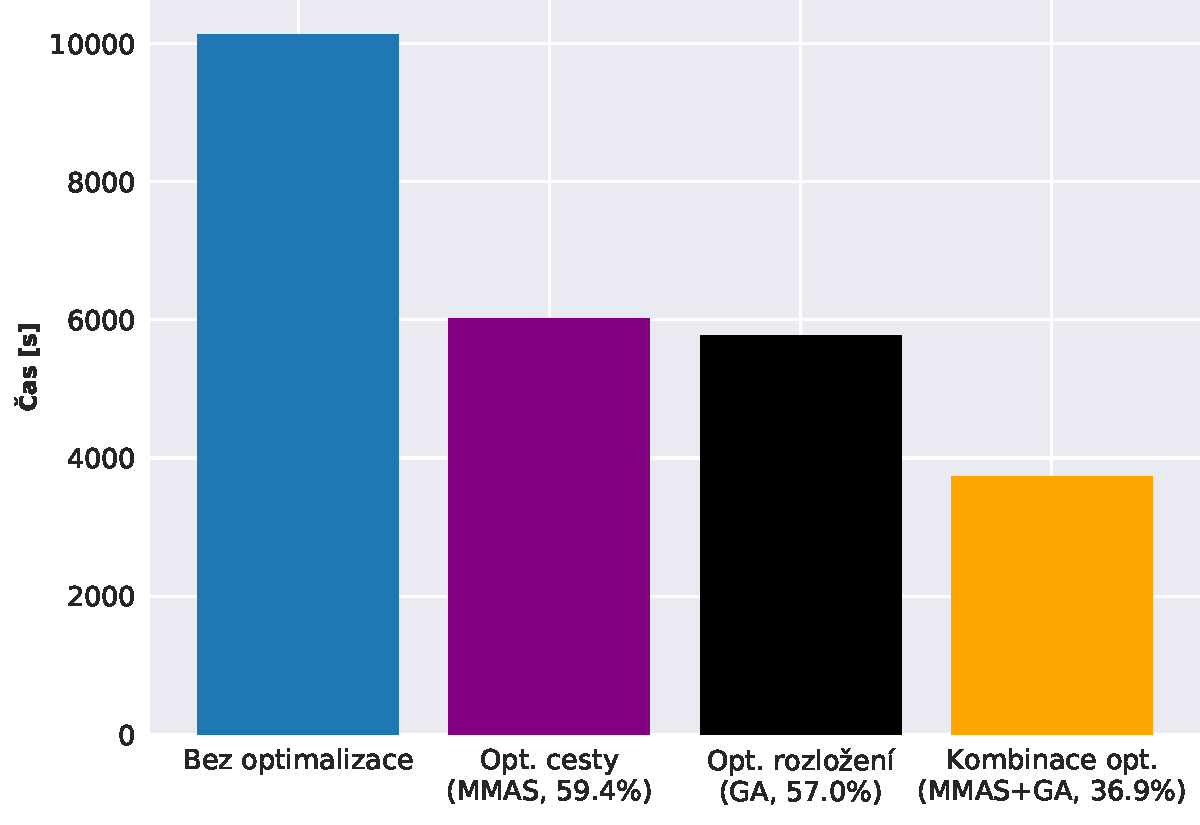
\includegraphics[width=0.99\textwidth]{figures/vyhodnoceni/plotOptimizersComparison.pdf}
        \caption{Sloupcový graf porovnávající optimalizaci cesty pomocí $\mathcal{M}\!\!\mathcal{M}$AS, optimalizaci rozložení produktů pomocí genetického algoritmu a nakonec jejich kombinaci (sklad $200$ produktů, $400$ slotů).}
        \label{fig:vyhodnoceniPorovnaniOpt}
    \end{minipage}\hfill
    \begin{minipage}{0.49\textwidth}
        \centering
        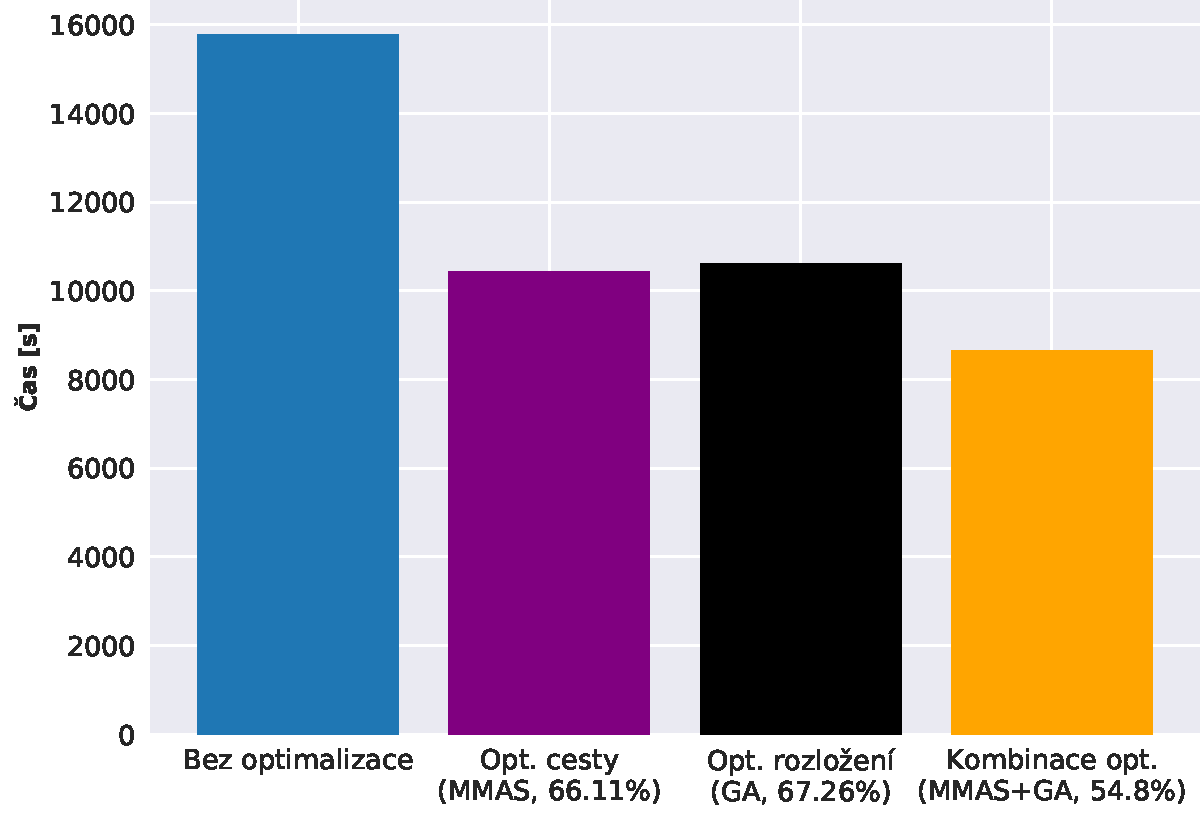
\includegraphics[width=0.99\textwidth]{figures/vyhodnoceni/plotOptimizersComparison7501000.pdf}
        \caption{Sloupcový graf porovnávající optimalizaci cesty pomocí $\mathcal{M}\!\!\mathcal{M}$AS, optimalizaci rozložení produktů pomocí genetického algoritmu a nakonec jejich kombinaci (sklad $750$ produktů, $1000$ slotů).}
        \label{fig:vyhodnoceniPorovnaniOpt7501000}
    \end{minipage}\hfill
\end{figure*}
\begin{figure}[t!]
    \centering
    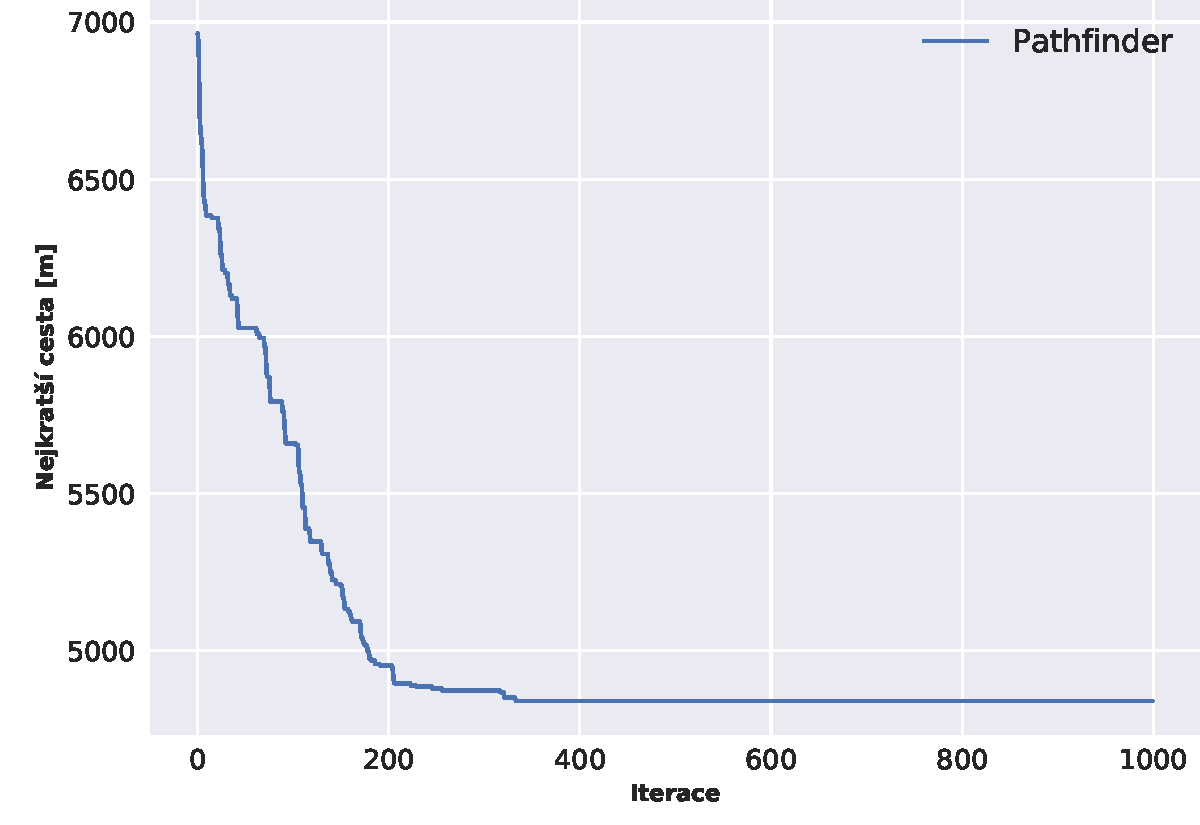
\includegraphics[width=0.7\linewidth]{figures/vyhodnoceni/plotPathFinder.pdf}
    \caption{Graf průběhu hledání optimální cesty pomocí algoritmu $\mathcal{M}\!\!\mathcal{M}$AS na velkém skladu. Jedná se o aritmetický průměr pěti běhů.}
    \label{fig:vyhodnoceniPathFinder}
\end{figure}

\section{Optimalizace cesty}
V rámci této práce byl jako doplněk implementován také nástroj pathfinder, který pomocí mravenčího algoritmu dokáže nalézt optimální cestu objednávky skrze sklad. Na obrázku~\ref{fig:vyhodnoceniPathFinder} lze vidět průběh hledání optimální cesty na skladu o velikosti $200$ lokací, což už je z hlediska skladových politik více než obrovský sklad a tedy nemá význam řešit tento problém pro větší modely skladu. Algoritmus v závislosti na konfiguraci dokáže nalézt optimální řešení (cestu s nejkratší vzdáleností) pro zmíněný sklad do $400$ iterací algoritmu. U skladů typických velikostí je optimální cesta nalezena maximálně do $100$ iterací algoritmu.

\section{Kombinace optimalizací}
Nástroj pathfinder lze použít v rámci simulátoru pro hledání optimálních cest pro objednávky. Vzhledem k tomu, že optimalizátor rozložení používá simulátor pro aproximaci kvality řešení, lze použít všechny tři nástroje zároveň a optimalizovat jednak rozložení produktů a zároveň délku cesty. Na grafu~\ref{fig:vyhodnoceniPorovnaniOpt} lze vidět porovnání (na problému $200$ produktů, $400$ slotů): neoptimalizovaný sklad, nejlepší dosažené výsledky samostatných optimalizací a nakonec kombinace těchto optimalizací. Jak lze vidět, kombinací těchto optimalizátorů lze dosáhnout ještě lepších výsledků, avšak za velice vysokou cenu doby trénování -- optimalizace cesty trvá jednotky minut, optimalizace rozložení jednotky hodin (viz graf na obrázku~\ref{fig:vyhodnoceniGrafTrainCas}) a jejich kombinace pak desítky hodin. Kombinace optimalizací trvající desítky hodin už není v souladu s fungováním moderních skladů, které musí být schopny relativně rychle reagovat na změny požadavků na trhu.



\chapter{Závěr}
Práce měla za úkol vytvořit nástroj, který bude schopen optimalizovat fungování skladu za účelem zvýšení jeho propustnosti. Důležitou podmínkou byla nezávislost optimalizace na modelu skladu (tj. uživatel jej může vytvořit dle svých potřeb), čehož bylo dosaženo za pomoci grafického editoru a realistické simulace. Dále bylo třeba vytvořit generátor syntetických objednávek kvůli citlivosti zákaznických dat a nakonec kvantitativně vyhodnotit dosažené výsledky.

Nástroj pathfinder dokáže nalézt optimální cestu skrze sklad v relativně malém počtu iterací algoritmu a zrychlení zpracování objednávek je téměř dvojnásobné -- $\textbf{59.4\%}$. Stejně tak optimalizátor rozložení produktů dokáže téměř dvojnásobně zrychlit zpracování všech objednávek -- $\textbf{57\%}$, avšak doba pro natrénování je zde značně delší. Kombinací těchto dvou přístupů zároveň pak lze dosáhnout ještě lepších výsledků, avšak za cenu velmi dlouhé optimalizace. Při kombinatorickém nárůstu možných řešení a při zachování nastavení optimalizátoru a délky optimalizace se kvalita optimalizace rozložení snižuje -- nejvýše však~o~$\textbf{10\%}$.

Přínosem této práce je úplný grafický nástroj, jenž dosahuje velmi dobrých výsledků a poskytuje mnoho užitečných funkcí v oblasti skladového hospodářství. Dále tato práce přináší novou metodu k řešení problematiky SLAP a sice kombinaci dvou \emph{state of the art} technik a nakonec přináší nové optimalizační kritérium v kontextu SLAP -- celkovou dobu zpracování sady objednávek.

V budoucnu by bylo možné rozšířit práci o nástroj schopný generovat optimální rozložení skladu na základě uživatelem definovaných podmínek, a to za pomoci CGP (kartézského genetického programování).
  \fi
  
  % Kompilace po částech (viz výše, nutno odkomentovat)
  % Compilation piecewise (see above, it is necessary to uncomment it)
  %\subfile{projekt-01-uvod-introduction}
  % ...
  %\subfile{chapters/projekt-05-conclusion}


  % Pouzita literatura / Bibliography
  % ----------------------------------------------
\ifslovak
  \makeatletter
  \def\@openbib@code{\addcontentsline{toc}{chapter}{Literatúra}}
  \makeatother
  \bibliographystyle{bib-styles/Pysny/skplain}
\else
  \ifczech
    \makeatletter
    \def\@openbib@code{\addcontentsline{toc}{chapter}{Literatura}}
    \makeatother
    \bibliographystyle{bib-styles/Pysny/czplain}
  \else 
    \makeatletter
    \def\@openbib@code{\addcontentsline{toc}{chapter}{Bibliography}}
    \makeatother
    \bibliographystyle{bib-styles/Pysny/enplain}
  %  \bibliographystyle{alpha}
  \fi
\fi
  \begin{flushleft}
  \bibliography{xkocic01-DP-20-literatura-bibliography}
  \end{flushleft}

  % vynechani stranky v oboustrannem rezimu
  % Skip the page in the two-sided mode
  \iftwoside
    \cleardoublepage
  \fi

  % Prilohy / Appendices
  % ---------------------------------------------
  \appendix
\ifczech
  \renewcommand{\appendixpagename}{Přílohy}
  \renewcommand{\appendixtocname}{Přílohy}
  \renewcommand{\appendixname}{Příloha}
\fi
\ifslovak
  \renewcommand{\appendixpagename}{Prílohy}
  \renewcommand{\appendixtocname}{Prílohy}
  \renewcommand{\appendixname}{Príloha}
\fi
%  \appendixpage

% vynechani stranky v oboustrannem rezimu
% Skip the page in the two-sided mode
%\iftwoside
%  \cleardoublepage
%\fi
  
\ifslovak
%  \section*{Zoznam príloh}
%  \addcontentsline{toc}{section}{Zoznam príloh}
\else
  \ifczech
%    \section*{Seznam příloh}
%    \addcontentsline{toc}{section}{Seznam příloh}
  \else
%    \section*{List of Appendices}
%    \addcontentsline{toc}{section}{List of Appendices}
  \fi
\fi
  \startcontents[chapters]
  \setlength{\parskip}{0pt} 
  % seznam příloh / list of appendices
  % \printcontents[chapters]{l}{0}{\setcounter{tocdepth}{2}}
  
  \ifODSAZ
    \setlength{\parskip}{0.5\bigskipamount}
  \else
    \setlength{\parskip}{0pt}
  \fi
  
  % vynechani stranky v oboustrannem rezimu
  \iftwoside
    \cleardoublepage
  \fi
  
  % Přílohy / Appendices
  \ifenglish
    \input{projekt-30-prilohy-appendices-en}
  \else
    % Tento soubor nahraďte vlastním souborem s přílohami (nadpisy níže jsou pouze pro příklad)
% This file should be replaced with your file with an appendices (headings below are examples only)

% Umístění obsahu paměťového média do příloh je vhodné konzultovat s vedoucím
% Placing of table of contents of the memory media here should be consulted with a supervisor

\chapter{Obsah přiloženého paměťového média}

\begin{itemize}
    \item \texttt{src} -- Zdrojové kódy vytvořené aplikace \texttt{WarehouseManager}.
    \item \texttt{utils} -- Skripty používané v~průběhu práce, zejména ke trénování na výpočetním clusteru a~k~vyhodnocení.
    \item \texttt{doc} -- Plakát použitý k prezentaci této práce a video prezentující dosažené výsledky.
    \item \texttt{README} -- Více obsáhlá příručka v~anglickém jazyce (ve formátu \texttt{md} -- \emph{markdown}).
    \item \texttt{report} -- Adresář obsahující zdrojové kódy tohoto dokumentu ve formátu \LaTeX, a~také jejich přeloženou verzi ve formátu \texttt{PDF}.
\end{itemize}


\chapter{Manuál}

Sestavení a použití aplikace \texttt{WarehouseManager} na linuxovém OS:

\begin{enumerate}
    \item Instalace grafického frameworku \texttt{Qt5} a knihovny \texttt{SIMLIB/C++} dle jejich dokumentace.
    \item Spuštění kompilace pomocí příkazu \texttt{make} v kořenovém adresáři projektu.
    \item Nastavení konfigurace v grafickém rozhraní nebo v souborech v adresáři \texttt{cfg/}.
    \item Po úspěšné kompilaci lze provést spuštění nástrojů následovně:
    \begin{verbatim}
        ./whm_gui
        ./whm_gen -o orders.xml -a articles.csv
        ./whm_sim -o orders_test.xml  -i locations.csv \
                  -l layout.xml
        ./whm_paf -o orders_test.xml  -i locations.csv \
                  -l layout.xml [-s]
        ./whm_opt -o orders_train.xml -i locations.csv \
                  -l layout.xml -a articles.csv -O 1-6
    \end{verbatim}
    \item Data pro testování lze najít v adresáři \texttt{data/} a jeho podadresářích.
    \item Výsledky lze při použití příkazové řádky vidět na standardním výstupu a v případě použití grafické aplikace přímo v ní.
    \item Pro více informací lze nahlédnout do \texttt{README} nebo vyvolat pomoc přepínačem \texttt{-h}.
\end{enumerate}

\chapter{Plakát}
\begin{center}
    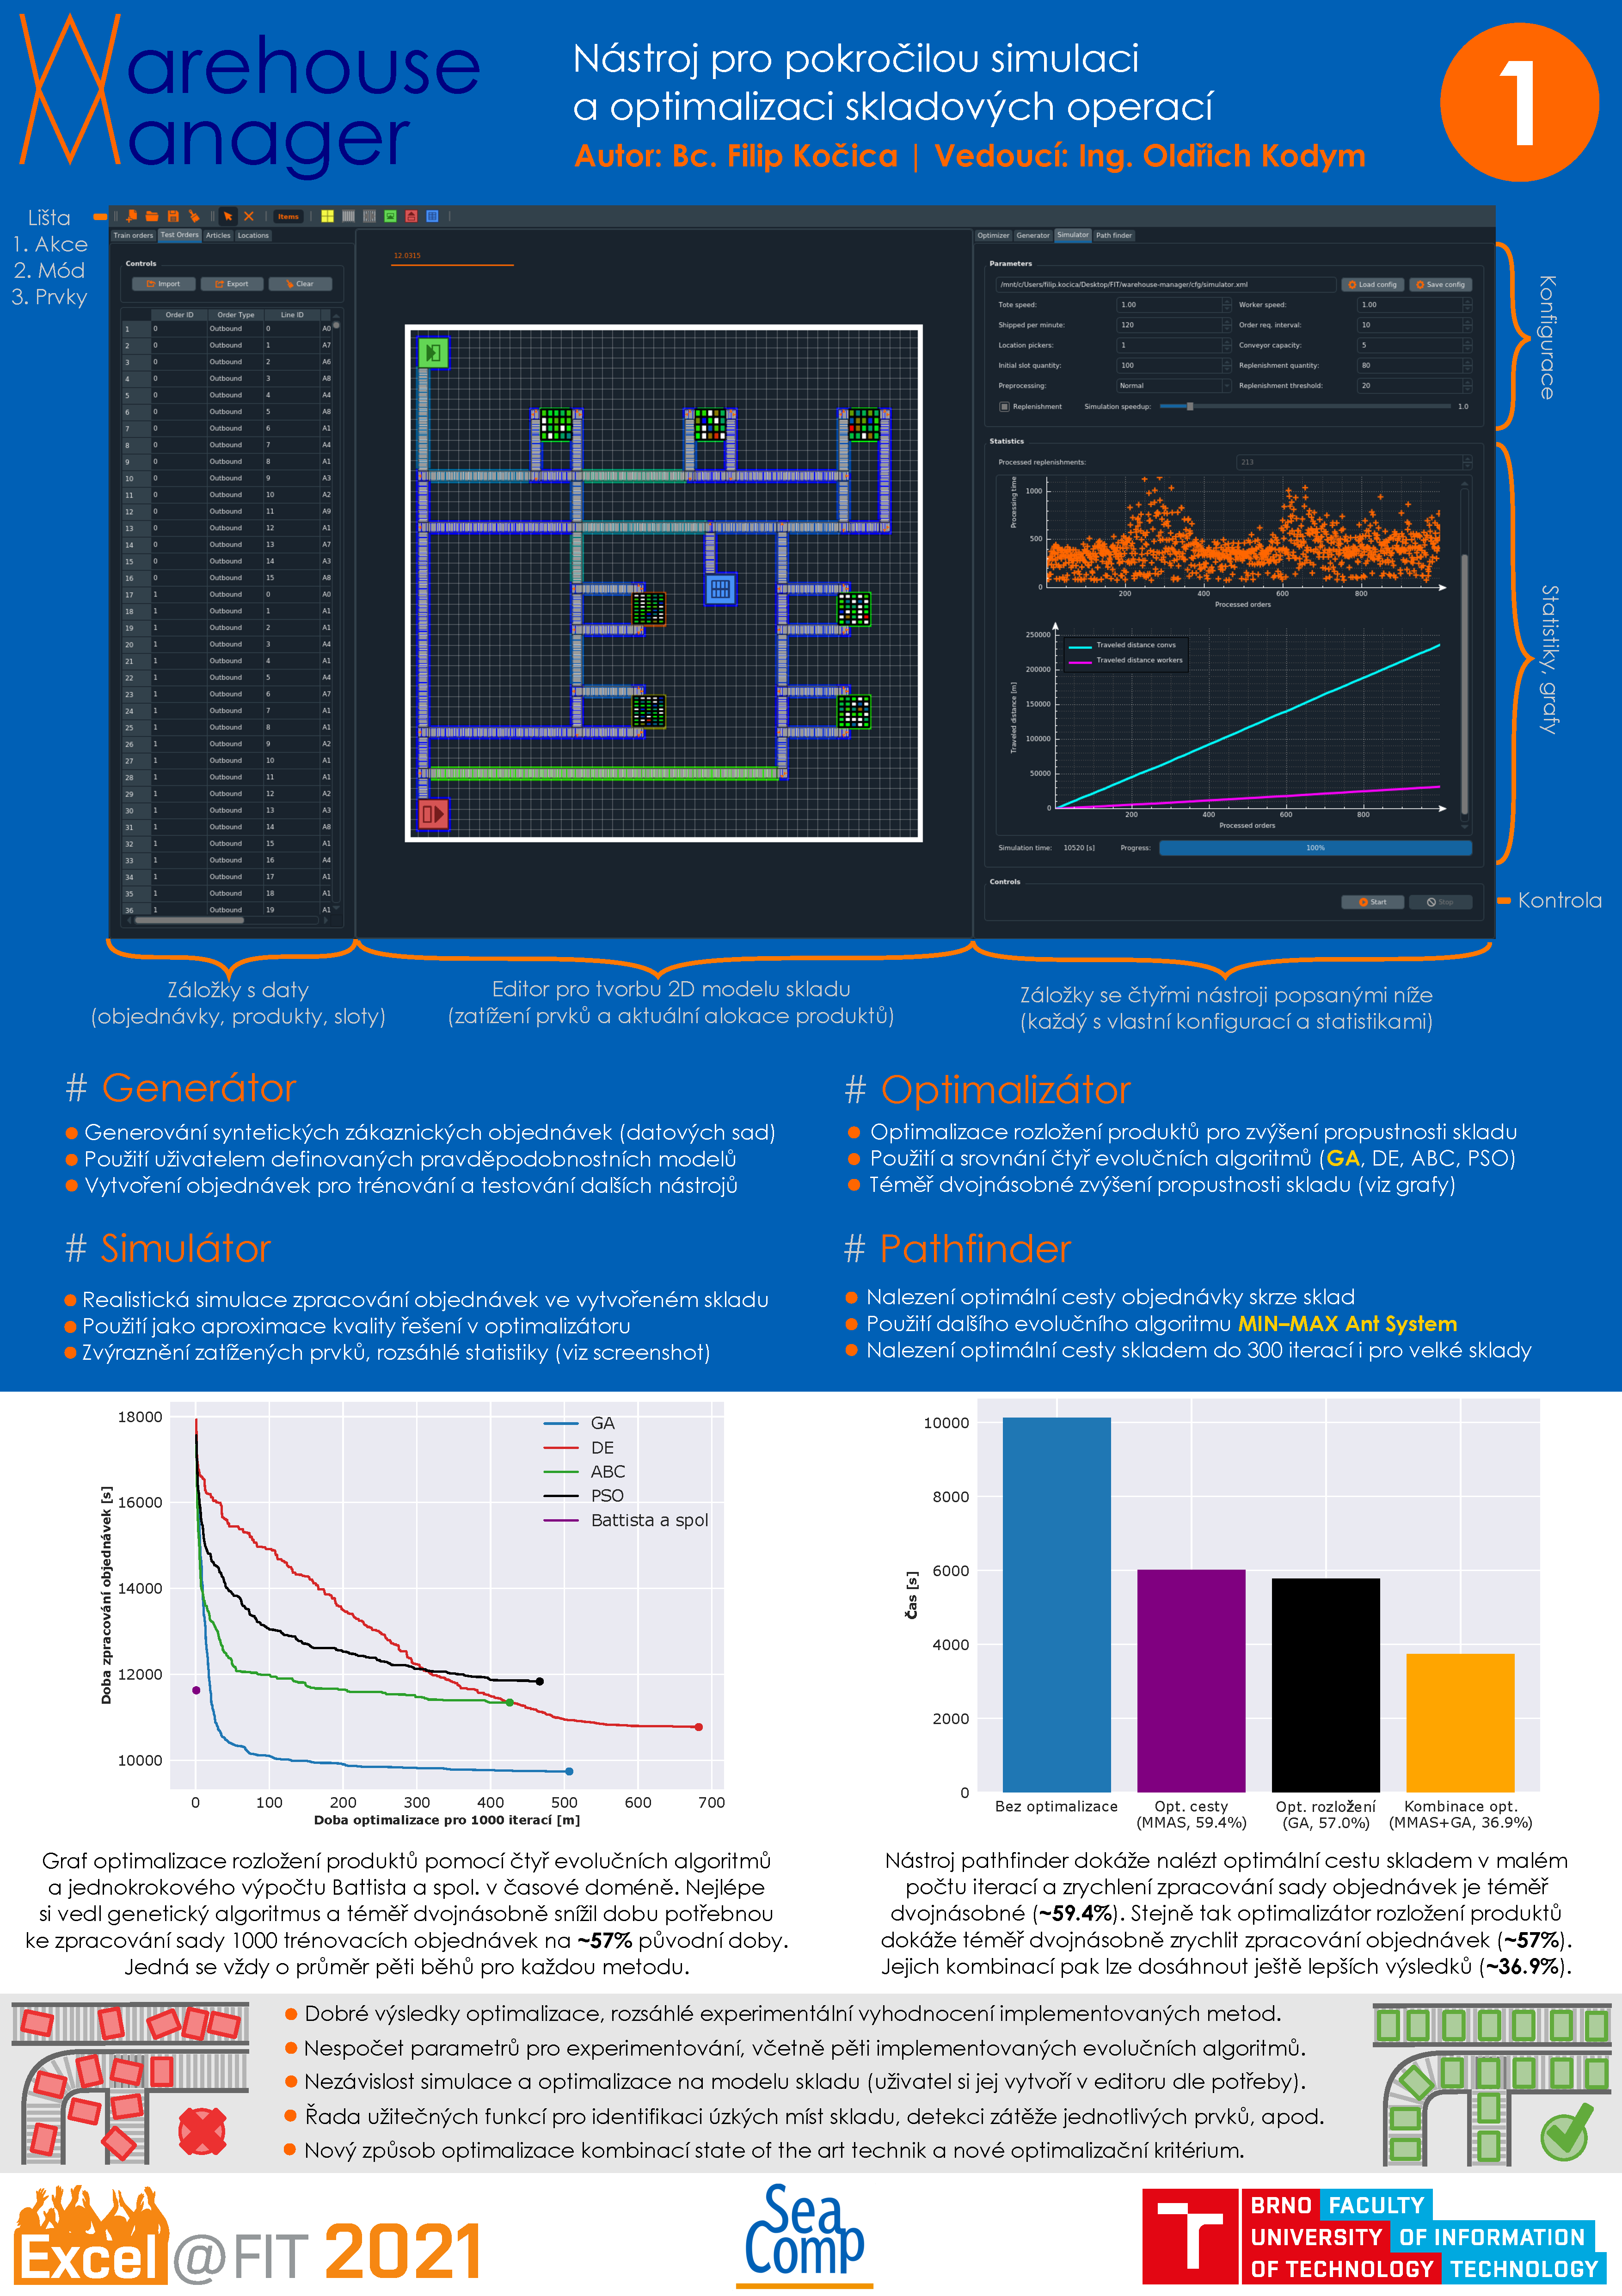
\includegraphics[width=0.75\linewidth]{figures/prilohy/poster.pdf}
\end{center}
  \fi
  
  % Kompilace po částech (viz výše, nutno odkomentovat)
  % Compilation piecewise (see above, it is necessary to uncomment it)
  %\subfile{projekt-30-prilohy-appendices}
  
\end{document}
